\documentclass[notombow,episode,openright,dvipdfmx]{kyouritu}
\usepackage{graphicx,color}
\usepackage{tikz}
\usepackage{makeidx,multicol}
\usepackage{amsmath,amssymb,amsthm}
\usepackage{standalone}
\usepackage{tocloft}
\usepackage{aliascnt}
\usepackage{ascmac}

% standard.sty から移動:
\usepackage{bm}
\usepackage[top=25truemm,bottom=20truemm,left=20truemm,right=20truemm]{geometry}
\usepackage{setspace} % setspaceパッケージのインクルード
\usepackage{wrapfig}
\usepackage{multicol}
\usepackage{ulem}
\usepackage{url}
\usepackage{array,arydshln}

\usepackage{hyperref}
\usepackage{pxjahyper}
%\usepackage{natbib} 
\usepackage{standard}

%プリアンブル
\topmargin -0.5in
\headheight 0.2in
\headsep 0.3in  
\evensidemargin -0.03in
\oddsidemargin -0.4in
%\textwidth 5.6in
%\textheight 8.4in
\renewcommand{\thetable}{%
\arabic{table}}

%圏点
\makeatletter
\def\kenten#1{%
\ifvmode\leavevmode\else\hskip\kanjiskip\fi
\setbox1=\hbox to \z@{・\hss}%
\ht1=.63zw
\@kenten#1\end}
\def\@kenten#1{%
\ifx#1\end \let\next=\relax \else
\raise.63zw\copy1\nobreak #1\hskip\kanjiskip\relax
\let\next=\@kenten
\fi\next}
\makeatother

%Section等先頭を大文字にすると番号付けしない.
\newcommand{\Chapter}[1]{\chapter*{{\Huge #1}}
\markboth{#1}{#1}
\addcontentsline{toc}{chapter}{#1}
\stepcounter{chapter}}
\newcommand{\Section}[1]{\section*{{\huge #1}}
\addcontentsline{toc}{section}{#1}}
\newcommand{\Subsection}[1]{\subsection*{\underline{#1}}}
\newcommand{\Subsubsection}[1]{\subsubsection*{#1}}
\setcounter{tocdepth}{0} %Chapterのみ表示する


\usetikzlibrary{%
  arrows.meta,%
  %decorations.pathreplacing,%
  decorations.markings,%
  shapes.misc,%
  patterns
}


\DeclareMathOperator{\supp}{supp}
\DeclareMathOperator{\inter}{int}

%Warizan
\def\hsymb#1{\mbox{\strut\rlap{\smash{\Huge$#1$}}\quad}}



%ito.tex
%これは他とぶつかったら変える予定です.

\newcommand\itomacro{
\newtheorem*{Thm}{定理}
\newtheorem*{Lemma}{補題}
\newtheorem*{Def}{定義}
\newtheorem*{Prop}{命題}
\newtheorem*{Ex}{例}
\newtheorem*{Prob}{問題}
\newtheorem*{Rem}{注意}
\def\qedsymbol{$\square$}
\def\proofname{\gt{証明}\;}
\newenvironment{Proof}{\par\noindent{\it\proofname}}{{\unskip\nobreak\hfill{\it\qedsymbol}}\par\vskip 9pt}
\newenvironment{Proof*}{\par\noindent}{{\unskip\nobreak\hfill{\it\qedsymbol}}\par\vskip 9pt}
\ifx\undefined\bysame \newcommand{\bysame}{\leavevmode\hbox to3em{\hrulefill}\,}\fi
\def\C{\mathbb C}
\def\N{\mathbb N}
\def\R{\mathbb R}
\def\Q{\mathbb Q}
\def\Z{\mathbb Z}
\newcommand{\Real}{\mathop{\mathrm{Re}}\nolimits}
\def\thm{\begin{Thm}}
\def\thmx{\end{Thm}}
\def\prop{\begin{Prop}}
\def\propx{\end{Prop}}
\def\defb{\begin{Def}}
\def\defe{\end{Def}}
\def\defx{\end{Def}}
\def\rem{\begin{Rem}}
\def\remx{\end{Rem}}
\def\prob{\begin{Prob}}
\def\probx{\end{Prob}}
\def\lem{\begin{Lemma}}
\def\lemx{\end{Lemma}}
\def\ex{\begin{Ex}}
\def\exx{\end{Ex}}
\def\cor{\begin{Cor}}
\def\corx{\end{Cor}}
\def\proof{\begin{Proof}}
\def\proofx{\end{Proof}}
\def\a{\alpha}
\newcommand{\Image}{\mathop{\mathrm{Im}}\nolimits}
\newcommand{\Ker}{\mathop{\mathrm{Ker}}\nolimits}
\newcommand{\Coker}{\mathop{\mathrm{Coker}}\nolimits}
\newcommand{\Aut}{\mathop{\mathrm{Aut}}\nolimits}
\newcommand{\Ho}{\mathop{\mathrm{H}}\nolimits}
\newcommand{\Res}{\mathop{\mathrm{Res}}\nolimits}

\def\TO{\Rightarrow}
\def\OT{\Leftarrow}
}

% arata.tex
\DeclareMathOperator{\RealPart}{Re}

% sato.tex
\newcommand\satomacro{
\def\vecb{\begin{pmatrix}}
\def\vece{\end{pmatrix}}
\def\detb{\left|\begin{matrix}}
\def\dete{\end{matrix}\right|}
\def\realnum{{\mathbb R}}
\def\dfrac{\displaystyle\frac}
\def\dsum{\displaystyle\sum}
\def\tenchi{{}^t\!}
\def\det{{\mathrm{det}}}
\def\rank{{\mathrm{rank}}}
\def\delxkf{\dfrac{\partial f}{\partial x_k}}
\def\delxp{\left(\dfrac{\partial}{\partial x}\right)_p}
\def\delyp{\left(\dfrac{\partial}{\partial y}\right)_p}
\def\delzp{\left(\dfrac{\partial}{\partial z}\right)_p}
\def\delxdp{\left(\dfrac{\partial}{\partial x'}\right)_p}
\def\delydp{\left(\dfrac{\partial}{\partial y'}\right)_p}
\def\delzdp{\left(\dfrac{\partial}{\partial z'}\right)_p}
\def\delxop{\left(\dfrac{\partial}{\partial x_1}\right)_p}
\def\delxkp{\left(\dfrac{\partial}{\partial x_k}\right)_p}
\def\delxnp{\left(\dfrac{\partial}{\partial x_n}\right)_p}
\def\delyofp{\left(\dfrac{\partial}{\partial y_1}\right)_{f(p)}}
\def\delykfp{\left(\dfrac{\partial}{\partial y_k}\right)_{f(p)}}
\def\delymfp{\left(\dfrac{\partial}{\partial y_m}\right)_{f(p)}}
\def\delxof{\dfrac{\partial f}{\partial x_1}}
\def\delxnf{\dfrac{\partial f}{\partial x_n}}
\def\delxkfo{\dfrac{\partial f_1}{\partial x_k}}
\def\delxkfm{\dfrac{\partial f_m}{\partial x_k}}
\def\delxofo{\dfrac{\partial f_1}{\partial x_1}}
\def\delxofm{\dfrac{\partial f_m}{\partial x_1}}
\def\delxnfo{\dfrac{\partial f_1}{\partial x_n}}
\def\delxnfm{\dfrac{\partial f_m}{\partial x_n}}
\def\xvec{(x_1,\dots,x_n)}
\def\avec{(a_1,\dots,a_n)}
\newtheorem{s_theo}{定理}
\newtheorem{s_defi}{定理}
\newtheorem{s_ex}{定理}

\def\qedsymbol{$\square$}
\def\proofname{\gt{証明}\;}
\newenvironment{Proof}{\par\noindent{\it\proofname}}{{\unskip\nobreak\hfill{\it\qedsymbol}}\par\vskip 9pt}
\newenvironment{Proof*}{\par\noindent}{{\unskip\nobreak\hfill{\it\qedsymbol}}\par\vskip 9pt}
\ifx\undefined\bysame \newcommand{\bysame}{\leavevmode\hbox to3em{\hrulefill}\,}\fi
}
%


%本文
\begin{document}
\frontmatter
\Chapter{まえがき}
\Chapter{まえがき}
前書きを書く前書き
(前書き著者より)
\clearpage % tocloft パッケージを使う場合は自分で \clearpage しないといけない
\tableofcontents
\mainmatter
%%まず最初に使ったプリアンブルをここに書いてください.
%ただしコンパイルの都合上コメントアウトしてください.
%実際に確認する際は,各自の環境でmain.texにこのプリアンブルを追加してください.

%\usepackage{mathrsfs}
%\usepackage[all]{xy}
%\newcommand{\proofend}{\begin{flushright} $\blacksquare$ \end{flushright}}
%\renewcommand{\labelenumi}{(\roman{enumi})}
%\newcommand{\nkgr}{・}
%\theoremstyle{definition}
%\newtheorem{theorem}{定理}
%\renewcommand{\thetheorem}{}
%\newtheorem{defi}{定義}
%\newtheorem{thm}[defi]{定理}
%\newtheorem{lem}[defi]{補題}
%\newtheorem{cor}[defi]{系}
%\newtheorem{prop}[defi]{命題}
%\newtheorem{ex}[defi]{例}


\Chapter{象の卵は美味しいぞう(伊藤)}
% タイトル(名前)でお願いします.
% セクションは \Section \Subsection \Subsubsection で分けてください.
% 詳しくはMAY2015を参考にしてください.
\Section{\S 0. はじめに}
本研究の真の目的は、一言で言えば、象の卵を見つけるという子供の頃からの夢をかなえることで
ある。
\Section{\S 1.研究目的}
本研究の目的は、象の卵の殻について、生物、化学、物理、工学などの方面から多角的に調べることである。象の卵の殻は、80kg を超える体重の子象と、その栄養源である卵黄の大きな質量を支えるだけではなく、卵を暖める親の象の体重も支える必要がある。このため、象の卵の殻は、体重の軽い鳥類 (図 1) の卵の殻とは本質的に異なる構造を持つ
\Section{\S 2.研究方法}
初年度は、まず世界の動物園を巡り、研究業績 [1] に可能性が示されたように象舍に卵が隠されて
いないか、探す。
2年目はアフリカに行き、空と地上から象の卵を探す。アフリカ象は気性が荒いが、サバンナの方
がジャングルよりも見通しが効くので、インドよりもアフリカを先に探索する。
3年目は、インドとタイに行き、ジャングルに隠されている卵を探す。ジャングルの場合は空から
は探しにくいが、象使いも多く、象の背中に乗って象の視点から探索することができる。さらに、気
だての優しいインド象ならば卵の在処を教えてくれる可能性もある。
ぞうの卵はおいしいぞう。ぞうの卵はおいしいぞう。ぞうの卵はおいしいぞう。ぞうの卵はおいし
いぞう。ぞうの卵はおいしいぞう。ぞうの卵はおいしいぞう。ぞうの卵はおいしいぞう。ぞうの卵は
おいしいぞう。ぞうの卵はおいしいぞう。ぞうの卵はおいしいぞう。ぞうの卵はおいしいぞう。ぞう
の卵はおいしいぞう。ぞうの卵はおいしいぞう。ぞうの卵はおいしいぞう。ぞうの卵はおいしいぞう。
ぞうの卵はおいしいぞう。ぞうの卵はおいしいぞう。ぞうの卵はおいしいぞう。ぞうの卵はおいしい
ぞう。ぞうの卵はおいしいぞう。ぞうの卵はおいしいぞう。ぞうの卵はおいしいぞう。ぞうの卵はおい
しいぞう。ぞうの卵はおいしいぞう。ぞうの卵はおいしいぞう。ぞうの卵はおいしいぞう。ぞうの卵
はおいしいぞう。ぞうの卵はおいしいぞう。ぞうの卵はおいしいぞう。ぞうの卵はおいしいぞう。ぞ
うの卵はおいしいぞう。ぞうの卵はおいしいぞう。ぞうの卵はおいしいぞう。ぞうの卵はおいしいぞ
う。ぞうの卵はおいしいぞう。ぞうの卵はおいしいぞう。ぞうの卵はおいしいぞう。ぞうの卵はおい
しいぞう。ぞうの卵はおいしいぞう。ぞうの卵はおいしいぞう。ぞうの卵はおいしいぞう。ぞうの卵
はおいしいぞう。ぞうの卵はおいしいぞう。ぞうの卵はおいしいぞう。ぞうの卵はおいしいぞう。ぞ
うの卵はおいしいぞう。ぞうの卵はおいしいぞう。ぞうの卵はおいしいぞう。ぞうの卵はおいしいぞ
う。ぞうの卵はおいしいぞう。ぞうの卵はおいしいぞう。ぞうの卵はおいしいぞう。ぞうの卵はおい
しいぞう。ぞうの卵はおいしいぞう。ぞうの卵はおいしいぞう。ぞうの卵はおいしいぞう。ぞうの卵
はおいしいぞう。ぞうの卵はおいしいぞう。ぞうの卵はおいしいぞう。ぞうの卵はおいしいぞう。ぞ
うの卵はおいしいぞう。ぞうの卵はおいしいぞう。ぞうの卵はおいしいぞう。ぞうの卵はおいしいぞ
う。ぞうの卵はおいしいぞう。ぞうの卵はおいしいぞう。ぞうの卵はおいしいぞう。ぞうの卵はおい
しいぞう。ぞうの卵はおいしいぞう。ぞうの卵はおいしいぞう。ぞうの卵はおいしいぞう。ぞうの卵
はおいしいぞう。ぞうの卵はおいしいぞ

{\itomacro%まず最初に使ったプリアンブルをここに書いてください.
%ただしコンパイルの都合上コメントアウトしてください.
%実際に確認する際は,各自の環境でmain.texにこのプリアンブルを追加してください.

%\usepackage{mathrsfs}
%\usepackage[all]{xy}
%\newcommand{\proofend}{\begin{flushright} $\blacksquare$ \end{flushright}}
%\renewcommand{\labelenumi}{(\roman{enumi})}
%\newcommand{\nkgr}{・}
%\theoremstyle{definition}
%\newtheorem{theorem}{定理}
%\renewcommand{\thetheorem}{}
%\newtheorem{defi}{定義}
%\newtheorem{thm}[defi]{定理}
%\newtheorem{lem}[defi]{補題}
%\newtheorem{cor}[defi]{系}
%\newtheorem{prop}[defi]{命題}
%\newtheorem{ex}[defi]{例}


\Chapter{代数学の基本定理でみる数学の世界(伊藤)}
% タイトル(名前)でお願いします.
% セクションは \Section \Subsection \Subsubsection で分けてください.
% 詳しくはMAY2015を参考にしてください.
\Section{はじめに}
数学科展示ますらぼにお越しいただきましてありがとうございます.
数学科とはどのようなことをやっている学科なのか一般の人に説明するのはなかなか難しく,
一般の人に端的な説明を求められるとなかなか四苦八苦してしまうところがあります.
この記事では数学科がどのようなことを勉強しているのかについて,
\textbf{代数学の基本定理}という定理を題材に出来るだけわかりやすく説明したいと思います.
この記事は第7回関西すうがく徒のつどいにおける拙講演「代数学の基本定理でみる数学の世界」を
更に詳しくして紙面化したものですので,講演に関してまとめたウェブ上の記事 http://togetter.com/li/878845 も参考にしていただければと思います.
\Section{代数学の基本定理とは}
代数学の基本定理とは
\thm
次数が$1$以上の複素係数一変数方程式には複素根が存在する
\thmx
という定理です.具体的にはどういうことを言っているのでしょうか.例を見てみましょう.
\ex
$2x-4=0$というのは$1$次方程式ですが$x=2$という解を持ちます.
\exx
\ex
$ax^2+bx+c=0$というのは$2$次方程式ですが,この方程式の解の公式も中学校で習ったことでしょう.
\exx
\ex
$3$次多項式と$4$次方程式にも,極めて難解ですが解の公式というものが知られています.
これについては"カルダーノの公式"や"フェラーリの公式"で調べてください.
\exx
これらの解の公式とは\underline{具体的にバッチリと解のありかを求める}公式です.
一方で代数学の基本定理とは複素根が存在すると言っているだけなので,\underline{どこにあるかは分からないけどとりあえず存在はするよ}という定理なんです.
しかし,これはどんな方程式にも解があるということを言っているのでそれは強い主張であるともいえます.
この定理は$1600$年ごろに様々な数学者によって予想され,$1800$年ごろにガウスによって証明がされました.
代数学の基本定理は高校生でも証明できるような定理なのですが,その基本的さ故に様々な証明があり,
大学$3,4$年生で習うようなことを使っても証明することができます.
この代数学の基本定理と共に大学の数学とはどのようなものなのかを見てみましょう.
\Section{大学1年生}
大学$1$年生で習う数学とは"解析学入門"と"線形代数学"の$2$つです.
どちらも数学の基礎であるとともに理系の多くの学科でも使われるものです.
\Subsection{解析学入門}
解析学入門は東大では"数学$1$"という科目名で開講されています.
微分と積分について現代数学的に学び直そうという科目です.
意識高く大学で勉強をしようと思っていた東大の$1$年生たちの多くがこの科目に打ちのめされて俗にいう五月病に羅患します.
この解析学のつまづきやすい$2$つのポイントとして,\large{$\epsilon-\delta$論法}と\large{コンパクト}というものがあります.
この$2$つについて見てみましょう.
\Subsubsection{$\epsilon - \delta$ 論法}
高校数学にも極限という概念はあって,$x$が$0$に限りなく近づくとか$n$が$\infty$に発散するとかいう言葉が使われています.これを厳密に定義しようというのが$\epsilon - \delta$ 論法です.
本格的な$\epsilon - \delta$ 論法に入る前に幾つか練習をしてみましょう.
\ex
ある$x$という実数の絶対値は全ての正の数$p>0$より小さいとします.これを数式で書くと以下のようになります.
\[
\forall p > 0 : \ |x| < p
\]
$\forall p$で全ての$p$についてということを言っているわけです.
ではこの$x$はどんな数なのでしょうか.$p=0.1$としてみても,$|x|$はこれより小さいです.$p=0.0001$としても$|x|$はこれより小さいです.
$p=0.000\cdots (0が2億個) \cdots 01$よりも$|x|$は小さいです.これはつまり$|x| = 0$ということです
$x$は$0$としたわけではないが,$0$になってしまった.これが現代数学の"限りなく近い"という概念をつかむのに大事な考え方です.
\exx
\ex
ある$x$という数は全ての正の数$p>0$よりも大きいとします.つまり,
\[
\forall p > 0 : \ x > p
\]
です.この$x$も具体的にはどんな数なのでしょうか.$p=1000$としてみても,$x$はこれより大きいです.$p=2億$としてみてもこれより大きいです.
これもやはり$x$は$\infty$であるということを示しているのではないでしょうか.$\infty$というのはきちんと定義されていませんが,
$x$は限りなく大きいとはこのような気分なんだなあということがイメージできます.
\exx
ではここで,$\epsilon-N$論法というのを見てみましょう.
\defb[$\epsilon - N$ 論法]
$\lim_{n\to\infty} a_n = \alpha $\\
$\iff$
$\forall \varepsilon > 0,\  \exists N \in \N \quad \textrm{s.t.}\  \forall n \in \N,\  n > N \Rightarrow |a_n - \alpha | < \varepsilon $
\defe
突然数式がたくさん出てきて混乱したかもしれませんが落ち着いて見れば簡単です.\\
$\lim_{n\to\infty} a_n = \alpha $というのを定義しているわけです.\\
$a_n$が$\alpha$に限りなく近づくとはどういうことをなのでしょうか.\\
それは,例で見たとおり,$|a_n - \alpha|$が限りなく小さくなればいいわけです.
それを表すために,$\varepsilon > 0$というとても小さな数を$1$つ取ってきます.
それに対して,ある$N$を取ってきて$N$以降では$|a_n - \alpha | < \varepsilon$が成り立っているよとするわけです.\\
例えば,$1000$項目以降では,$|a_n - \alpha| < 0.001$が,$100000$項以降では,$|a_n - \alpha | < 0.0000000001$が成り立っていたら
どんどん近づいて行くような気がしますよね.これが限りなく近づくよ,ということを言うためにまず$\forall \epsilon > 0$としているわけです.\\
\ex
$a_n = \frac{n+1}{n}$とすると$n \to \infty $でこれは$1$に収束します.\\
実際,$|a_n - \alpha| = | \frac{n+1}{n} - 1 | = | \frac{1}{n} |$です.\\
例えばこの$|a_n - \alpha|$を$0.01$より小さくしたい!と思えば,$N=100$としてあげれば,
$N$項目以降では$|\frac{1}{n}| < 0.01$が成り立つわけです.\\
ここでも,$|a_n - \alpha| $という差は$n$が大きくなるに連れてどんどん小さくなっていますね.
\exx
このような方法を採用するメリットとして,極限という概念がきっちりと定義されて,例えば,次のような明らかに成り立って欲しい極限の性質も厳密に証明する事ができます.
\prob
$\lim_{n\to\infty} a_n = \alpha , \lim_{n\to\infty} b_n = \beta $とする.\\
$\lim_{n\to\infty} (a_n + b_n) = \alpha + \beta , \lim_{n\to\infty} a_n b_n = \alpha\beta $
を示せ.
\probx
同様にして$\epsilon-\delta$論法も見てみましょう.
\defb[$\epsilon - \delta$ 論法による定義]
$\lim_{x \to a}f(x) = b$\\
$\iff$
$\forall \varepsilon > 0,\  \exists \delta > 0\quad \textrm{s.t.}\  \forall x \in \mathbb{R},\  0 < |x-a| < \delta \to |f(x)-b| < \varepsilon$
\defe
これも同様の考え方です.$x\to a\  (xがどんどんaに近づく)$のとき,$f(x) \to b\  (f(x)はどんどんbに近づく)$ということを定義しているわけです.また$|f(x)-b|$を限りなく小さくするために,$|x-a|$の幅を限りなく小さくとっているわけです.\\
またこの$\forall \exists$という並びは,どんな$\varepsilon (とても小さいイメージ)$に対してでも,いちいち$\delta (さらに小さいイメージ)$をとってくるということを表しています.
\prob
$\lim_{x\to 0} x^2 = 0$を証明せよ.$\varepsilon >0$として,$\delta = \sqrt{\varepsilon}$とすれば,$ 0 < | x | < \delta$ならば$ |x^2| < \varepsilon = \delta^2$を示せばよい. 
\probx
\Subsubsection{コンパクト}
次に第二のつまづきポイントであるコンパクトについて触れましょう.
高校数学で次のような定理があったことを思い出しましょう.
\thm[最大値最小値の定理]
$[a,b]$を有界閉区間,$f$を$[a,b]$上の実数値連続関数とする.
このとき$f$は最大値および最小値にそれぞれ少なくとも一点で到達する.
\thmx
これは高校数学では大した有り難みもない定理でしたが現代数学では重要です.
ここで重要なのは$[a,b]$が有界閉区間であるという仮定と,$f$は連続であるという仮定です.実際
\ex[非有界]
$\R$上で連続な関数$f(x)=x$は$\R$で最大値,最小値を持たない.
\exx
\ex[不連続]
$[-1,1]$上の関数.$f(x)=1/x$は最大値,最小値を持たない.
\exx
という例が示すように,有界閉区間または連続という仮定を外すとたちまちこの定理は成り立たなくなります.
この有界閉区間という概念を一般化したのがコンパクトです.
\defb[コンパクト]
$X$空間が$(点列)$コンパクトである\\
$\iff$
$X$内の任意の点列が$X$内に収束する部分列を含む
\defe
これも例を見てみましょう.
\ex
開区間$(0,1)$はコンパクトではない.なぜならば,$\{1/n\}$という数列は$0$に収束するが,この数列の部分列は$(0,1)$内の点に収束しない.
\exx
\ex
実数$\R$はコンパクトではない.なぜならば,$\{n\}$という数列は$\infty$に発散するが,この数列の部分列は$\R$内の点に収束しない.
\exx
\thm
$I \subset \R^n$がコンパクトであることと有界かつ閉であることは同値
\thmx
という風にコンパクトは有界閉区間の拡張になっているわけです.そして,
\thm
$I \subset \R^n$をコンパクト,$f$を$I$上の実数値連続関数とする.
このとき$f$は最大値および最小値にそれぞれ少なくとも一点で到達する.
\thmx
という定理が成り立ちます.こうして,$2$のポイントをおさらいしたところでその応用として代数学の基本定理を証明してみましょう.
\thm[代数学の基本定理]
次数が$1$以上の任意の複素係数一変数多項式$p(z)=a_0+a_1 z+\cdots + a_nz^n$には複素根が存在する.
\thmx
\proof[初等解析による証明]
これは杉浦光夫「解析入門1」に載っている証明です.
証明のポイントは3つ.\\
$(1)\ \lim_{|z|\to\infty}|p(z)| = \infty$\\
$(2)\ |p(z)|$はコンパクト集合上で最小値を取る.\\
$(3)\ |p(a)|>0 \Rightarrow \exists b \in \C \ s.t. \ |p(b)| < |p(a)|$(下には下がいる)
です.
\[
\lim_{|z|\to\infty}|p(z)| = \infty
\]
という意味をもう一度解釈してみましょう.
\[
\forall M \in \R \ \exists R>0 \ s.t. \  |z| > R \ \Rightarrow\  |p(z)|>M
\]
ということでした.そして$M$は任意ですから,$M=|p(0)|$として,それに対して$R>0$を一つ取り,
$K=\{ z\in\C |\ |z|\le R\}$とおけば,$K$の外では$|p(z)|>M$が成り立ちます.
つまりこの$K$の中で最小値を探せばいいいわけです.ところで$K$はコンパクトであるので
\begin{center}
$|p(z)|$は$K$上で最小値を取る
\end{center}
が言えます.最後に,
\[
|p(a)|>0 \Rightarrow \exists b \in \C \ s.t. \ |p(b)| < |p(a)|
\]
が言えて$(この証明は杉浦に譲ります)$証明終了.
\proofx
代数学の基本定理の証明は$1$年生の解析の大事な部分を使って得られるのでした.
\Section{大学2年生}
\Subsection{解析学続論}
大学$1$生では他に線形代数という科目を勉強しますが,この記事には関係ないので割愛します.
大学$2$年生では$1$年生で習った解析学と線形代数学の発展について学びます.
解析学では多変数の解析について学びます.ここでは線積分というものについて触れましょう.
今まで積分といえば,$\int_a^b$と言ったように区間$[a\ b]\subset \R$上での積分を考えてきましたが,
例えば,円周$\{(x,y)\in\R^2 | x^2+y^2=1\}$にそってある関数を積分したいということは数学だけでなく
多くの理系分野でよくあることです.まず曲線とは何かについて考えてみましょう.
\defb
$I\subset\R$を区間とします.$\phi:I \to \R^n$が空間曲線であるとは,一対一の連続写像であるこということである.
\defx
一対一というのは,$a\neq b \Rightarrow \phi(a) \neq \phi(b)$であるということで,つまりは自己交差をしないということです.
確かに自己交差をしなくてちゃんと繋がっていなくては曲線とはいえませんね.
\ex
$\phi:[0,1] \to \R^2$を$\phi(t)=(t,t)$で定める.これは$(0,0)$と$(1,1)$を結ぶ直線であり,空間曲線である.
\exx
\ex
$\phi:[0,2\pi) \to \R^2$を$\phi(t)=(\cos t ,\sin t)$で定める.これは単位円周です.
\exx
それではこれらの曲線にそった積分というのを次で定めます.
\defb
$f:\R^n \to \R$を関数,$\phi:I\to\R^n$を滑らかな曲線として,この曲線の像を$C$で表す.曲線$C$に沿った$f$の線積分を以下で定義する.,
\[
\int_C f(x)ds := \lim_{d(\Delta)\to 0} \sum_{i=1}^N f(\phi(\xi_i)) |\phi(t_i) - \phi(t_{i-1})|
\]
ただし,ここでの$\Delta$とは区間$I$の分割$t_0 < t_1 < \cdots < t_{N-1} < t_N$を考えており$d(\Delta)$はその分割の最も大きい幅です.
\defe
これはリーマン積分の考え方を使った積分の定義であり,詳しくは$e\pi isode\ vol.3$の"積分の歩み"を参照していただきたいのですが,
基本的には高校でならった区分求積法の考え方と同じで,区分求積法はある区間を同じ幅で分割していましたが,それを好きな幅で分割して良いようにしたという話です.またこの積分は収束して以下のようにも表されます.
\prop
$f,\phi,C$を上の定義と同様とし,$I=[a,b]$となるときに次が成り立つ.
\[
\int_C f(x) ds = \int_a^b f(\phi(x))|\phi'(t)|dt
\]
\propx
\ex
$f:\R^2\to\R$を$f(x)=1$という定数関数にして,$\phi:[0,1] \to \R^2$を$\phi(t)=(t,t)$で定める.\\
このとき
\[
\int_C f(x) ds = \int_0^1 |(1,1)| dt = \int_0^1 \sqrt{2}  dt  = \sqrt{2}
\]
です.この積分は$(0,0)$と$(1,1)$を結ぶ直線の長さ$\sqrt{2}$を求めています.
\exx
\Subsection{複素解析}
代数学の基本定理の証明方法に複素解析的な方法を使ったものが有名です.
複素解析は今まで実数関数でやってきたことを複素数の範囲に拡張することによって色々な美しい結果が得られる学問です.
複素解析の主な研究対象には正則関数というものがあります.まずそれを定義しましょう.
\defb[正則関数]
$f:\C \to \C$が正則であるとは各点で微分係数を持つということである.つまり,
\[
f'(z) = \lim_{h\to 0} \frac{f(z+h) - f(z)}{h}
\]
が各$z\in\C$で収束するということである.
\defx
\rem
これだけでは普通の実数の微分可能関数と変わらないではないかと思うかもしれませんが次のようことが成り立つことに注意しなければなりません.
つまり,$h\to 0$としていますがこの$h$は複素数なので色々な$0$への近づき方をするということです.
$h=x+yi$とおいて実部と虚部に分けたとき,$y=0,x\to 0$として$0$に近づけたときこれは偏微分$\frac{\partial f}{\partial x}$になります.
一方で$x=0,y\to 0$として$0$に近づけたとき,
\[
f'(z) = \lim_{y\to 0} \frac{f(z+yi)-f(z)}{yi} = -i\frac{\partial f}{\partial y}
\]
であり,
\[
f'(z) = \frac{\partial f}{\partial x} = -i\frac{\partial f}{\partial y}
\]
が成り立つ必要があります.この関係をコーシー・リーマンの関係式といいます.
\remx
次に$\C$の部分集合として重要な単連結領域というのを定義しますが,これは"便利な領域"として考えて頂いて構いません.
\defb[単連結領域]
$D \subset \C$が単連結領域であるとは,連結な開集合であって$D$内の任意の閉曲線は$1$点にホモトピックであるようなものである.
\defx
$1$点とホモトピックであるとはこの記事の後半を参照していただきたいのですが,単連結領域とは穴がない領域をイメージしてください.
そうすると以下のように重要な定理が成り立ちます.
\thm[コーシーの積分定理と積分公式]
$D$を単連結領域とし、$f(z)$ は $D$ 上で正則である複素関数とするとき、$C$ を $D$ 内にある長さを持つ単純閉曲線とする.
\[
 \oint_C f(z) \, dz\ = 0
\]
$a$をまた$C$によって囲まれる領域に属する点とする.
\[
 f(a) = \frac{1}{2 \pi i}\int_C \frac{f(z)}{z-a}dz
\]
\[
 f^{(n)}(a) = \frac{n!}{2 \pi i}\int_C \frac{f(z)}{(z-a)^{n+1}}dz
\]
\thmx
この定理の意味とは$f(z)$が正則であれば,どんな閉曲線上で積分してもその値は$0$になるということと,
逆に$a$という一点でだけ正則でないような$\frac{f(z)}{z-a}$という関数を積分するときは$f(a)$の値のみを考えればいいよという意味です.
この$e\pi isode$にある荒田さんの記事も参考になります.実際に例を見てみましょう.
\ex[コーシーの積分公式の例]
$f(z) = 1 , C = \{z\in\C | |z-a|=r\} $ のときコーシーの積分公式.\\
\[
1^{(n)}(a) = \frac{n!}{2 \pi i}\int_{|z-a|=r} \frac{1}{(z-a)^{n+1}} dz 
\]
となりますが
\[
 \int_{|z-a|=r} \frac{1}{(z-a)^{n+1}} dz =
  \begin{cases}
   \  2\pi i  \ \ (n=0) \\
   \  0 \ \ (n \ge 1) \\
  \end{cases}
\]
に他ならなりません.
\exx
正則関数がどれだけ関数に強い条件を課しているかというのは次の定理でわかります.
\thm[リュービルの定理]
複素平面全体で正則かつ有界な関数は定数関数のみ.
\thmx
\proof
\leavevmode\\
この証明は,藤本坦孝「複素解析」に載っている証明です.
証明のポイントは以下の$3$つです.\\
$(1)\ f有界つまり\forall z \in \C :\ |f(z)|\le M $かつ$f$正則を仮定する.\\
$(2)\  $仮定を満たす関数は正則より$f(z)=\sum_{n=0}^\infty c_n z^n $とべき級数展開可能\\
$(3)\ c_n$は$\forall R>0 : \ |c_n|\le \frac{M}{R^n}$をみたす.(ここでコーシーの積分公式が使われている)
\proofx
このリュービルの定理を用いて代数学の基本定理を証明する事ができます.
\proof[リュービルの定理を用いた代数学の基本定理の証明]
\leavevmode\\
この証明はLars Valerian Ahlfors「Complex Analysis」に載っている証明です.
証明のポイント:\\
$(1)\ p(z)=a_n z^n + \cdots + a_1 z+ a_0$が零点を持たないと仮定する(背理法)\\
$(2)\ g(z) = \frac{1}{p(z)}$は$\C$上で正則となる\\
$(3)\  \lim_{|z|\to\infty} |g(z)| = 0$となる.\\
$(4)\ $上から$g:$有界であることが言え,Liouvileより定数となり矛盾.
\proofx
複素解析の一つの目標として留数計算というものがあります.コーシーの積分公式では分数型の$1$点のみで正則でない関数の積分を考えましたが,
今度は他の形の正則でない点が複数ある場合でも積分計算をしてみようというというものです.
\defb[留数]
$f$が環状領域$\Delta(a,r,R) = \{z\in\C | \  r<|z-a|<R\}$で正則とする.このとき\\
\[
f(z) = \sum_{n=-\infty}^{\infty} a_n (z-a)^n
\]
という風に展開できて,これを$f$のローラン展開という.\\
特に$\Delta(a,0,R)$で正則$(a$のみ孤立して正則でない$)$とき,\\
$a_{-1}$のことを$f$の$a$での留数といい$\Res_{a} f$とかく.\\
\defx
\ex
$\frac{1}{z-c}$という関数を$|z|>|c|$でローラン展開すると.
\[
\frac{1}{z-c} = \frac{1}{z} + \frac{c}{z^2} + \frac{c^2}{z^3} + \cdots
\]
\exx
\thm[留数定理]
$D:$区分的$C^1$境界を持つ領域.$f:\overline{D}\setminus\{p_1,\cdots,p_n\}$で正則とする.
\[
\frac{1}{2 \pi i}\int_{\partial D} f(z)dz = \sum_{i=1}^n Res_{p_i} f
\]
\thmx
この留数定理とは,$f$という関数を積分する際は,$p_i$という点での留数のみを考えればいいよと言っているわけです.
留数を計算するのに便利な次の公式を紹介します.
\prop
$(1)\ z=a$に於いて$\lim_{z\to a} (z-a)f(z)$が有限確定値を持つとき,
\[
\Res_{a} f = \lim_{z\to a} (z-a)f(z)
\]
$(2)\ z=a$に於いて$\lim_{z\to a} (z-a)^m f(z)$が有限確定値を持つとき,
\[
\Res_{a} f = \frac{1}{(m-1)!} \lim_{z\to a} \frac{d^{m-1}}{dz^{m-1}} ((z-a)^mf(z))
\]
$(3)\ g,h$を正則関数として,$g(a)\neq 0,h(a)=0,h'(a)\neq 0$ならば
\[
\Res_{a} \frac{g}{h} = \frac{g(a)}{h'(a)}
\]
\propx
$\lim_{z\to a} (z-a)^m f(z)$が有限確定値を持つとき,$a$は$m$位の極であるといいますが,
$m$位の極の留数を計算するときは$(z-a)^m f(z)$という正則関数のテイラー展開を考えてあげればいいという話です.
正則関数の零点に関して次のような定理が成り立っています.
\thm[偏角の原理]
$D:$今までと同様.$f:$正則とする.
\[
\frac{1}{2 \pi i} \int_{\partial D} \frac{f'(z)}{f(z)}dz = (f\mbox{の}D\mbox{内の重複度込みの零点の個数})
\]
\thmx
\thm[ルーシェの定理]
$D:$区分的に$C^1$な境界を持つ有界領域\\
$f,g:D$とその境界上で定義された正則関数.\\
$\forall z \in \partial D :\ |f(z)-g(z)|<|f(z)|+|g(z)|$が成り立つとする.\\
このとき,$f$と$g$の零点の個数は等しい.
\thmx
ルーシェの定理は$f$と$g$の零点の個数を見たいときにその境界上のみで$f,g$の様子を考えて上げればいいという定理です.
\proof
\leavevmode\\
定理・証明ともに平地健吾先生に教えて頂きました.
証明のポイント\\
$(1)\ F_t(z) = (1-t) f(z) + t g(z)$は$0$にならない\\
$(2)\ N_t=\int_{\partial D} \frac{F_t'(z)}{F_t(z)}dz$は偏角の原理より$F_t$の零点の個数だがこれは$t$について連続.\\
$(3)\ (f$の零点の個数$)=N_0=N_1=(g$の零点の個数$)$
\proofx
%誰か良い例ください
この定理を用いて代数学の基本定理を証明する事ができます.
\proof[ルーシェの定理を用いた代数学の基本定理の証明]
\leavevmode\\

$f(z)=a_n z^n + \cdots + a_1 z+ a_0$と$g(z)=a_n z^n$とおく.\\
$|f(z)-g(z)|$は$n-1$次式,$|f(z)|+|g(z)|$は$n$次式より,\\
十分大きな円周上では$|f(z)-g(z)|<|f(z)|+|g(z)|$が成り立つ.\\
よって$f$の零点の個数は$n$個
\proofx
\prob
実はルーシェの定理まで行かなくても偏角の原理のみで代数学の基本定理を証明する事ができます.各自考えて見てください.
\probx
\Subsection{集合と位相}
ここでは位相空間論というものについて触れましょう.今までは$\R^n$のみで連続や収束という概念を考えて来ましたが,これを任意の集合に対して
扱えるようにするのが位相空間論の一つの目標です.

\defb[位相空間]
$X$を集合とする.$X$の部分集合からなる集合$\mathcal{O}$が$X$の開集合系である.\\
$\iff (1) (U_i)_{i\in I}$が $\mathcal{O}$の族ならば,$\cup_{i\in I} U_i \in \mathcal{O}$\\
$(2)(U_i)_{i\in I}$が $\mathcal{O}$の有限族ならば,$\cap_{i\in I} U_i \in \mathcal{O}$\\
また$\mathcal{O}$に属する元を$X$の開集合といい,$(X,\mathcal{O})$を位相空間という.
また閉集合とは開集合の補集合になっているものと定義します.
\defx
このようにして任意の集合に対して好きな開集合だけを集めてきて空間の構造を与えられることができるわけです.
\ex
自然数の集合$\N$に対して次のような位相を与えることができる.\\
$(1)$\ $\mathcal{O} = \{\emptyset , \N\}$\\
$(2)$\ $\mathcal{O} = \{U\subset\N | Uは\N の部分集合\}$\\
$(3)$\ $\mathcal{O} = \{ \N \setminus I | I\subset\N は有限部分集合\}$\\
これらの例は全て開集合系の定義を満たしていますので,これらにより$\N$を位相空間とできます.\\
$(1)$を密着位相,$(2)$離散位相.$(3)$を補有限位相と言います.
\exx
ここで収束を位相空間の言葉で書いてみましょう
\defb
位相空間$X$の点列$\{x_n\}$が$x$に収束する
\[
\iff\ \forall U :xを含む開集合 \ \exists N \in \N \ s.t.\ n \ge N \Rightarrow x_n \in U
\]
\defx
こう見てみると$U$とは$\varepsilon-\delta$のように$\varepsilon$とっていることがわかります.
つまり,位相空間とは開集合によって,集合に近いという考え方を与えているわけです.
こう考えてみると,$(1)$の密着位相は全ての点が同じ開集合に属しており,近いところにいるという意味で"密着"しています.\\
$(2)$の離散位相は,全ての$2$点は別々の開集合に入れることができるので"離散"しています.\\
ここで,集合に$(1)(3)$の場合の収束について見て見ましょう.
\ex
$x_n = n$という$\N$内の点列を考える.\\
このとき,$(1)(3)$の位相構造において$x_n$は任意の点に収束する.\\
$(1)$の場合.例えば,$1$に収束することを示してみましょう.$1$を含む開集合は$\N$だけですから,
$n \ge 1 \Rightarrow x_n \in \N$が成り立ちます.よって,$x_n$は$1$に収束します.\\
$(3)$の場合.$U$を$1$を含む開集合とします.これは$\{a_1,\cdots,a_n\}$という有限集合の補集合になっています.\\
よってこれらの最大値を$N$とおくと,$n \ge N+1 \Rightarrow  x_n \notin \{a_1,\cdots,a_n\}\ (最大値より大きいので)$が成り立つので,
\[
\iff\ \forall U :1を含む開集合 \ \exists N \in \N \ s.t.\ n \ge N \Rightarrow x_n \in U
\]
が示せました.同様にして,$x_n$は任意の点に収束することがわかります.一方で$(2)$の場合は$U=\{1\}$という開集合に対して$N$が取ってこれないので任意の点に収束しません.
\exx
次のような扱いやすい空間が定義されます.
\defb
$X:$位相空間,$A\subset X$ がコンパクトである.$\iff$
\[
A \subset \cup_{i\in I} U_i \Rightarrow \exists \{i_1,...,i_n\} \subset I s.t. \ A \subset U_{i_1} \cup \cdots \cup U_{i_n}
\]
\defx
\ex
$(1)(3)$はコンパクトである.$(2)$はコンパクトではない.
\exx

位相空間がコンパクトであるという概念については斎藤毅「はじまりはコンパクト」や斎藤毅「集合と位相」に詳しく解説されています.
また,最初に定義した点列コンパクトとコンパクトという概念は一致します.
\defb
$X$がハウスドルフ空間である.$\iff$\\
$x,y \in X , x\neq y \Rightarrow \exists U:x\mbox{の開近傍} ,\exists V:y\mbox{の開近傍} \ s.t. \ U \cap V = \emptyset$
\defx
\ex
$(1)(3)$はハウスドルフではない.$(2)$はハウスドルフである.
\exx
また連結という概念も位相空間の言葉を使って定式化することができます.
\defb
$X$が連結空間である.$\iff$\\
$X$の部分集合で開集合かつ閉集合であるようなものは,$\emptyset$と$X$のみ.
\defx
\ex
$(0,1) \cup (2,3)\subset\R$は連結空間ではない.\\
実際,区間$(0,1)$は開集合でかつ,$(2,3)$という開集合の補集合になっているので閉集合です.\\
これはこの区間が繋がっていないことによって起こる結果です.
\exx
ここで連続写像の概念も極めてシンプルに一般化されます
\defb
$f:X\to Y$が連続写像である.$\iff$\\
$U \subset Y$が開集合ならば$f^{-1}(U) \subset X$は開集合.
\defx
次の定理は,連続写像の性質を表すとともに,最大値最小値の定理と中間値の定理を一般化したものとも言えます.
\thm
$X,Y$を位相空間として,$f:X\to Y$を連続写像とする.\\
$(1)$$A\subset X$がコンパクトならば$f(A)\subset Y$もコンパクトである.\\
$(2)$$A\subset X$が連結ならば$f(A)\subset Y$も連結である.\\
\thmx
\rem
一方で\\
$(3)A\subset X$が開集合ならば$f(A)\subset Y$も開集合である.\\
$(4)A\subset X$が閉集合ならば$f(A)\subset Y$も閉集合である.\\
はどちらも一般には成り立ちません.これらが成り立つ写像をそれぞれ.開写像,閉写像といいます.
\remx
\proof[位相空間論における代数学の基本定理の証明]
この証明は斎藤毅「集合と位相」に載っている証明です.\\
$f:\C \to \C$を多項式が定める写像とすると,\\
正則関数の一般論から$f$は開写像であることが言える.\\
また$\C$の一点コンパクト化である$\C P^1$を考えることにより,$f$は閉写像であることがわかります.\\
よって,$\C$は連結空間で$f(\C)\subset\C$は開かつ閉であり,空集合でないので$f(\C)=\C$がいえます.\\
つまり,この多項式には$0$点が存在します.
\proofx
%ここまで書いた
\Section{大学3年生}
\Subsection{多様体}
多様体とは位相空間の中でも特に重要なもので,幾何学の主な研究対象です.
\defb[多様体]
$M:$が$n$次元の$(C^\infty 級)$多様体であるとは$M$がハウスドルフ空間であり,次のような開近傍$U_i$と同相写像$\phi_i : U_i \to \phi_i(U_i) \subset \R^n$が存在することである.\\
\[ \bigcup_i U_i = M \]
$U_i \cap U_j \neq \emptyset$のとき,次の座標変換がが$C^\infty$級である.
\[
\phi_i \circ \phi_j^{-1} | _{\phi_j(U_i\cap U_j)} :\phi_j(U_i\cap U_j) \to \phi_i(U_i\cap U_j)
\]
\defx
突然仰々しい定義が出てきましたが,多様体の$2$目の性質は局所ユークリッド的と言われるものです.
つまり,位相空間で連続写像については考えることが出来ましたが,微分を考えることはまだ出来ません.
そこで,位相空間のある一部を見てあげればそれはユークリッド空間であるとみなせるものを多様体としたのです.
つまり,多様体は好きなところに座標を入れることができ,かつ好きな用にいれた座標はちゃんとうまく合わさっているよというのがこの定義です.
幾何学の主な対称と言いましたが,例えば有名なポアンカレ予想は多様体に関する次のような定理です.
\thm[ポアンカレ予想]
\leavevmode\\
$M$多様体,$M$と$S^n$がホモトピー同値ならば$M$は$S^n$と同相である\\
$n=2$については$2$次元多様体の分類は$20$世紀はじめに知られており,
$n=3$コンパクトかつ単連結ならば$3$次元多様体は$S^3$と同相である.ということがポアンカレによって予想されました.\\
$n\ge 5$のときはスメールが解決,$n = 4$はフリードマンが解決,$n=3$のときはペレルマンが解決しました
\thmx
このように,数学の一つの目標にある概念を\underline{分類}するというものがあります.
分類することによって,今まで雑然と広がっていた世界が綺麗に掃除され見通しよくなるというのが数学の$1$つの仕事です.
では多様体での微分について定義しましょう.
\defb
多様体 $M_1, M_2$ を考える.写像 $F : M_1 \to M_2$ が $C^\infty$級であるとは、$F(x) \in M_2$ のまわりの座標近傍 $(V,\psi), F^{-1}(V)$ に含まれる$x\in M_1$ のまわりの座標近傍 $(U, \phi)$ に対して、
$\psi \circ F \circ \phi^{-1} : \phi(U) \to \psi(V )$が $C^\infty$ 級となることである。
\defx
ユークリッド空間内の多様体のみを考えて$f:M\to N$,$M\subset\R^k,N\subset\R^l$の微分を考える.\\
\[
df_x = (\frac{\partial f_i}{\partial x_j}):\R^k\to\R^l
\]
という行列で定める.\\
\defb
$x\in M$が正則点 $\iff df_x$が全射.\\
$x\in M$が特異点 $\iff df_x$が全射でない.\\
$y\in N$が正則値 $\iff f^{-1}(y)$が全て正則点.\\
$y\in N$が臨界値 $\iff f^{-1}(y)$が特異点を元として含む.\\
\defx

\proof[多様体論を用いた代数学の基本定理の証明]
\leavevmode\\
この証明はJohn Willard Milnor "Topology from the Differentiable Viewpoint"に載っている証明です.
証明のポイント\\
$(1)\ p(z):\C\to\C$を今までどおりの多項式とする.\\
$(2)\ h:S^2\to\C$というステレオグラフィック射影によって,\\
$(3)\ h^{-1}\circ p \circ h : S^2 \to S^2$を定める.\\
$(4)\ f$が$C^\infty$級写像であることを示す.\\
$(5)\ f$は有限個の臨界点しか持たない.\\
$(6)\ f$の球から正則値の集合は有限を除いたものなので連結.\\
$(7)\ \# f^{-1}(y)$は開近傍上で定数であるので常に0でない.\\
\proofx

\Subsection{群論}
代数学が扱う対称として基本的でシンプルなものが群です.群は集合に掛け算のみが入ったものを考えており,
例えば今まで習ってきた,整数や実数や群といったものは全て群です.群の定義は以下の様なものです.
\defb
集合$G$が群であるとは,$G$上の二項演算が$x,y,z\in G$に対して以下を満たすことである.\\
$\rm (i)$ $(xy)z=x(yz)$\\
$\rm (ii)$ $\exists e \in  G \ s.t. \ xe=ex=x$\\
$\rm (iii)$ $\forall x\in G \ \exists x^{-1} \in G \ s.t. \ x x^{-1} = x^{-1} x= e$\\
さらに,$xy=yx$を満たすとき$G$をアーベル群という.\\
\defe
また群の部分集合にも同じ演算の構造が入る場合に部分群といいます.つまり次のような定義です.
\defb
部分集合$H\subset G$が\\
$\forall x,y \in H: \ xy\in H$,\ \ $\forall x\in H:\ x^{-1} \in H$,\ \ $e\in H$\\
を満たすとき$H$を$G$の部分群という.
\defe
また部分群の中で扱いやすいものを定義します.
\defb
$N\subset G:$部分が正規部分群である\\
$\iff \ \forall g\in G : \ gNg^{-1} \subset N$
\defe
例えばアーベル群では全ての部分群は正規部分群です.
\defb
群$G$,$G'$があったとして,$f:G\to G' \  \forall x,y \in G \ f(xy)=f(x)f(y)$をみたす$f$を群準同型写像という.\\
特に$f$が準同型で全単射であるとき,同型写像であるという.
\defe
ここで群論で重要なシローの定理について触れておきましょう.
\defb
$G:$有限群,$p$:素数とする.$G$が$p$群$\iff\ |G|$が$p$のべき乗個.\\
$G$の部分群でかつ$p$群であるものを$p$部分群.\\
$|G|=p^e m, m,p$は互いに素なとき,\\
元の個数が$p^e$個の群をシロー$p$群という.
\defe

\thm[シローの定理]
$G:$有限群,$p$:素数とする.\\
$\rm (I)$シロー$p$部分群が存在する.\\
$\rm (II)$$(p\ $シロー部分群の個数$)\equiv\ 1 \bmod p$\\
$\rm (III)$$\forall P:シローp$群,$\forall Q:p$部分群,$\exists x\in G\  s.t. \ Q\subset xPx^{-1}$
\thmx
これは有限群を分類する際にとても便利な定理です.

\Subsection{ガロア理論}
ガロア論とは,体という四則演算が入った集合の拡大を考える理論で,体の拡大とそのガロア群を対応させることができるという理論です.
\defb
$K \subset L$に体の構造であるとき,$L$は$K$の拡大であるという.
\defx
\defb
$L$の同型で,かつ$K$上では恒等写像なもの全体を$\Aut_K(L)$とかく.
$\# \Aut_K(L)=[L:K]$のとき$L$は$K$のガロア拡大であるといい,$\Aut_K(L)$をガロア群という.
\defx
\ex
\[
[\C:\R]=2,\Aut_\R(\C) = \{\sigma_1,\sigma_2\}
\]
ただし,$\sigma_1$は恒等写像,$\sigma_2$は複素共役写像である.
\exx
\thm
$L/K$ を有限次ガロア拡大,$G$ をそのガロア群とする.
$(1)L/K$ の中間体 $M$ と $G$ の部分群 $H$の間に次の一対一対応がある:
\[
M \rightarrow G(L/M) , F(H) \leftarrow H
\]
$(2) M$ と $H $が対応するとき,$L/M$ はガロア拡大で $H$はそのガロア群である.
そして
\[
[L : M] = |H|, [M : K] = |G : H|
\]
$(3) M$ と $H$ が対応するとき,$M/K$がガロア拡大であることと$H$ が$G$ の正
規部分群であることは同値である.さらにこのとき
\[
G(M/K) \cong G/H. 
\]
\thmx
このガロア理論を用いても代数学の基本定理を証明する事ができます.
\proof[Galois理論による証明のポイント]
\leavevmode\\
雪江明彦「代数学2 環と体とガロア理論」に同様の証明が載っています.\\
$(1)\ K/\C$を有限次拡大とする.(背理法)\\
$(2)\ K/\R$は正規拡大であるとして一般性を失わない.\\
$(3)\ K/\R$はGalois拡大になる.\\
$(4)\ G:=Gal(K/R)$とする,$H\subset G$を2-Sylow群とすると,これに対応する拡大は奇数次拡大で,$\R$そのものしかない.\\
$(5)\ [K:\C]>1$で$2^n$であるとすると,$Gal(K/\C)$が2-群になって,$\C$が二次拡大をもつことになる.\\
\proofx
\Subsection{代数トポロジー}
多様体論では,
\defb
$X_n:$加群,$\partial_n:X_n\to X_{n-1}$の組が複体である.
$\iff\ \partial_{n-1} \circ \partial_{n} = 0$
\defe
\defb
ここで,$\Ker \partial_n =\{x\in X_n| \partial_n x = 0 \} $,\ $\Image \partial_{n+1} = \{ x_n \in X_n | \exists x_{n+1} \in X_{n+1} \ s.t. \ x_n = \partial_{n+1} x_{n+1}\}$\\
とおくと,$\Image \partial_{n+1} \subset \Ker \partial_{n}$は部分加群であり,$\Ho_n(X) = \Ker \partial_{n}/ \Image \partial_{n+1} $をホモロジー群という.
\defe
\defb
$\{X_n.\partial_n\},\{X_n'.\partial_n'\}:$複体とする.写像$f_n :X_n \to X_n'$が鎖準同型である.
$\iff\ f_{n-1}\circ\partial_n = \partial_n'\circ f_n$
\defe
\thm
$S^n=\{x\in\R^{n+1} | |x|=1\}$とすると,$\Ho_k S^n = \Z\  (k=0,n)$,$\Ho_k S^n = 0\  (k\neq 0,n)$
\thmx
\thm
$f:S^n \to S^n$を写像とすると,これは$f_*:\Ho_n(S^n)\to \Ho_n(S^n)$を引き起こす.\\
これは$\Z$間の準同型であるので,$f_*(x) = kx$とおけて,この$k$を$\deg(f)$と置いて,写像度という.
\thmx
\prop
$\rm (i)$$\deg(id)=1$\\
$\rm (ii)$$\deg(f\circ g) = \deg(f)*\deg(g)$\\
$\rm (iii)$$f \simeq g \Rightarrow \deg(f) = \deg(g)$\\
\propx


\proof[代数トポロジー的な代数学の基本定理の証明]
\leavevmode\\
この証明は,Albrecht Dold「Lectures on Algebraic Topology」に載っている証明です.
証明のポイント\\
$(1) \ \hat{p}:S^1\to S^1 ; z \to \frac{p(z)}{|p(z)|}$により定める.\\
$(2)\ |z|\le 1$ で 零点を持たないならば$\deg \hat{p} = 0$をしめす\\
$(3)\ p_t(z) =  \frac{p(tz)}{|p(tz)|}$による.\\
$(4)\ |z|\ge 1$ で 零点を持たないならば$\deg \hat{p} = n$.\\
$(5)\ p_t(z) =  \frac{t^kp(z/t)}{|t^kp(z/t)|}$による\\
\proofx
\Subsection{微分幾何学}
\defb
$\{g_p\}_{p\in M}$がRiemann計量である.\\
$\iff \ (1)g_p : T_p M \times T_p M \to \R $は内積.\\
$(2)s_1,s_2:U\to TM:$切断とすると,$g_p(s_1(p),s_2(p))$は$C^\infty$級・
\defe
\thm
$M$:境界つきコンパクトRiemann多様体. $K$を$M$のガウス曲率. $k_g:\partial M$の測地曲率.
\[
\int_M K\;dA+\int_{\partial M}k_g\;ds=2\pi\chi(M)
\]
\thmx
\proof[微分幾何学による代数学の基本定理の証明]
\leavevmode\\
この証明はhttp://arxiv.org/pdf/1106.0924.pdfに載っている証明です.
証明のポイント\\
$p(z)$が零点を持たないと仮定する.\\
$p^{*}(z) = z_np(1/z) = a_0z_n + a_1z{n-1} + \cdots + a_n$として, $f(z)=p(z)p^*(z)$とする.\\
$f(\tfrac{1}{w}) = p(\tfrac{1}{w})p^*(\tfrac{1}{w}) = w^{-2n}p^*(w)p(w) = w^{-2n}f(w)$\\
$w\in \C :\ g=\frac{1}{|f(w)|^{\frac{2}{n}}}\,|dw|^2$\\
$w\in \hat{\C} \setminus \{0\}:\  g=\frac{1}{|f(1/w)|^{\frac{2}{n}}}\,|d(1/w)|^2$ とする\\
$\frac{1}{|f(w)|^{\frac{1}{n}}}\,K_g=\frac{1}{n}\Delta \log|f(w)|=\frac{1}{n}\Delta \text{Re}(\log f(w))=0$
$\int_{\mathbf{S}^2}K_g=4\pi$により矛盾.
\proofx
\Subsection{確率論}
\proof[確率論による代数学の基本定理の証明]
この証明はL. C. G. Rogers , David Williams「Diffusions, Markov Processes, and Martingales: Volume 1, Foundations」に載っている証明です.
証明のポイントは.
$(1)\ (B_t:t \ge 0)$をブラウン運動とする.\\
$(2)\ f(z) = 1/p(z)$とおくと,これは正則で,$z\to\infty$で$0$に収束する.\\
$(3)\ \alpha < \beta$として$\{\Real f \le \alpha\}$と$\{\Real f \ge \beta\}$は開集合を含む.\\
$(4)\ f(B_t)$はマルチンゲールの収束から,$f(B_t)\to f(B_\infty)$に$L^1$収束する\\
$(5)\ $一方でこれはブラウン運動の再帰性に矛盾する.\\
\proofx
}
\Chapter{パズルのコーナー1.〜スリザーリンク〜(SP1)}
\Section{スリザーリンク}
\footnote{「スリザーリンク」「カックロ」の名称は(株)ニコリの登録商標です。}
\leavevmode \\
\\
\begin{figure}[h]
\centering
\includegraphics[width =7cm,bb = 0 0 202 202]{sp1slitherlink}
\end{figure}
\Subsection{スリザーリンクのルール}
\begin{description}
\item{1.} 点と点をタテヨコにつなげ、全体で1つの輪っかをつくります。
\item{2.}  4つの点で作られた小さな正方形の中の数字は、その正方形に引く辺の数です。数字のない小さな辺には、何本線を引くかは分かりません。
\item{3.} 線を交差させたり、枝分かれさせたりはしません。
\end{description}

%まず最初に使ったプリアンブルをここに書いてください.
%ただしコンパイルの都合上コメントアウトしてください.
%実際に確認する際は,各自の環境でmain.texにこのプリアンブルを追加してください.

%\usepackage{mathrsfs}
%\usepackage{amsmath}
%\usepackage[all]{xy}
%\newcommand{\proofend}{\begin{flushright} $\blacksquare$ \end{flushright}}
%\renewcommand{\labelenumi}{(\roman{enumi})}
%\newcommand{\nkgr}{・}
%\theoremstyle{definition}
%\newtheorem{theorem}{定理}
%\renewcommand{\thetheorem}{}
%\newtheorem{defi}{定義}
%\newtheorem{thm}[defi]{定理}
%\newtheorem{lem}[defi]{補題}
%\newtheorem{cor}[defi]{系}
%\newtheorem{prop}[defi]{命題}
%\newtheorem{ex}[defi]{例}


\Chapter{円周率$\pi$がひょこっと現れる話(山本)}
\Section{はじめに}

$e, \pi , i$の中で唯一義務教育までで習う数,それが円周率$\pi$です.
$3.14159 \cdots$という並びは皆さんも人生で一度は見たことがあるでしょう.
「円周率」の名の通り,$\pi$という数字は「円周の長さを直径で割ったもの」として定義される,図形由来の数です.円の面積を求めるときだったり,大学受験では回転体の体積を求めるときだったりに現れることが多いですね.
今日はこのように図形的な側面の強い円周率$\pi$が数学のひょんな所にひょこっと現れる話をしたいと思います.

(Caution:当文章においては,「大体どのような感じか」を理解していただくことを重要視するために,積分と無限和の順序を注意なしに交換する箇所が何か所かございます.あらかじめご了承ください.)

\Section{1.三角関数とFourier級数展開}

「$\pi$と関係する関数」と言われて,真っ先に思い浮かぶものは何でしょうか?
高校までの範囲でくくると,おそらく三角関数を連想する人が一番多いのではないでしょうか.
そこで,最初はこの三角関数についてお話しようと思います.

まず三角関数,特に$\sin \theta$や$\cos \theta$のグラフの形を思い出してみましょう.
これらのグラフは「正弦波」と呼ばれる綺麗な形の波になっています.
これは,音叉を叩いたときの音の波形などに現れます.
また,$\sin \theta$や$cos \theta$は
\[
\sin ( \theta +2 \pi )= \sin \theta, \cos( \theta +2 \pi )= \cos \theta
\]
なる関係を満たしていました.
これは $\theta$ がちょうど$2 \pi$増えたときの関数の値が元のものと同じであること,すなわち$2 \pi$が関数の周期になっていることを意味します.
より一般に,関数$f(x)$に対して$f(x+2 \pi )=f(x)$が成り立つとき,$f(x)$は$2 \pi$を周期として持つといいます.
これに沿えば,正の整数$n$に対して,$\sin (n \theta ), \cos (n \theta)$もまた$2 \pi$を周期として持つことが分かります.

このように,$2 \pi$を周期に持つ関数の簡単な例として三角関数が挙げられます.
これらは比較的簡単な形をしており,解析もしやすいです.
さて実際には周期$2 \pi$の関数はこれだけではないわけで,音や振動を解析する際には単純な正弦波の形をしていないものを対象とする場合がほとんどです.
そのような場合の関数はどのように扱うのがいいでしょうか?

大学1年で習うTaylor展開は,関数をある点の付近で多項式により近似するものでした.
これに倣うと,「一般の関数をより簡単な関数の和で近似する」ことを考えるのがいいかもしれません.

18〜19世紀の数学者Fourierは,「すべての周期関数は,同じ周期を持つ無限個の三角関数の和で表される」という主張をしました.
この主張は元々熱伝導に関する問題を解く際に用られたものであり,主張を認めればその問題の解にたどり着くことができたのでした.Fourierによるこの大胆な主張は,真偽が定かでなかったために数学界に議論を巻き起こしましたが,結果的には「大体」正しい主張であったことが後に分かります.
主張がどこまで正しいのか・また正しいとして,その無限和の収束やふるまいは良いものか?という当時の問いは,その後の解析学,ひいては数学そのものを大きく発展させたと言われています.

さて,Fourier級数展開の具体的な主張を見てみましょう.
\begin{center}
$f(x)$を「性質の良い」周期$2 \pi$の関数とする.
このとき,
\begin{equation}
	f(x)=a_{0}+\sum_{n=1}^{\infty}\left( a_{n}\cos(nx)+b_{n}\sin (nx) \right)
	\label{f1}
\end{equation}
となるような実数$a_n, b_n$($n$は自然数)が存在する.
\end{center}
ここで,「性質の良い」というのは,例えば「定義域全体で微分可能で,さらに導関数も連続」などが相当します.
上に出てきた各係数$a_n, b_n$は,大雑把には次のように計算されます.
まず$a_0$については,(\f1)の両辺を$x$について$0$から$2 \pi$まで積分して
\begin{eqnarray*}
	\int_{0}^{2 \pi}f(x)dx &=& \int_{0}^{2\pi} \left( a_{0}+\sum_{n=1}^{\infty}\left( a_{n}\cos(nx)+b_{n}\sin (nx) \right) \right) dx \\
	&=& \int_{0}^{2 \pi} a_{0} dx +\sum_{n=1}^{\infty} \int_{0}^{2\pi}\left( a_{n}\cos(nx)+b_{n}\sin (nx) \right) \right) dx \\
	&=& 2\pi a_{0}+0=2 \pi a_{0}
\end{eqnarray*}
すなわち
\[
	a_0=\frac{1}{2\pi}\int_{0}^{2 \pi}f(x)dx
\]
を得ます.正の整数$m$に対する$a_m$については,次の公式
\begin{eqnarray*}
	\int_{0}^{2 \pi} \cos (nx) \cos (mx) &=&
	\begin{cases}
		\pi & (n=m) \\
		0 & (n \neq m) \\
	\end{cases}
	\\
	\int_[0}^{2 \pi} \cos (nx) \sin (mx) &=& 0
\end{eqnarray*}
を使えば,次のように計算できます.
(\f1)の両辺に$\cos mx$をかけ,それを$x$について$0$から$2 \pi$まで積分すると
\begin{eqnarray*}
	\int_{0}^{2 \pi} \cos (mx) f(x) dx &=& \int_{0}^{2 \pi} \cos (mx)\left( a_{0}+\sum_{n=1}^{\infty}\left( a_{n}\cos(nx)+b_{n}\sin (nx) \right) \right) dx \\
	&=& \int_{0}^{2 \pi} a_{0} \cos (mx) dx +\sum_{n=1}^{\infty} \int_{0}^{2\pi} \cos (mx)\left( a_{n}\cos(nx)+b_{n}\sin (nx) \right) \right) dx \\
	&=& \pi a_{m}
\end{eqnarray*}
を得ます.すなわち,$m \ge 1$に対して
\[
	a_{m}=\frac{1}{\pi} \int_{0}^{2 \pi} \cos (mx) f(x) dx
\]
となります.同様にして,$b_m$も
\[
	b_{m}=\frac{1}{\pi} \int_{0}^{2 \pi} \sin (mx) f(x) dx
\]
と計算できることになります.これで,係数が計算できました.

それでは,とある関数を実際に三角関数の無限和で表してみましょう.

周期$2 \pi$の関数$f(x)$を,$0 \le x \le 2\pi$において$f(x)=-x(x-2 \pi)$となるように定めます.
これは$x=2\pi n$($n$は整数)において微分可能ではありませんが,先に述べた「性質の良い」関数の1つです.
これを認めれば,積分計算により$a_0, a_n, b_n$を求めてやることで$f(x)$を三角関数に表すことが出来ます.
実際に計算してみると(部分積分を使えば高校生にもできる計算ですので,やってみてください),
\begin{eqnarray*}
	a_0 &=& \frac{2}{3}\pi ^2 \\
	a_n &=& -\frac{4}{n^2} \\
	b_n &=& 0
\end{eqnarray*}
となるので,結局
\[
	f(x)=\frac{2}{3}\pi ^2-\sum_{n=1}^{\infty} \frac{4}{n^2} \cos (mx)
\]
と表すことができました.

さて,上式に$x=0$を代入してみましょう.
すると
\[
	0=\frac{2}{3}\pi ^2-\sum_{n=1}^{\infty} \frac{4}{n^2}
\]
となり,適当に整理すると
\[
	\sum_{n=1}^{\infty} \frac{1}{n^2} = \frac{\pi ^2}{6}
\]
となりました.
これはすなわち,「自然数の二乗の逆数の和が$\pi ^2 /6$になる」ということを意味しています.
左辺は整数に関する基本的な級数になっているわけですが,その値として$\pi$がひょこっと現れるという不思議な公式が出来てしまいました.
この級数は「Basel級数」と呼ばれています.

他にも,Fourier級数展開を使うと導ける級数は色々あります.
関数を色々変えてみて,様々な公式を作ってみるのも興味深いかと思います.

\Section{$\zeta$ 関数,$\Gamma$関数と関数等式}

前章において,自然数の二乗の逆数の和の値に$\pi$が現れることを見ました.
では,「二乗」が「$n$乗」,あるいは実数「$s$乗」と変わった場合の値はどうなるのでしょうか?

そこで,$1$より大きい実数$s$に対して,$\zeta (s)$(ゼータ)という関数を
\[
	\zeta (s) = \sum_{n=1}^{\infty} \frac{1}{n^{s}}
\]
により定義します.
ここで「$1$より大きい実数」と言ったのは,$1$以下の実数では定義式の級数が発散してしまうことを考慮してのことです.
この$\zeta$関数の定義式から,前章のBasel級数は$\zeta (2)$に相当します.
実は,正の偶数$n$に対して,$\zeta (n)$は$\pi ^{n}$と有理数の積の形をしていることが知られています.

「正の偶数」という規則正しい数値を代入すると$\pi$に関係する値を返す$\zeta$関数ですが,この関数まわりで$\pi$が出てくるのは,関数に何かしらの値を代入するときだけではありません.

それを説明するために,$zeta(s)$とは別の関数として,$s>0$なる実数に対して$\Gamma (s)$(ガンマ)という関数を
\[
	\Gamma (s) = \int_{0}^{\infty} e^{-t}t^{s-1}dt
\]
により定義します.
$cdots$いきなり積分の式が出てきてしまいましたが,これがどのような関数なのか説明します.
部分積分を行えば,$s>0$なる実数$s$に対して
\begin{eqnarray*}
	\Gamma(s+1) &=& \int_{0}^{\infty} e^{-t}t^{s}dt \\
	&=& \left[ -e^{-t}t^{s} \right]_{t=0}^{\infty} - \int_{0}^{\infty} (-e^{-t})(st^{s-1})dt \\
	&=& 0+s\int_{0}^{\infty} e^{-t}t^{s}dt =s\Gamma(s)
\end{eqnarray*}
となることが分かります.
この$\Gamma(s+1)=s\Gamma(s)$のように,ある種の関数が満たしている等式のことを「関数等式」といいます.
また,とくに
\[
\Gamma(1)=\int_{0}^{\infty} e^{-t}dt=1
\]
となるので,上の関数等式と合わせれば,数学的帰納法により全ての正の整数$n$に対して
\[
	\Gamma(n)=(n-1)!
\]
となることが分かります.
つまり,$\Gamma$関数とは「正の整数でしか定義されなかった階乗の定義域を拡張したもの」ということになります.
ある意味で整数論由来の関数というわけですね.

さて,$\Gamma$関数は階乗の定義域を拡張したものと述べました.
しかし,この関数は更に「ほとんどの複素数」にまで定義域を拡張することができます.
高校までの数学では,関数といえば定義域は実数のものがほとんどだったかと思いますが,大学での数学では定義域を複素数にすることもしばしばあります.

例えば,$y=x^2$という関数は定義域を複素数としても「自然に」定義できますし,$y=1/x$という関数は定義域を「$0$以外の複素数」としてもやはり「自然に」定義できます.
指数関数$e^x$についても,$e^x$をTaylor展開して
\[
	e^x = \sum_{n=0}^{\infty} \frac{1}{n!}x^{n}
\]
という関数として考えれば,やはり複素数全体に定義域を「自然に」拡張することができるでしょう.
これらと同様にして,$\Gamma$関数も「自然な方法により」,定義域を「ほとんどの複素数」とする関数にすることができます.
具体的には,「複素数全体のうち,$0$以下の整数を除いたもの」全体を定義域とすることができます.

$\Gamma$関数についての話が長くなりましたが,ようやく$\zeta$関数の話に戻ります.
$\Gamma$関数同様,$\zeta$関数も「自然な方法で」定義域を拡張することができます.
さらに,この$\zeta$関数の現れる関数等式を得ることもできます.
ここまで出てきた関数を組み合わせて
\[
\Lambda (s)=\pi ^{-s/2} \Gamma(\frac{s}{2}) \zeta (s)
\]
という関数を定めます.
(ただし,複素数$s$に関して,$\pi ^s = e^{s \log \pi }$と定めると,これは定義域が実数の場合の拡張になっています.)
このとき,この関数について
\[
\Lambda (s)=\Lambda(1-s)
\]
という関数等式を得ることができます.
この等式はすなわち,「$\Lambda (s)$は点$s=1/2$に関して対称な関数であること」を意味する,かなり簡潔かつ綺麗な式になっていることが分かるかと思います.
$Gamma$関数,$\zeta$関数といういわば「整数論由来の」関数における簡素な関数等式を導くという方向からも,$\pi$が現れてくるわけです.
ちなみに,先ほど定義域を広げることが出来るといった$\zeta$関数ですが,関数等式を用いることにより,負の偶数$n$に対して$\zeta (s)=0$となることが分かります.
それ以外で$\zeta (s)=0$となるような複素数$s$はどのような分布の仕方をしているか?という問いは「Riemann予想」と呼ばれ,最初に提唱されてから150年以上経った今でも未解決です.

\Section{3.Ramanujanと$\pi$}
先の章で,無限和による$\pi$の公式(Basel級数)を1つ見ました.
他にはどのような公式があるのでしょう?そこで,突然ながらこの公式をご覧ください.
\[
\frac{1}{\pi}=\frac{\sqrt{8}}{99^2} \sum_{n=0}^{infty}frac{(4n)! (1103+26390n)}{(4^{n}n!)^{4}99^{4n}}
\]
$cdots$なかなかに面妖な格好をしています.
この公式を見出したのは「インドの魔術師」という異名を持つ,Ramanujanという数学者です.Ramanujan本人はこの公式を証明したわけでなく,実際に証明されたのは提唱されてから50年以上経ったころのことだそうです.
にもかかわらず,このようにかなり複雑な公式をRamanujanはいきなり発見したのですから驚きです.
これ以外にも,Ramanujanは$\pi$に関していくつかの公式を発見しています.

また,Ramanujanは$\pi$に関する公式以外にも様々なことをやっています.
例えば,次の関数をご覧ください.
\[
	\Delta (q)=q(1-q)^{24}(1-q^{2})^{24} \cdots = q\prod_{n=1}^{\infty}(1-q^n)^24
\]
これはRamanujanの$\Delta$(デルタ)関数と呼ばれるものです.
$\Delta$関数を$q$に関して「展開」すると,
\[
	\Delta (q)=q-24q^{2}+252q^{3}-1472q^{4}+\cdots
\]
のようになります.
これは$q$に関する多項式のようなもの(正式にはべき級数といいます)になっているわけですが,これの$q^n$における係数を$\tau (n)$とおきます.
すなわち:
\[
	Delta (q)=q\prod_{n=1}^{\infty}(1-q^n)^24 = \sum_{n=1}^{\infty} \tau (n) q^{n}
\]
です.
この関数$\tau$を「Ramanujanの$\tau$(タウ)関数」といいます.
また,$\Delta(q)$の定義式の$q$として$q=e^{2\pi iz}$を代入することができ,そうすると
\[
	F(z)=\sum_{n=1}^{\infty} \tau (n) q^{n}=\sum_{n=1}^{\infty} \tau (n) e^{2 \pi inz}
\]
は虚部が正である複素数全体を定義域とする関数となります.
$\Delta$および今作った$F$は,次の性質を満たします.
(3つ目の性質を証明することは若干難しいです.)
\begin{itemize}
	\item $\Delta (q)$は$q$に関するべき級数
	\item $F(z+1)=F(z)$
	\item $F(-1/z)=z^12 F(z)$
\end{itemize}
この性質により,$F$および$\Delta$は「重さ$12$の保形型式」であるといいます.
さらに,
\begin{itemize}
	\item $\Delta(0)=0$
\end{itemize}
が成り立つことにより,$F$および$\Delta$は「重さ$12$のカスプ型式」であるといいます.
保形型式・カスプ型式は整数論的にも歴史のある関数です.
さて,実際に$\tau (n)$を計算してみると,こんな感じになります.
(計算力に自信のある人は試してみてください.)
\begin{eqnarray*}
\tau(1)=1, \tau(2)=-24, \tau(3)=252, \tau(4)=-1472 \\
\tau (5)=4830, \tau(6)=-6048, \tau(7)=-16744, \tau(8)=84480 \\
\tau(9)=-113643, \tau(10)=-115920, \tau(11)=534612, \tau(12)=-370944
\end{eqnarray*}
これらの数字を見て何か気付くことはあるでしょうか?
もし即答できたら,あなたもRamanujanになれるかもしれない!?

実際のところ,Ramanujanはおおよそ次のようなことに気付きました:
\begin{itemize}
	\item 互いに素な整数$n,m$に対し$\tau(n)\tau(m)=\tau(nm)$
	\item 素数$p$,正の整数$n$に対し$\tau(p^{n+1})=\tau(p) \tau(p^{n})-p^{11}\tau(p^{n-1})$
\end{itemize}
$n,m$を小さめの数字にして確認してみると,
\begin{eqnarray*}
	\tau(4)=-1472=(-24)^2-2^{11} \cdot 1=\tau(2)\tau(2)-2^{11}\tau(1) \\
	\tau(6)=-6048=-24 \cdot 252 = \tau(2) \tau(3)
\end{eqnarray*}
となり,なるほど確かにそうなっているように思えます.
そしてこの考察は的中していたことが後に証明されました.
Ramanujanの洞察力の凄まじさを思い知らされます.

さて,前章でRiemann予想について少しだけ触れましたが,$\zeta$関数を考察する一つの方法として,$\zeta$関数を単体で見るのではなく,何らかの関数のクラスの$1$つであると見てやるというものがあります.
そのような「関数のクラス」として,保形型式から得られる「保形$L$関数」というものがあります.
今回は,$\Delta$関数から保形$L$関数を作り,その中でやはりひょっこり$\pi$が登場することを見たいと思います.

といっても定義自体は簡単で,保形$L$関数$L_{\Delta}(s)$は
\[
	L_{\Delta}(s)=\sum_{n=1}^{\infty}\frac {\tau (n)}{n^s}
\]
により,実部が十分大きい複素数$s$で定義することができます.$zeta$関数の定義式を少し変えただけですね.
そうなるとやはり,$zeta$関数と似た性質を持つことが期待されます.

ここで突然ですが
\[
\Lambda (s)=\int_{0}^{\infty}F(iy)y^{s-1}dy
\]
という値を考えてみます.
$F(iy)$が$y \rightarrow \infty$で「非常に速く」$0$に収束すること,および先に挙げた$\F$の性質から$F(i/y)=y^12F(iy)$となることを使えば,$\Lambda(s)$は全ての複素数$s$で値を持つことが分かります.
また,
\[
	F(iy)=\sum_{n=1}^{\infty}\tau(n) e^{-2\pi yn}
\]
だったことを思い出せば,$\Lambda(s)$は次のように計算できます:
\begin{eqnarray*}
	\Lambda (s) & = & \int_{0}^{\infty}F(iy)y^(s-1)dy \\
	& = & \int_{0}^{\infty}\left(\sum_{n=1}^{\infty}\tau(n) e^{-2\pi yn} \right) y^{s-1}dy \\
	& = & \sum_{n=1}^{\infty}\tau(n) \int_{0}^{\infty}e^{-2\pi yn}y^{s-1}dy
\end{eqnarray*}
ここで
\[
	\int_{0}^{\infty}e^{-2 \pi yn}y^{s-1}dy
\]
において,変数変換$t=2 \pi ny$により,
\begin{eqnarray*}
	\int_{0}^{\infty}e^{-2 \pi yn}y^{s-1}dy & = & (2 \pi n)^{-s}\int_{0}^{\infty}e^t t^{s-1}dy \\
	$=$ (2\pi)^(-s) \times \Gamma(s) \times n^(-s)
\end{eqnarray*}
となります.よって,
\begin{eqnarray*}
	\Lambda (s) $=$ \sum_{n=1}^{\infty}\tau(n)(2 \pi)^{-s}\Gamma(s)n^{-s} \\
	&=& (2 \pi )^{-s}\Gamma(s)L_{\Delta}(s)
\end{eqnarray*}
となっていることが分かります.
よく分からない積分の式から$L_{\Delta}(s)$が現れ,また再び$\pi$がひょこっと出てきました.
$Lambda(s)$が全ての複素数に対して定義できていたことから,
\[
	L_{\Delta}(s)=(2 \pi)^s \Lambda(s)/ \Gamma(s)
\]
により$L_{\Delta}(s)$の定義域を複素数全体に拡張することができます.
これが,$\Lambda(s)$なるものを考えた理由の1つです.
$Lambda(s)$を考えた理由はもう1つあります.
$Lambda(s)$の定義式にある$y$について,$t=1/y$と積分変換すると,
\begin{eqnarray*}
	\Lambda(s) &=& -\int_{\infty}^{0}F(i/t)t^{-(s-1)}frac{dt}{t^2} \\
	&=& \int_{0}^{\infty}t^{12}F(it)t^{-(s+1)}dt \\
	&=& int_{0}^{\infty}F(it)t^{(12-s)-1}dt
	&=& \Lambda(12-s)
\end{eqnarray*}
となることが分かります.
これにより,$L_{\Delta}$に関する関数等式
\[
	(2 \pi)^{-s}\Gamma(s)L_{\Delta}(s)=(2 \pi)^{12-s}\Gamma(12-s)L_{\Delta}(12-s)
\]
が導かれました.
$\zeta$関数のとき同様,底を$\pi$の何乗かとする指数関数を掛け合わせることによって,かなり綺麗な形の関数等式を得ることができました.

\Section{おわりに}
今回は$\pi$が「ひょこっと」現れる話ということで,図形的な概念でないところから$\pi$が出現するというものをいくつか挙げてみました.
(後半はかなり解析的整数論の話になってしまいましたが(汗))
今回挙げたもの以外でも$\pi$が現れるところは色々ありますし,また$\pi$でなくても,全く関係がないと思われていた分野に別概念がいきなり現れるということはしばしばあります.
皆さんも,興味があればそういったものを探してみてはいかがでしょうか?

\Chapter{パズルのコーナー2 〜算数パズル〜(SP1)}
\Section{算数パズル1.虫食い覆面算}

\begin{figure}[h]
\centering
\includegraphics[width =7cm]{sp1puzzle1}
\end{figure}

ま,す,ら,ぼの4文字には互いに異なる数字が入ります。

\Section{算数パズル2.等式作り}
四角のますをちょうど2つ消して,正しい式を作りましょう。
\begin{figure}[h]
\centering
\includegraphics[width =12cm]{sp1puzzle2}
\end{figure}

\Chapter{第一回 数学科意識調査!}
数学科の人ってなに考えてるかわからない。数学のことしか考えてないの?そんなことを、よく言われてしまいます。\\
そこで、今回は数学科のB3・B4、計18人にアンケートをとり、数学科に通う学生の生態を探りました。読み物程度に眺めてみてください。

\Section{数学をやりたいと思ったのは?}
まずは、数学をやりたいと思ったきっかけをインタビュー。18人中、8人が「中学のころ」、5人が「高校のころ」と答え、全体の3/4を占めました。やはり、『数学』という科目の出会いが、運命を大きく変えたのでしょう。\\
{\bf 数学オリンピックとか部活(数学研究会)でのゼミとか(ペンネーム:simplicial object)}や、{\bf ポアンカレ予想のドキュメンタリーを見て(普遍性)}など、学生時代からすすんだ数学の一端に触れていた人が、ここ数学科には多く集まっています。\\
中には、「小学校以前」から数学を志していた人も!{\bf 小学生の時にあたしンちに「因数分解」という単語が出てきて,調べてみたら面白かった.小6にやたらと塾の先生が「この問題は微積を使うと解ける」というので,インターネットで調べてみると面白かった.(後藤夢乃)}ということでまずは数学が好きになり、さらに{\bf 高校生のときに物理の先生と一緒に群論・環論の本をよんでいて面白かった.(後藤夢乃)}ということで現代数学にハマっていったと、熱く語ってくれました。\\
しかし、東大の特徴として「2年生の冬に学部・学科といった進路を決める」というものがあるので、当然大学生になってから数学に目覚めた人もいます。中には{\bf 昔から数学が好きだった事と、医学部での勉強に嫌気がさして(zatamura)}ということで、別の大学からこの東大理学部数学科に移ってきた人も!降年(希望の学科に行くため、1年留年すること)して、数学科を目指す人も少なくありません。そんな熱意を持った人があつまっているのです。

\Section{数学をやっててよかったことは?}
「サインコサインや、ビブンセキブンなんて、いつ使うの?」数学はしばしば「生きてて役に立たない」と思われがちです。そこで数学科の学生に、数学ができて(数学をやってて)よかったと思うことを聞いてみました。\\
{\bf 自分の頭の中をいかに人に伝えるかをとても考えるようになりました。(花屋のワルガキ)}というのが、とても印象的な回答でした。難しいことを難しく伝えるよりも、難しいものを噛み砕いて伝える方が何倍もエネルギーを使います。数学科でゼミなんかをやってると、こういったことはしょっちゅう鍛えられるのです。{\bf 論理的に物事を考えられるようになったこと(いぬい)}という回答もありましたが、このような力はたとえば就活でも活きてきます。\\
しかし大部分を占めるのは、{\bf 綺麗な証明や定理に出会って感動できる(GAP)}や、{\bf 単純に生涯ハマれるような趣味ができたこと。(ごま)}、{\bf 数学に関して真剣に議論できる友達が出来た}といった、数学の世界にどっぷりハマっているからこそ得られる喜びです。{話題が尽きたら適当な数学概念を説明することで会話が弾む(マスク)}、{\bf 等しいことと同型なこと違う概念だと気がつき、またそれに敏感になれた(こばけん)}というのは、既に学部生ながら研究者の風格があります。中には{\bf 特に無し(zetamura)}と断言してくれた人も。数学の世界には、数学を志す者にしかわからないよろこびが待っているのです。\\
最後に、{\bf 研究室に時間的に拘束されない}とか{\bf 多少面倒な説明書も楽々読めます}といったライフスタイルに関わるものもあったと報告しておきます。中でも、これは羨ましいと思う人も多いのでは…?\\
{\bf 中高生の頃は、数学を教えてほしいと女の子に囲まれた。その内の1人が今の彼女です$>\_<$(髭)}

\Section{数学以外のことを考えているときは?}
数学以外のことを考えているときは、どんなことを考えていますか?いくつかの選択肢を付けて聞いてみました。(複数選択可)
{\bf 眠い(12人)}というのが最多でした。大学生の性ですね。数学科の午前中の授業開始時刻は9時15分と、他の学科よりもやや遅いものの、それでも眠いものは眠いんです!仕方ない!\\
{\bf お腹すいた(10人)}{\bf お酒が欲しい(7人)}{\bf 彼女欲しい(7人)}が後に続いて、三大欲求に正直だなあと思いました。{\bf バイト行かなきゃ(6人)}{\bf サークル行かなきゃ(4人)}という風に他に打ち込んでるものがある人も。バイトだと知り合いには塾・家庭教師だけでなく、喫茶店で働いてる人もいます。サークルは音楽系(特にオーケストラ)が多い印象です。\\
{\bf アニメ観たい(5人)}は期待を裏切らないですね。学部生のフリースペース、学部生室には、アニメの原作になっている漫画(けいおん、キルミーベイベーや、聲の形まで)が揃っています。また。数学以外の勉強を楽しんでたり、{\bf だいたいプログラミング(Ziphil)}という人もいます。さらに自由回答欄では筋肉をつけたい人が2人ほどいました。数学の問題も、筋肉ですべてを解決したいものです。

\Section{数学の魅力って?}
数学科の意識調査なのだから、せっかくなので数学の話もしましょう。専門にしたいことと、その魅力を語ってもらいました。
{\bf 視覚数理科学、応用なので役に立つ(淘汰)}という意見がありますが、これは筆者の私の専門も関わるところです。応用数理に近いような解析系は、数学科の中でも魅力を語りやすいと言われています。{\bf 色々な分野(解析学・確率論・応用数理など)の知識を活かすことができる.色々な分野(経済・物理等)に活かすことができる.}と答えてくれた人がいますが、数学科の有力な就職先の一つに経済分野があります。「数学ならだれにも負けない」という学生が、求められているのです。\\
解析を離れたところでは、{\bf ホモトピー論、素朴なのに数学の言語って感じだ(simplicial object)}{\bf 代数幾何 代数の人とも幾何の人とも話ができて楽しいです(たつろー)}と答えてくれました。中でも、数論(整数まわりの研究)をやろうとしている人は熱く語ってくれています。{\bf 数論 数の美しさを感じる(zetamura)}{\bf 保形関数論:いい感じの関数が数論的情報を持ってくるのが神秘的(ばんほーてん)}といった風に。整数論は「数学の女王」と言われる分野ですが、熱意を持った研究者たちが女王に謁見すべく力を注いでいます。\\
数学の根幹を探ろうとする人も。{\bf 集合論; ZFCを越えた先に広がる世界を見ることができる(GAP)}詳しくは『公理的集合論』『ラッセルのパラドックス』で調べてもらうのがよいのですが、我々が数学を扱うときに基本となる『集合』。これが何かを表す公理系が『ZFC』(ツェルメロ=フレンケルの公理系に選択公理を加えたもの)だと言われています(現在これが使われているというだけで、もしかしたら覆されるかもしれない…)。ここで語るのはあまりに難しいので、ぜひ「ますらぼ」のブースにいる人に聞いてみてください。

\Section{さいごに・おまけ}
ここまで読んでいただきありがとうございました。数学科の人はこんなこと考えてるんだよ、こわくないんだよ、ということがお伝えできてればいいなと思います。
最後に、「無人島にひとつだけ何か持っていけるとしたら、どんな数学書を持っていきますか? 」という質問をしてみました。こんなふざけた質問に真面目に答えてくれる数学科のみんながとてもすきです。\\
幾何からは{\bf categorical homotopy theory},{\bf 位相幾何学},{\bf 離散幾何学講義}。解析・応用系からは{\bf complex analysis}{\bf ルディンのReal and complex analysis}{\bf Lambda Calculus with Types}。集合論だと{\bf Kunenの集合論},{\bf Handbook of Set Theory (Volume 3)}。代数幾何が人気で、{\bf ハーツホーンの代数幾何学},{\bf EGA(代数幾何原論)}がかなり票を集めていました。\\
もちろんちゃんと無人島に行くことを考えて、{\bf 食べられる数学書},{\bf EGA(燃料と食料として良さそう)},{\bf EGA…野生動物を殴る},{\bf 解析系。解析系の式を砂浜に書き殴りたいですね。}というロマンある回答が見られました。最後の一人の回答は{\bf 持って行かない}…そりゃあそうだな。
\Chapter{数学科で勉強すること(仮)(大澤)}
\Section{代数}
\Subsection{はじめに}
中学高校では代数というと、「数字だったものが文字に変わり、それらの計算を考える」という意味にとられることが多いでしょう。\\
$2 + 3 = 5$だったものが$2a + 3a = 5a$に置き換わる。人によってはとりとめのない変化だと感じる人もいるでしょう。
数学科の代数ではどのようなことが起きるかというと、「数字の一般化」だけでなく、「集合の一般化」「演算の一般化」が行われていきます。\\
数字が文字に変わったとはいえ、中学高校の頃はそいつらの正体は所詮"実数"の中のお話だったし、"足し算"や"掛け算"というのもよく知っているものでした。これらを一般化していくとどうなっちゃうの?といったお話を、これからしていこうと思います。\\
(ちなみに、"実数"ってなんだろう、"自然数"って「1とか2みたいなやつら」じゃ定義にならないよね、ということを考えるのも立派な数学ですよ!!)

\Subsection{群とは}
群(ぐん)というのは、演算が入った集合に、最低限のルールを加えたものです。\\
最低限のルールさえあれば、別に集合の中身は実数じゃなくてもいいし、演算も足し算や掛け算じゃなくても構いません。変な話、「ペンとアッポーでアッポーペン、ペンとパイナッポーでパイナッポーペン」みたいな計算規則でもよいのです。\\
必要最低限の規則とは、「計算が集合の中で完結してること」、「結合法則が成り立っていること」、それから大事なのが「単位元と逆元の存在」です。例えば掛け算なら、どんな数でも1という数を掛け合わせれば結果は変わらないですよね。このように計算結果を変えないものを『単位元』といいます。また、0以外の数には逆数と呼ばれるものがあって、$3 × 1/3 = 1$という風に計算結果を1にすることができますよね。これが『逆元』です。このとき、「0を除く実数は掛け算に関して群をなす」といいます。\\
掛け算じゃ面白くないので、別の例を考えます。「瀧くん、三葉ちゃん、奥寺先輩」の3人がいるとします。瀧君と三葉ちゃんが入れ替わることを$(瀧、三葉)$と書くことにします。さらに瀧君が入った三葉ちゃんと奥寺先輩が入れ替われば、瀧君に三葉ちゃんが、三葉ちゃんに奥寺先輩が、奥寺先輩に瀧君が入ることになります。この3人が順繰り入れ替わっている状況を、$(瀧、三葉)$と$(三葉、奥寺先輩)$の掛け算だと考えます。この入れ替わりの計算は、群をなします。「入れ替わらないこと」が単位元であり、また例えば$(瀧、三葉)$を2回やれば元に戻るので逆元もあります。この群を『対称群』といいます。\\
人数が増えても任意の入れ替わりは、このように二人の入れ替わりを繰り返せば実現できます。これが「あみだくじ」の原理です。あみだくじがどんな入れ替わりも再現してくれるのは、この対称群のおかげなのです\\
ということで、いろんな集合、いろんな演算を無限に思いつくことができるのですが、たとえば「瀧くん、三葉ちゃん、奥寺先輩の入れ替わり」と「オバマ、クリントン、トランプ3人の入れ替わり」は、集合の元は違いますが実質的に同じですよね。もっと詳しく言うと、2つの群の間に演算を保つような1対1対応(写像)があるとき、2つの群は実質的に同じものであり、『群同型』であるといいます。群同型なものをまとめて扱うとき、たとえば元の数が100個の群は何種類あるか考える、という問題が思い浮かぶでしょう。

\Subsection{環・体とは}
群で多少はっちゃけすぎたので、環・体は真面目にやります。\\
環・体には2つの演算が登場します。それぞれ、「足し算のような役割」と「掛け算のような役割」を果たします。これらにそれぞれ最低限の規則を与えて(例えば"足し算"の方は群の性質に加えて交換法則も必要だが、"掛け算"の方は逆元が必要ない)、分配法則が成り立つようにしたものを環(かん)といいます。さらに、"掛け算"にも交換法則が成り立ち、"割り算"もできるようにしたものを体(たい)といいます。\\
環になってくると、より"数字"に近いものを扱うようになります。整数や、$a + b\sqrt{2}$といった形の集合は環。有理数、実数、複素数のようなものは体になります。\\


体の"割り算"は完全に割り切ることになるのですが、環で"割り算"を扱うときは"商""余り"を考えることになります。\\
高校数学で、整式の割り算を扱ったと思います。あれも"商""余り"を考える整数のような扱い方をしましたが、じゃあ正式にも"素数"のようなものはあるのか。また、さっき挙げた$a + b\sqrt{2}$という集合は"素因数分解"できるのか。こういった概念を一般化するのが環の醍醐味です。\\
数字や多項式といったイメージしやすいものから、解析の世界に現れる作用素環というものまで、環の種類は様々です。群ほど自由度はありませんが、あらゆる場面に現れます。

\Subsection{体の上の線形空間}
といっても、群や環はかなり抽象的な数学で、数学が得意な学生であっても初めは戸惑う人の方が多いです。これらは数学科では、3年生の授業で扱います。\\
抽象数学の入り口として、理系の1,2年生は線形空間というものを扱います。高校数学でおなじみ『ベクトル』を扱うことになるのですが、$ベクトル = 矢印$というイメージからは離れてもらうことになります。ここでは、以下のような性質を満たせばベクトルということになります。

\[
Kを体とするとき、VがK上のベクトル空間であるとは、任意のKの元a,bと任意のVの元u,v,wに対して
\]
\[
(u + v) + w = u + (v + w)
\]
\[
u + v = v + u
\]
\[
ある0 \in V が存在して任意のvに対して v + 0 = v
\]
\[
任意のv \in V に対して (-v) \in Vが存在して v + (-v) = 0
\]
\[
a(u + v) = au + av
\]
\[
(a + b)v = av + bv
\]
\[
a(bv) = (ab)v
\]
\[
1 \in K(Kの単位元)としたとき 1v = v
\]
をみたすことである。



これは矢印だけでなく、例えば$ax^2 + bx + c$といった多項式も、a,b,cを体の元とすればベクトルになります。\\
例えば空間のベクトルであれば、線形独立な3つの矢印を使ってすべての矢印を表現できますが、さっきのような多項式の話でも例えば$x ^ 2$,$x$,1に適当な数字をかけて足し合わせることですべての二次以下の多項式を表現できます。つまり、二次以下の多項式をすべて集めた集合は、ベクトル空間であるということができるのです。\\
引き続き多項式のベクトル空間を考えます。$x^2$を微分すると$2x$,$x$を微分すると1になりますが、これは二次以下の多項式の空間を一次以下の空間に移すことになります。このようにベクトル空間同士の写像を考えることになるのですが、これは行列を使って表されます(今の高校生は習わないようですが)。行列は数を2行2列、3行3列…などと並べたものなのですが、写像の性質を調べたいときに行列を使って話を進めることになります。行列の基本的な扱い方は1年生で学習します。\\
このようにベクトル空間を扱う学習を「線形代数」というのですが、数学科に内定が決まった2年生の後半まで続きます。そのころになってくると、ベクトル空間の間の写像を集めて、新しい空間として考える『双対空間』、2つのベクトル空間の"積"のようなものを考える『テンソル積』といったように、理解に時間がかかるような題材を扱うことになります。線形代数は大学数学の入り口だと言われることが多いですが、数学科でやる線形代数はかなり手ごわく、そのぶん極めれば抽象数学の魅力がたっぷり詰まっていると言えるでしょう。
\Section{幾何}
\Subsection{はじめに}
幾何というと図形問題。高校数学まではその一言で片づけられる気がします。\\
初等幾何学の中にも実は様々な種類があるのですが、おそらく馴染みがあるのはユークリッド幾何学と座標幾何学だと思います。ユークリッド幾何学とは、いわゆる直感的な平面・空間の上で図形の性質を調べるものです(えらく曖昧な定義ですが)。直線はどこまでも伸ばせるし、平行線はいつまでも交わらず並行であり続ける。こういった「現実で当たり前なこと」を公理として確立し、そのうえで定理を導いていくものです。\\
また図形を座標の上に乗せれば解析幾何学になります。図形を定式化し、解析の立場から図形を調べていくのですが、高校の範囲ではユークリッド幾何を座標に乗せるという作業にとどまっています。\\
ユークリッド幾何があれば、非ユークリッド幾何もあります。たとえば平行線をユークリッド平面でなく球面上に引いた場合、それらは交わってしまうでしょう(地球上の経線が北極・南極で交わっているように)。曲線や曲面の上で幾何学を考える場合、曲率という概念が大事になってきます。曲率とはその名の通り「曲がり具合」で、たとえば半径$r$の円周の曲率は$1/r$です。この概念は、大学2年の数学で『ベクトル解析』という分野を扱う中で現れます。\\
これらがすべて初等幾何学と呼ばれているものなのですが、数学科に進学するとそれに対して『現代幾何学』というものを扱うようになります。3年生の必修科目「幾何学1」で、現代数学の一つの大きなトピック『多様体』を扱うのですが、それを扱うためにはまた準備が要ります。


\Subsection{位相の導入}
数学の世界で位相というと、``phase"と``topology"という2つの単語がヒットします。三角関数を扱うときに出てくる位相という言葉はphaseの方ですが、現代幾何学を扱うのに必要なのはtopology(トポロジー)です。トポロジーという言葉は、「進んだ数学のよくわからない概念」として世間では独り歩きしているとことがあります。「トポロジーという概念の中では、ドーナツとコーヒーカップは同じ図形だ」とか、「やわらかい幾何学」と呼ばれるとか、インパクトの強いフレーズを耳にすることはあるでしょうが、その実態は結局わからない、という人も多いのではないでしょうか。\\
ある集合を考えます。元がいくつも(無限個かもしれない)入った容器です。それぞれの元がバラバラ、無関係であれば話はそこで終わりなのですが、その元どうしで互いに関係があった場合、位相を入れられるチャンスです。たとえば、実数の集合では、2つの実数を取り出せばこれらの``距離"を測ることができます。この``距離"やら``極限"やらの概念を組み合わせて、``連続"という概念を生み出すことができます。この``距離"``極限"``連続"という概念を一般化するのが位相の果たす役割だと思ってください。\\
もう少しだけ詳しく言うために、まずは『開集合』をいうものを思い出してください。実数上の開集合と言えば、たとえば$(0,2)$みたいな端っこを含まない区間が挙げられます(もっと厳密な定義はあるのですがここでは割愛)。『位相』にきっかけは、実数とは限らない集合に対して、「こういうものは``開集合"だよ!」と宣言すること。その宣言のうち、厳密に書いたときに以下を満たす「質が良い」ものを位相と言います。

集合$X$がOを開集合系とする位相空間であるとは、
\[
\emptyset \in O かつ X \in O
\]
\[
\forall A,B \in O \Rightarrow A \cap B \in O
\]
\[
\forall \{A_\lambda\}_{\lambda \in \Lambda} \subset {\cap}_{\lambda \in \Lambda} A_\lambda \in O
\]
をみたすことである。

噛み砕くと、「空集合と全体集合は``開集合"だよ」「``開集合"がふたつあれば、その共通部分は``開集合"だよ」「有限個でも無限個でもよいので、``開集合"の和集合をとれば``開集合"だよ」というルールをみたす宣言をすれば、それが位相になります。\\
あんまりおもしろくない例を挙げると、「空集合と全体集合だけが開集合だよ!」「部分集合は全部開集合だよ!」という宣言から、位相空間がつくられます。このような位相をそれぞれ『密着位相』『離散位相』といいます。もうすこし非自明な例を挙げると、$X = \{1,2,3\}$という集合に「$\emptyset,\{1\},\{2\},\{1,2\},X,$の5つだけが開集合だ!」という宣言をすれば位相空間になります。元が3つだけのXという空間でも、位相の入れ方は29通りあります。\\
このような位相空間の中では、『連続写像』というのが「写像でうつされた結果が開集合なら、元の集合も開集合である」という言葉で特徴づけられます。皆よく知っている距離の入った空間では、この連続性も皆よく知っている``連続"につながることが証明できます。さらに2つの位相空間の間に、逆写像も含めて両方向に連続な1対1写像があるとき、2つの位相空間は『位相同型』『同相』であるといい、同じように扱います。これが、「ドーナツとコーヒーカップは同じ図形だ」というフレーズの所以なのです。\\
長くなったのでこのぐらいにしておくのですが、このトポロジーの知識に代数的な手法を加えれば、『ホモトピー』『ホモロジー』と呼ばれる概念になります。1900年前後に、ポアンカレという数学者(ポアンカレ予想で有名ですね)が導入した概念で、数学科では3年の後半以降に学習する難解な理論です。

\Subsection{多様体}
位相という概念を準備すれば、多様体を定義することができます。しかし多様体の定義はかなりゴツいので、詳しいことは専門書にお任せして、ふわっと理解してもらうための説明にとどめます。\\
多様体の考え方は、球面をはじめとした非ユークリッドのグニャグニャ歪んだ空間上の幾何を、なんとかユークリッドな座標上の計算で片づけられないか、という考え方が元になっています。地球を平面地図で再現することを考えるのがイメージしやすいでしょう。1枚の紙に地図をまとめようとすると、縮尺が極端に違う箇所が生まれてしまいあまりいい地図とは言えません。計算しようとしてもかなり不正確になるでしょう。これをどのように避けるかというと、地球(球面)をいくつかの開集合に分割して、それぞれに対して別々の平面地図を与えてやろうという考え方です。
$M$を位相空間とするとき、$M$の開集合$U$から$m$次元ユークリッド空間の開集合$V$への同相写像
\[
\phi : U \rightarrow V
\]
を『局所座標系』と呼びます。$U$上に局所座標系が定義されていることを$(U,\phi)$という対で表し、$m$次元座標近傍と呼びます。歪んだ図形上のすべての点を、この座標近傍を使ってユークリッド座標たちの上で話を進められれば、だいたい解決です。\\
ただいくつか条件を追加しなければならなくて、ひとつは$M$は位相空間は位相空間でも『ハウスドルフ空間』と呼ばれるものでなければなりません。ハウスドルフ空間とは、「異なる位置にある点がその点を含む開集合によって分離できる」空間のことを指します。$n$ 次元の座標空間はハウスドルフなので、「そこそこ性格のいい位相空間」を表現するための言い回しのひとつだと思ってもらって構いません。更にもうひとつ、座標近傍を作る際に位相空間を開集合たちで分割するときに、開集合同士の``ダブり"が存在すると思うのですが、ダブってる集合の間に連続だったり、微分可能で滑らかな写像が存在していることが大事です。これが滑らかであれば、特に『可微分多様体』と呼ばれ、3年生の多様体論では無限回微分可能なときを考えることが多いです。\\
3年生の前期の授業「幾何学1」では、多様体を定義していくつか例を挙げた後、『逆写像定理』『員関数定理』と呼ばれる重要な定理を学びます。これらはベクトル解析の授業でも扱うのですが、多様体というより一般的な空間を扱うことになるので主張文も変わってきます。さらに、座標平面上の関数であれば「接線」、座標空間上の関数であれば「接平面」を考えましたが、もっと一般的に『接空間』にあたる概念を導入します。また、これもベクトル解析でも扱うのですが、多様体上の『ベクトル場』を導入します。ベクトル場は簡単なものなら電磁気を学習している中に出てきますが、これもより一般的に使えるように定義を考えていきます。\\
ぐにゃぐにゃした空間を相手にするので、当然イメージに頼るのは難しく、座標にうつすという行為を正しく理解する必要があります。しかしこれを理解すればさらに奥深い幾何の世界に潜入することができ、未知の世界がまっていることでしょう。

%幾何学者と呼ばれる人の殆どは「多様体」について研究している.ここで,重要なのは多様体のどのような性質にスポットライトを当てて研究するかである.{\bf 位相幾何学}と呼ばれる学問は,連続的に変形する\footnote{例えば,ある線を切ってしまうとそこで線分が連続ではなくなってしまうので連続的な変形ではないが,力を加えて少しだけ曲げることは連続的な変形である.}ことによって変わらない性質について研究する.例えば,目の前にボールと浮き輪があったときに,我々はこの2つが違うことが認識できるが,何が違うかについて考えたり,浮き輪とコップがあったときにこれらについて共通している性質は何かについて考えたりする.こうすることによって,世の中にある数学的対象を分類することができ,分類することはこの世界を理解することに近づく.分類することは理解を深めるということについては,ポアンカレ予想について考えると良い.ポアンカレ予想とは,「単連結な3次元閉多様体は3次元球面に同相である」という予想であるが,2002年ごろにペレルマンによって解決された.これにより,位相幾何学者にとっては,単連結な3次元閉多様体はすべて3次元球面と同じものであると言うことがわかったのである.
%{\bf 微分幾何学}は更にここに連続的に加えて,滑らかに変形をすることによって変わらない性質について研究する.例えば,曲率や接線や接平面や測地線といった概念が微分幾何学の古典的でかつ中心的な対象である.更に微分幾何学者はこの微分可能な多様体に対して,幾つかの性質を加えて研究することが多い.例えば群構造を加えたLie群やRiemann計量と呼ばれる長さの概念を入れたリーマン幾何学は現代の幾何学の中心的な対象である.
%{\bf 複素幾何学}はさらに多様体に,複素構造と呼ばれる構造を入れて研究する.例えば,数学界のノーベル賞とも呼ばれるフィールズ賞を受賞した小平邦彦先生は,複素幾何学で大きな功績を上げた.

\Section{解析}
\Subsection{はじめに}
高校生までの解析学では、初等関数と呼ばれる基本的な関数だけを 扱ってきました。$x^n,e^x,\log x,\sin x,\arcsin x,$etc...や、及びその合成関数を興味の対象として、収束や極限、とくに微分積分を利用して性質を調べてきました。\\
しかしそもそも関数とは何だったかというと、「ある変数$x$に対して出力$y$を対応させるルール」というだけのルールだったので、例えば入力する変数は実数だけでなく複素数やいくつかの実数の組み合わせも考えられます。\\
さらに、出力の規則もたとえば
\begin{equation*}
  f(x) = \begin{cases}
    1 & (xは有理数) \\
    0 & (xは無理数)
  \end{cases}
\end{equation*}
という、すべての点で不連続な関数が考えられます。さらに
\[
 w(x) = \sum_{n=0}^\infty a^n \cos(b^n \pi x) \  (0<a<1,bは正の奇数整数)
\]
とおけば、連続関数にもかかわらずほとんどの点で微分不可能であるような関数が出来上がります(ワイエルシュトラス関数)。このような``病的な関数"も解析学の範疇として考えなければなりません。\\
大学に入学してしばらくは、収束、極限、微分積分に関するをもっと厳密に証明していきます。極限を扱う際に現れるのが、有名な{\bf $\epsilon - \delta$ 論法}です。東大では昨年、「$\epsilon - \delta$ 論法は人類の常識ですよ??」というコピペが生まれました。なので詳しく知りたい人は、駒場祭を歩いている東大生を捕まえて聞いてみてください。\\


もうひとつ、数学科に進学する前に学ぶ解析の大きなトピックとしては、微分方程式があります。これは例えば
\[
y'' + 5y' + 6y = x^2
\]
のような式を満たす関数$y = f(x)$を探し出すものです。必修というわけではありませんが、理学部はもちろん工学部でも頻繁に使うので理系学生の多くが履修します。微分方程式を個別に対処していく方法ももちろんやりますが、数学科志望の生徒はむしろ、もっと一般的な微分方程式を考えたくなると思います。たとえば$y' = g(x,y)$なる形の微分方程式に対して、
\[
|g(x,y_1)-g(x,y_2)| \leq K|y_1 - y_2|
\]
が、任意の$y_1,y_2$に対してある定数$K$が存在して成立しているとき、{\bf リプシッツ条件}を満たしているといい、解となる関数の一意性が保障されます。このような話を好むか好まないかで、進学する学部も変わってくるのでしょう。また、この微分方程式が多変数になった偏微分方程式になれば、これは3年の数学科の授業で学ぶ発展的な分野になります。\\

\Subsection{ルベーグ積分}
先ほど、有理数で1をとり無理数で0をとる関数を考えましたが、こういった関数の積分はどうやって行うのでしょうか。これは、縦に長い短冊をいっぱい作って面積を求めるリーマン積分では求めるのが難しいです。\\
このようなときに役に立つのが、より多くの関数を積分できる{\bf ルベーグ積分}です。ですがこのルベーグ積分を扱う際に準備が必要なのが、{\bf 測度}と呼ばれる概念です。数学科のルベーグ積分の講義の半分くらいは、この測度に関する定理の証明になっています。\\
測度というのは、面積、体積といった大きさに関する概念を一般化したものです。集合$X$の部分集合族$A$があった時に、その大きさを測る関数を考えるのですが、次のような性質を満たしているものとします。\\
$\emptyset$を空集合、$E_1,E_2,E_3,\dotsc$をどの二つも互いに共通部分を持たない $A$ に属する集合の列としたとき、
\[
\mu (\emptyset) = 0
\]
\[
\mu (\cup_i E_i) = \sum_{i=1} \mu (E_i)
\]
を満たす関数$\mu$を測度と呼び、$A$の元を可測集合、測度が定義された空間を測度空間と呼びます。\\
測度というのはいろんな集合にたくさんの種類定義できるのですが、ここでは実数上に{\bf ルベーグ測度}と呼ばれるものを考えます。2次元なら面積、3次元なら体積にあたるものとほぼ考えてもらっても構わないのですが、きちんと定義することによって、様々な性質が明らかになります。集合論の知識も合わせて考えると、実数という詰まった集合の中で、たとえば{1,2}みたいな有限集合や、整数の集合のようなスカスカの集合、さらに有理数の集合でさえも、測度はすべて0になってしまうのです。\\
勘のいい人は気づいたのかもしれませんが、ルベーグ積分というのはこのように可測集合上で、可測関数と呼ばれるもの(よほどヤバい定義をしなければ大概の関数は可測です)の積分vを考えます。つまりざっくり言うと、関数の値にその値をとる集合の測度を掛け算して積分値を考えます。つまり冒頭に出てきた関数は、値1をとる有理数の集合は測度0であるため、あの関数の計算結果はどう頑張っても0になってしまいます。\\
このように新しい積分を定義することによって、今まで扱えなかった関数を扱うことができます。そこでこれ以降の解析では、関数を集めた関数空間を考えて、性格のいい関数、悪い関数というのを考えていきます。具体的には、負の無限大から正の無限大まで積分しても発散しない・無限回微分できてなめらか・そもそも関数の値が0以外を取る部分が限られている(コンパクト台)…といったものが``性格のいい関数"と呼ばれています。ちなみに筆者の研究の話になるのですが、『関数空間』というからにはベクトル空間のように正規直交な基底を考えることができるのではないか、と思って、特に先ほどのような性格のいい正規直交基底は作れないか、と考える研究をしています。性格のいい関数をつかえば、その線形結合で関数を再現することができ、さらに係数の計算もかなり楽になります。

\Subsection{複素関数}
解析分野でもうひとつ扱うトピックが、複素関数です。定義域も値も複素数になるような関数を考えるのですが、数学科では必修で1年間かけてその世界に足を踏み入れます。\\
まず、複素関数の微分を考えます。微分可能な複素関数は{\bf 正則関数}といい、正則関数であれば{\bf Cauchy-Riemann方程式}という関係式が成り立ちます。$f(x+iy)=u(x,y)+iv(x,y)$とおくとき、
\[
\frac{\partial u}{\partial x} = \frac{\partial v}{\partial y},\frac{\partial u}{\partial y} = -\frac{\partial v}{\partial x}
\]
がCauchy-Riemann方程式です。\\
正則関数は1回微分できる関数として定義されているのですが、複素関数の世界では1回微分できれば無限回微分できるという不思議な性質が成り立っています。このように正則関数の世界では、複素関数は非常に美しい定理が多く成り立っています。
複素関数の微分を考えれば、当然積分も考えます。複素平面上の積分は、座標平面上の関数のように線積分を考えるのですが、次の定理が成り立っています。
\[
Dを区分的C^1級境界をもつ有界領域、fをDとその境界を含む開集合上で定義された正則関数とすると、
\]
\[
\int_{\partial D} f(z) dz = 0
\]
\[
が成り立つ。これを{\bf Cauchyの積分定理}という。
\]
つまりある領域で正則な関数は、周回積分すると計算結果が0になってしまうのです。さらに、正則でないような点を含んでいるような積分を実行する例として、\
\[
f(z) = \frac{1}{2 \pi i} \int_{\partial D} {\frac{f(\zeta)}{\zeta - z}} d\zeta
\]
これを{\bf Cauchyの積分表示}といいます。\\
さらにこれを発展させた留数定理というのもあります。これらの積分に関する定理は、複素積分のみならず実数上の積分でも活用できます。たとえば、
\[
\int_0^{\infty} \frac{1}{x^4 + 1}dx = \frac{\sqrt{2}\pi}{4}
\]
というものが求まります。
さらにもうひとつ美しい定理として、{\bf 一致の定理}が挙げられます。2つの正則関数$f,g$があって、これらが集積点(孤立していない点)をもつ集合上で一致しているとき、これらの関数はまるまるすべての区間で一致するというものです。つまり、ほんの少しの長さの線、ほんの少しの面積の領域で正則な関数が一致していれば、これらは広い広い複素平面の多くで一致してしまう、というものです。更にそれを発展させて、fが限られた集合でしか定義されていなくても、先のように集積点をもつ集合上で一致する関数gをもう一つ考えれば、fはgと同じくらいまで拡張できるということです。これが{\bf 解析接続}というものです。解析接続の詳しいことは、複素関数の後半の授業で本格的に扱います。\\
また、逆関数も含めて両方向に正則な{\bf 双正則写像}を考えれば、複素関数の美しい世界はさらに広がります。任意の単連結な領域はその任意の点$z_0$に対し、原点まわり半径1にうつし合う双正則写像 $f$ で
\[
f(z_0) = 0,f'(z_0) > 0 
\]
が成り立つものが存在する、という{\bf Riemannの写像定理}と呼ばれるものもあります。やがてその話は、関数を集めた関数族の話へつながっていきます。複素関数論は難解な理論だと言われていますが、結果は非常に美しいものが多いです。
\Section{圏論が分かる4コマ漫画1(小林)}
\includegraphics[width=11cm]{kobaken1.png}
\Chapter{割り算再考(前多)}


小学校以来習ってきた割り算の概念をもう一度考えてみると,実は数学の概念に
繋がっていることがわかります.高校生にでもわかるよう配慮して書いたつもりですが,*がついている項目は大
学1,2年を想定して,**がついている項目は大学3,4年を想定して書いています.


\Section{割り算とは}

始まりは小学生の問題です.

問題 6人を2人ずつのチームにわけました.この時,何チームできるでしょう.\\
\hspace{4cm} 式 $6 \div 2=3.$ \hspace{4cm} 答え\ 3チーム.\\
懐かしいですね.また,足し算の答えを「和」と言うように割り算の答えは,「商」と言うんでした.ちなみに$\div$という記号はアメリカ,日本,イギリスぐらいし
か使われておらず,標準的には$6/3$とスラッシュを使いますので,今回もこれ以降
は$/$で書きます.

さて,今回注目したいのは,式ではなく図です.

\begin{picture}(200,130)(0,0)
 \put(160,20){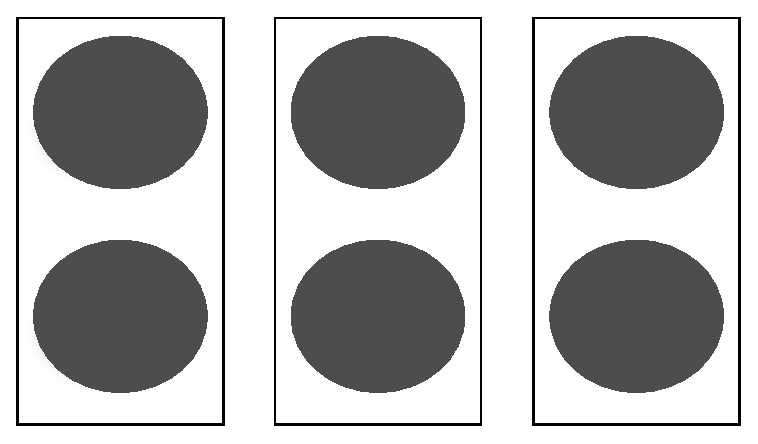
\includegraphics[scale=0.5, bb=0 0 1 1]{warizan1.eps}}
 \put(190,0){\text{図1\ :\ 3つのチーム分け}}
\end{picture}

小学校以来習ってきた割り算というのは,「たくさんあるものを,均等にチーム分けした
時のチーム数を求める演算」だと考えることができます.このイメージを
元に,「集合の割り算」を定義してみましょう.

\Section{商集合}

とはいえ,集合が与えられたとき,いきなり割り算するというのはできません.
「チーム分け」するには何が必要かを考えてみましょう.なお,大学以降では,
集合の要素のことを「元(げん)」というので,これ以降の記事では,要素を元と書くことにします.

\Subsection{同値関係}
チーム分けするためのアイディアは,「同じチームに属する条件」を与えるこ
とです.「同じチームに属している条件」を「同値関係」と言います.「同値関
係」は,以下に定義されるような3つの条件を満たす必要があります.

\begin{defi}[同値関係]
 集合$X$に対し,同値関係$\sim$とは,以下の3つの条件を満たす集合の元の間の関係をいう.
 \begin{enumerate}
  \item(反射律) 全ての$x\in X$に対し,$x \sim x.$
  \item(対称律)  $x\sim y$を満たす全ての$x,y\in X$に対し,$y\sim x$
  \item(推移律) $x\sim y$,$y\sim z$を満たす全ての$x,y,z\in X$に対し,$x\sim
	z$
 \end{enumerate}
\end{defi}
一見,難しそうな定義ですが,よく読めば大したことは言っていません.1つ目の条件は,どんな奴でも自分自身とは同じチーム,
2つ目の条件は,チームメートは逆からみてもチームメート,
3つ目の条件は,チームメートのチームメートはチームメートだと言うことです
(当然成り立ってほしい条件ですよね).


例をいくつかあげてみましょう.
\begin{Ex}
 自然数の集合$\mathbb{N}$において,元の関係$\sim$を
 \[
  n\sim m\Leftrightarrow n-mは2で割り切れる
 \]
 と定めると,これは同値関係です.実際,どんな数$n$についても,$n-n=0$は$2$で割り切れます
 し,$n-m$が$2$で割り切れるなら$m-n$も2で割り切れます.さらに,$n-m,m-l$
 が$2$で割り切れるなら$n-l$も2で割り切れます.今は「$2$」で割り切れると
 しましたが,他の自然数でも上のように定めれば同値関係になることは同様に
 示せます.
\end{Ex}


\begin{Ex}
 実数の集合$\mathbb{R}$において,$\leq(<または=)$で定められる元の関係
 \[
  x\sim y\Leftrightarrow x\leq y
 \]
 は同値関係ではありません.どんな実数$x$に対しても$x\leq x$です
 し,$x\leq y$かつ$y \leq z$ならば$x\leq z$ですから,反射律と推移律は満たしますが,対称律を満たしま
 せん.実際,$x\leq y$だからと言って,$y\leq x$とは限らないからです.
\end{Ex}

同値関係があるとき,同じチームに属している奴らを集めてきたものを,同値類と言います.例
えば,$x\in X$と同値関係にある$X$の元全体($x$が入っているチーム)を,$[x]$で書くことにします.
\[
 [x]=\{y\in X\ |\ x\sim y\}
\]
すると,集合を「チーム分け」する,つまり集合の割り算を定めることができま
す.

\Subsection{商集合の定義}

さて,同値関係が定まると集合の割り算を定義できます.

\begin{defi}[商集合]
 集合$X$とその上の同値関係
 $\sim$に対し,商集合$X/\mathord{\sim}$を以下で定める.
 \[
   X/\mathord{\sim}=\{[x]\ |\ x\in X\}
 \]
\end{defi}

例で感覚を掴みましょう.

 \begin{Ex}{\ } \\
  $X=\{0,1,2,3,4,5,6\}$とします.このとき,$X$に,同値関係$\sim$を,
 \[
  n\sim m\Leftrightarrow n-mが2で割り切れる
 \]
 と定めます.このとき,商集合$X/\mathord{\sim}$は何になるでしょうか.例えば,$1$
  の同値類($1$の入っているチーム)は,$[1]=\{1,3,5\}$, $0$の同値類は,$[0]=\{0,2,4,6\}$となります.こ
  れ以外のチームはありませんから,
  \[
    X/\mathord{\sim}=\{[0],[1]\}=\{\{0,2,4,6\},\{1,3,5\}\}
  \]
であるとわかります.まさに偶数と奇数への「チーム分け」ですよね.$\{0,1\}$
  はチームの代表メンバーであり,数学用語でも「完全代表系」と言います.しかし,
  わり算とはいえ,必ずしも1つ1つのチーム
  の元の数は一致しないことには注意しましょう.
 \end{Ex}

 \Section{様々な商集合の例}
\Subsection{合同式}
  まずは,上の概念をそのまま延長して自然数の集合$\mathbb{N}$に対して,同値
  関係$\sim$を以下で定めてみます.
  \[
   x\sim y\Leftrightarrow x-yが4で割り切れる
  \]
  この同値関係で割った集合$\mathbb{N}/\mathord{\sim}$は,4で割ったあまりでのチーム分けになり
  ます.
  \[
    \mathbb{N}/\mathord{\sim}=\{[0],[1],[2],[3]\}
  \]
  これを図にすると以下のようになります.自然数全体を4つのチームに分け
  てしまったのがよくわかると思います.\\
 \begin{picture}(200,150)(0,0)
   \put(200,20){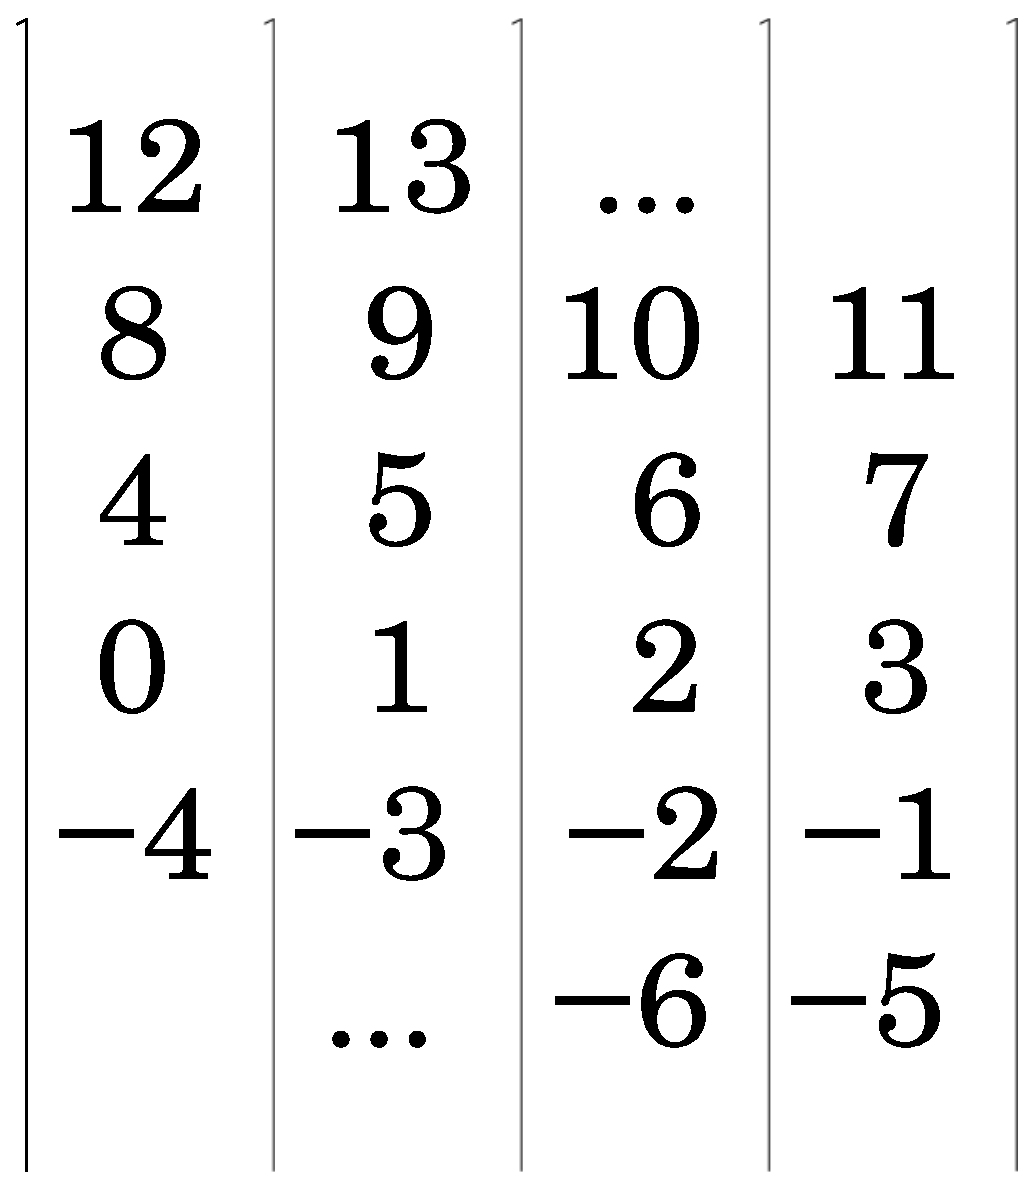
\includegraphics[scale=0.25, bb=0 0 1 1]{warizan2.eps}}
   \put(175,5){\text{図2\ :\ $4$で割ったあまりでチーム分け}}
 \end{picture}
 
  
  合同式を思い出してみましょう.
  \[
   1\equiv5  \mod4
  \]
  などという表記を見たことがあるかもしれませんが,これは,$1$と$5$が上で
  定めた同値
  関係,すなわち$1\sim 5$を示しているに他なりません.
  さらに,もともと$\mathbb{N}$に定まっている足し算,掛け算はそのまま
  $\mathbb{N}/\mathord{\sim}$に遺伝します.つまり,
  \[
   [a]+[b]=[a+b]\hspace{1cm}[a]\times[b]=[a\times b]
  \]
  が成り立つということです.これを使えば,例えば
  \[
   \bigl[15^{30}\bigr]=[15]^{30}=[3]^{30}=\bigl[3^2\bigr]^{15}=[1]^{15}=[1]
  \]
  となり,$15^{30}$がチーム$1$に属する(すなわち,4でわると1あまる)ことがすぐ確かめられます.

\Subsection{ベクトル}
今までは数字を使っていましたが,集合にしたおかげで,もっと概念的なものに
ついても商集合を考えることができます.高校で習うベクトルも,商集合として
考えてみましょう.
$E$を平面(もしくは空間)の有向線分(向きを持った線分,つまり矢印)全体から
なる集合とします.このとき,$E$上の同値関係を,
\[
 v\sim w\Leftrightarrow vとwは平行移動で重なる
\]
と定めます(同値関係になっていることはチェックしてみてください).このとき,
$E/\mathord{\sim}$がまさに平面全体のベクトルを集めた集合になります.この商集合の
 一つ一つの元は「平行移動で重なったら同じベクトルを集めたチーム」になります
 が,この中で原点を始点として持つものを「代表」とすれば,終点の「座
 標」で全てのチームが表せます.これこそがベクトルの「成分表示」なのです.

\Subsection{空間の貼り合わせ}
ベクトルの例からもわかるように,あるものたち(ベクトルの場合は平行移動し
たもの)を{\bf「おんなじものと見たい」「同一視したい」}と
いう気持ちがあるときは,商集合が使われます.数学においては図形同士を,のりで貼
り合わせたいというシーンに多々遭遇しますが,これをキチンと定式化するのも
商集合の大事な役割です.例えば,下の円と直線を黒点の部分で貼り合わせてみましょう.

\begin{picture}(150,100)(0,0)
 \put(150,10){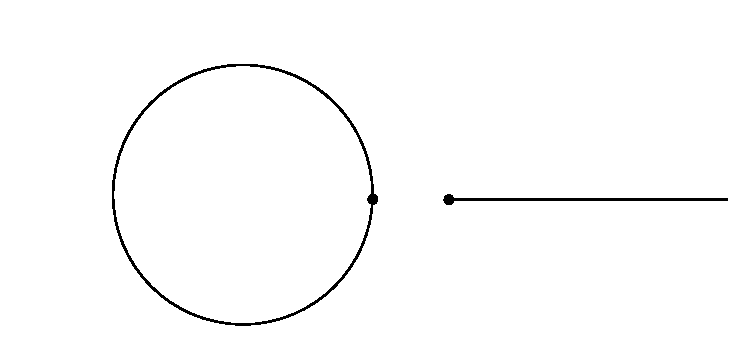
\includegraphics[scale=0.5, bb=0 0 1 1]{warizan4.eps}}
\end{picture}

このとき,二つの図形の点の集まりを一つの集合$X$だと考え,$A$を2つの黒点からなる集合として,以下のよう
な同値関係を定めます(同値関係になっていることはすぐ確かめられます).
\[
 x\sim y\Leftrightarrow 
			x,y \in Aまたは
			x=y 
\]
つまり,$A$に入っていない点たちは,その点1点からなるチームに,$A$に入っ
ている点たちはまとめて一つのチームにしてしまいます.そうすれば,チーム全
体の集合$X/\mathord{\sim}$は,まさに,二つの図形を貼り付けたものになっていることがわかりま
す.
このような貼り付けにより作られる図形の一つをみてみましょう.正方形の辺を貼り付けて立体を作るということを考えてみます.図の黒点同士のように,左側の辺と右
側の辺,上と下も同様に,同じ方向に貼り付けると,右のように浮き輪の形の図
形が出来上がります.これは(2次元)トーラスといい,数学の様々な場面に登場
します.

\begin{picture}(400,120)(0,0)
 \put(40,10){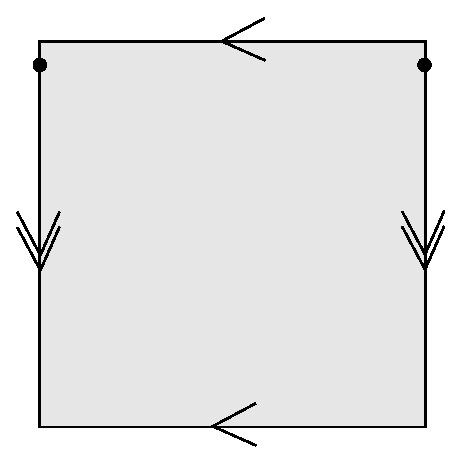
\includegraphics[scale=0.5, bb=0 0 1 1]{warizan3.eps}}
 \put(150,55){\text{\huge $\Rightarrow$}}
 \put(175,30){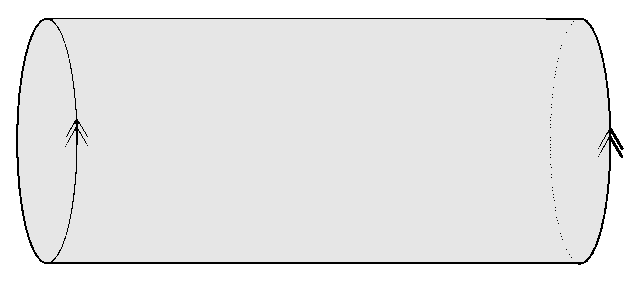
\includegraphics[scale=0.5, bb=0 0 1 1]{warizan5.eps}}
 \put(325,55){\text{\huge $\Rightarrow$}}
 \put(350,30){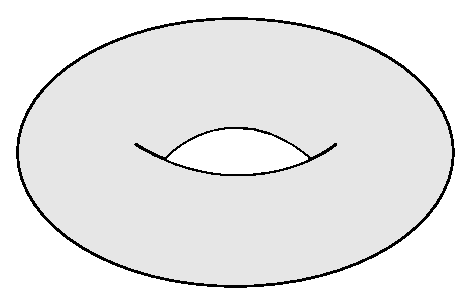
\includegraphics[scale=0.5, bb=0 0 1 1]{torus.eps}}
 \end{picture}

ちなみに,貼り付けかたを一つだけ逆にすればクラインの壺,二つとも逆に
すると二次元射影空間と呼ばれる図形になります(想像できますか?).\\
二次元球面(地球の表面)は地球上の地図を貼り合わせて構成できますし,多くの図形は
貼り合わせによって構成が可能です.大雑把に言って,このように直線や平面な
どまっすぐな空間を貼り合
わせて作られる図形のことを数学では多様体と呼び,古くから研究されてきた対
象です.

\Subsection{商ベクトル空間*}
ここで扱う例は,大学1年生で習うベクトル空間の概念なので,知らない人は
飛ばしてもらって結構です.\\

ここまでの概念がわかってしまえば,大学1年生の線形代数での1つの難所である
商空間は簡単に定義できます.

\begin{defi}
 ベクトル空間$V$と部分空間$W$に対し,$V$上の同値関係を,
 \[
  v_1\sim v_2\Leftrightarrow v_1-v_2\in W
 \]
 と定義する.$V/\mathord{\sim}$を,部分空間$W$による$V$の商空間といい,$V/W$で表す.
\end{defi}

これだとイメージしにくいかもしれませんが,$v_1$の同値類$[v_1]$は
$v_1+w\ (w\in W)$
と書けるものな訳ですから,$W$の元だけずれているものは全て同じチームなの
です.絵で描けば,以下のようになります.まず,部分空間とは,原点を通るまっ
すぐな空間ですから,$V$と$W$の図は以下のようになります.\\
\begin{picture}(400,150)(0,0)
 \put(150,10){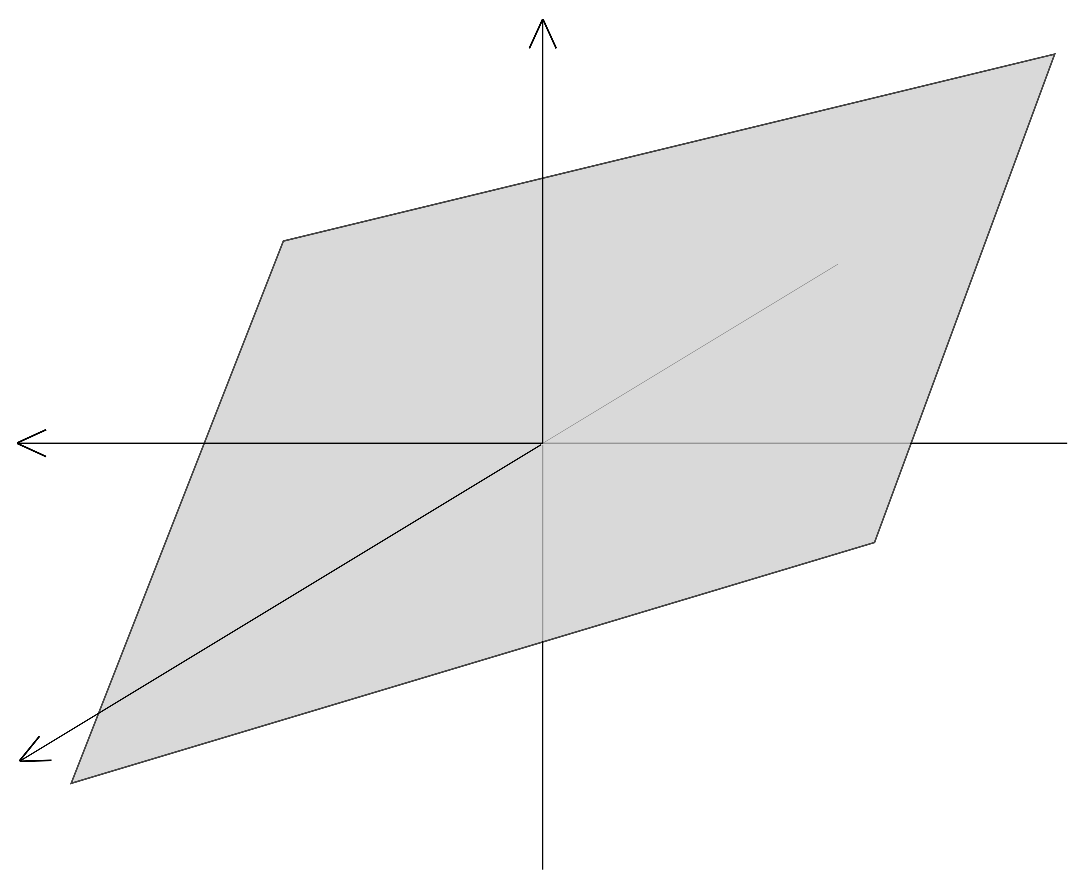
\includegraphics[scale=0.4, bb=0 0 1 1]{warizan6.eps}}
 \put(260,100){\text{$W$}}
\end{picture}

この空間$W$全てが同じチームとなりますので,チームは以下
のようにならんでいることがわかります.つまり,商空間とは,この1枚1枚のチームの全体となるの
です.完全代表系は,$W$と原点のみにおいて交わる直線と平面たちの交点となり
ます(完全代表系の取り方は無限通りあります).つまり,商空間$V/W$はこの直線と同
一視できるのです.スカラー倍や足し算については合同式のときと同じく商集合に遺
伝することが示せるので,$V/W$もベクトル空間となることがわかります.
イメージとしては,商空間$V/W$は$V$を図の直線に向かって潰した空間というこ
とになります.潰した時,$W$は原点に潰れるわけですから,$V$において,$W$
の成分を全て$0$と同一視したものだとも言えます.


\begin{picture}(400,150)(0,0)
 \put(150,10){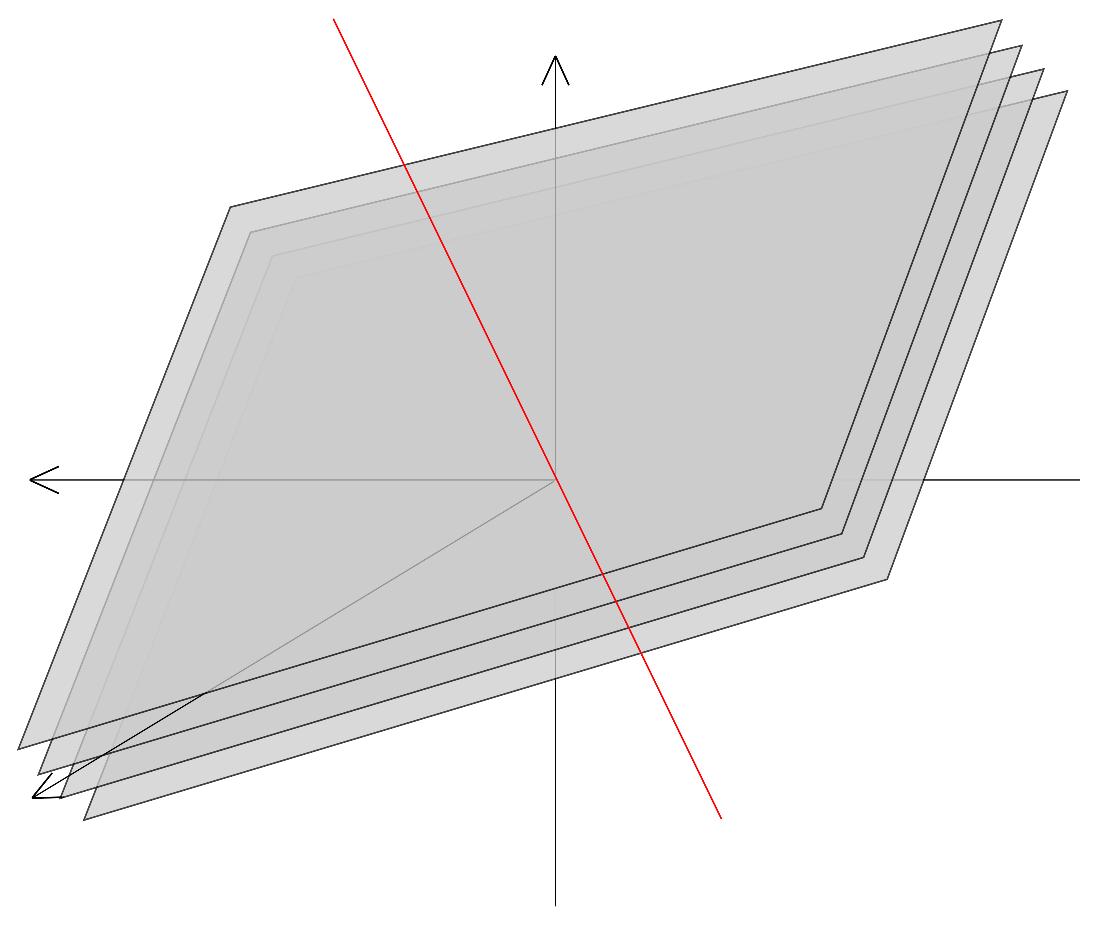
\includegraphics[scale=0.4, bb=0 0 1 1]{warizan7.eps}}
\end{picture}
\Section{数の構成}

さて,ここからは応用編です.唐突ですが,「整数,有理数,実数とは何か」と聞かれ
たとき,何て答えるでしょうか.「え,そりゃあ,$-1$とか分数とかでしょ?」
とか答えられても,あくまでそれは例にすぎません.「自然数の集合
$\mathbb{N}$と足し算,掛け算しか知らない」と仮定
して,整数の集合$\mathbb{Z}$や有理数の集合$\mathbb{Q}$,実数の集合$\mathbb{R}$を自然数のみを用いて構成してみ
ることにします.(今回は,自然数の存在は暗に認めています.公理的集合論の
立場では自然数は無限公理を満たす最小の集合として存在を保証しているのですが,今回は解説しないことにし
ます.)\footnote{以下の話の厳密な証明が知りたい場合,\cite{mathpdf}を参照してください.}

\Subsection{自然数から整数}

さて,自然数から整数を構成することを考えてみましょう.一番簡単なアイディ
アは,プラスパートとマイナスパートの自然数を作るということです.$(a,b)$と書
いたとき,1つめの項はプラス,2つ目の項はマイナスに当たると考えてみましょ
う.例えば,$(2,0)$を$2$に当たる数として,$(0,3)$を$-3$に当たる数として定めるわけです.そして,2つの数
の足し算を$(2,0)+(0,3)=(2,3)$と定めます.$(2,3)$はプラスパートとマ
イナスパートがそれぞれ$2,3$ですから,$-1$を表していると考えます.これで一見,うまくいっ
たかのように見えますが,これだと$(2,3)$と$(0,1)$が同じ数字を表しているた
め,”ダブり”が生じています.$(2,3)$と$(0,1)$を同じものと見たい,同一視し
たい.こんな時こそ商集合の出番です.


\begin{defi}[整数]
 自然数を二つ並べた集合$\mathbb{N}^2=\{(a,b)\ |\ a,b\in
\mathbb{N}\}$を考え,$\mathbb{N}^2$上に同値関係
\[
 (a,b)\sim(c,d)\Leftrightarrow a+d=b+c
\]
と定め,この同値関係による商集合$\mathbb{N}/\mathord{\sim}$を整数$\mathbb{Z}$と
 定める.
 さらに,$\mathbb{Z}$上の加法と乗法を,
 \[
  [(a,b)]+[(c,d)]=[(a+b,c+d)]\hspace{1cm}[(a,b)]\times[(c,d)]=[(ac+bd,ad+bc)]
 \]
 と定める\footnote{本当は,これで矛盾なく定まっていることをチェックしなければいけません.つまり,$(a,b)\sim(a',b')$のとき,\[(a+c,b+d)\sim(a'+c,b'+d)\hspace{1cm}(ac+bd,ad+bc)\sim(a'c+b'd,a'd+b'c)\]であることを示す必要があります.もしこうでなければ,足し算や掛け算の結果が,チームの代表メンバーの選び方によって違う結果になってしまい,矛盾してしまうからです.一つ目だけチェックすれば,$a+b'=a'+b$より$(a+c)+(b'+d)=(a'+c)+(b+d)$ですからうまくいっています(二つ目もチェックしてみましょう).このようにうまく定まっていることを,数学では,well-definedと言います.}
\end{defi}

例えば,$2+1=3+0$ですから,$[(2,3)]=[(0,1)]$だとわかりま
す.
掛け算はちょっと技巧的ですが,これでうまくいっていることがわかります.例
えば,正の数同士は,$[(n,0)]\times[(m,0)]=[(nm,0)] $と,今までと全く同じ
演算であることがわかります.また,$[(n,0)]\times[(0,m)]=[(0,nm)]$や,
$[(0,n)]\times[(0,m)]=[(nm,0)]$などから,プラスかけるマイナスがマイナ
ス,マイナスかけるマイナスがプラスであることも説明できます.\\
最後に,$[(x,0)]$を$x$とかき,$[(0,x)]$を$-x$を書くことにすれ
ば,今まで使っていた表記と合致します.


\Subsection{整数から有理数}

さて,今度は有理数を構成してみましょう.さっきのアイディアをそのまま借用
して,分母パートと分子パートを並べて書いてみることにします.つまり,
$(a,b)$と書いたとき,$\ds\frac{a}{b}$を表すとしてみます.しかし,分数と
いうのは,小学校以来,約分しても同じ,だったわけですから,例えば$(2,4)$
と$(1,2)$は同じものであってほしいわけです.そこで,商集合を使って同一視
してみます.

\begin{defi}[有理数]
$\mathbb{Z}\times(\mathbb{Z}-\{0\})=\{(a,b)\ |\
 a\in\mathbb{Z},b\in\mathbb{Z}-\{0\}\}$上に同値関係
 \[
  (a,b)\sim(c,d)\Leftrightarrow ad=bc
 \]
 と定め,この同値関係による商集合
 $\mathbb{Z}\times(\mathbb{Z}-\{0\})/\mathord{\sim}$を有理数$\mathbb{Q}$と定める.
 さらに,$\mathbb{Q}$上の加法と乗法を,
 \[
  [(a,b)]+[(c,d)]=[(ad+bc,bd)]\hspace{1cm}[(a,b)]\times[(c,d)]=[(ac,bd)]
 \]
 と定める\footnote{これもwell-definedであることをチェックする必要があります.示してみてください.}.
\end{defi}

$\sim$の同値関係は,外項と内項の積が等しい,つまり,$a:b=c:d$を表していますから,同じ分数を1チームにまとめていることがわかります.\\
さて,定義から,$[(1,1)]$はどんな数とかけても相手を変えない,自然数の''1''に当たる数だとわかります.また,$[(0,1)]$は,どんな数とかけても$[(0,1)]$になり,どんな数と足し算しても相手を変えない,自然数の''0''に当たる数だとわかります.\\
また,
\[
 [(a,b)]\times[(b,a)]=[(ab,ab)]=[(1,1)]
\]
ですから,$[(a,b)]$に,$[(b,a)]$をかけると1になることがわかります.
ということは,
\[
 [(c,d)]=[(a,b)]\times([(b,a)]\times[(c,d)])
\]
ですから,
\[
 [(c,d)]/[(a,b)]=[(b,a)]\times[(c,d)]
\]
となり,小学校以来やってきた,分数の割り算は分母と分子をひっくり返してかけるということも正当化できます.

最後に,$(a,b)$を$\ds\frac{a}{b}$と書く\footnote{ちなみに,$\ds\frac{a}{b}$は日本語では「$b$分の$a$」と読みますが,英語では逆で,''$a$ over $b$''と読みます.}ことにすれば,今まで使っていた表記と合致します.

\Subsection{有理数から実数}

さて,最後に実数を作ってみましょう.これはかなり困難です.実数の構成には,代表的なものでDedekind cutによるものと,有理数の完備化の二つがあるのですが,今回は有理数の完備化を解説したいと思います.
\begin{defi}[Cauchy列]
 数列$\{a_n\}$がCauchy列であるとは,以下のことを言う.
 \[
  \forall \varepsilon >0 \ \exists N\  {\rm such\ that}\ n,m>N \Rightarrow |a_n-a_m|<\varepsilon
 \]
\end{defi}
一見ギョッとするような定義ですが,簡単に言えば,コーシー列とは,「二項間の差がどんどん小さくなっていくような数列」のことです.
さて,ここで,次のような問題を考えて見ましょう.
\begin{center}
 Cauchy列は収束するでしょうか?
\end{center}
答えは,実数列なら○,有理数列なら×です.数学用語でこの性質を「完備性」と言います.有理数は完備ではないのです.例えば,有理数で$\sqrt{2}$に近づくような数列を考えてみれば,もちろん二項の差は縮まっていきますが,肝心の収束先の$\sqrt{2}$が有理数ではないですから,「有理数の中では」収束しません.このことに着目して,有理数から実数を作ります.具体的には,
\begin{center}
  $\sqrt{2}$ に収束する有理数列を $\sqrt{2}$ だと定義する
\end{center}
です.数列と $\sqrt{2}$ を同じと見るなんてかなり気持ち悪いですが,一応定義はできるわけです.とはいっても,$\sqrt{2}$に収束する有理数列はいっぱいあります.そこで,商集合の考え方を使って,$\sqrt{2}$に収束する数列を1チームにしてしまえば良いのです.
\begin{defi}[実数]
$\mathcal{C}$を有理数のCauchy列全体からなる集合とし,$\mathcal{C}$上の同値関係を,
 \[
 \{a_n\}\sim\{b_n\}\Leftrightarrow \forall\varepsilon\  \exists N\  {\rm such\ that}\ n>N\Rightarrow |a_n-b_n|<\varepsilon
 \]
 と定め\footnote{これが同値関係であることは非自明ですが,ここでは省略します.},この同値関係による商集合$\mathcal{C}/\mathord{\sim}$を実数$\mathbb{R}$と定める.さらに,$\mathbb{R}$上の加法と乗法を,
 \[
  [\{a_n\}]+[\{b_n\}]=[\{a_n+b_n\}]\hspace{1cm}[\{a_n\}]\times[\{b_n\}]=[\{a_nb_n\}]
 \]
 と定める.\footnote{これがwell-definedであることも非自明ですが,ここでは省略します.}
\end{defi}

上のように定めれば$\{a_n\}\sim\{b_n\}$であれば,$\{a_n\}$と$\{b_n\}$が同じ値に近づいていくことがわかります.
本当は,$\mathbb{R}$が満たすべきたくさんの性質をここから示さなければいけないのですが,今回の主題はそこではないので,詳しくは参考文献を見てみてください.

このように,存在が当たり前だと思っていた整数や有理数や実数,そしてそのたくさんの性質は,商集合のアイディアに支えられているのです.\footnote{実は複素数も,商集合を用いて$k[X]/(X^2+1)$などと定義できるのですが,今回は紙面の関係上,省略します.}


\Section{応用**}
最後に,少しだけ応用をみてみます.
 \Subsection{等質空間}
群構造をもつ可微分多様体で群の積演算$(a,b)\mapsto ab$と逆演算$a\mapsto a^{-1}$が可微分であるものをLie群と言います(群と多様体のあいのこです).例えば,一般線形群$GL(n,\mathbb{R})$や特殊線形群$SL(n,\mathbb{R})$,特殊直交群$SO(n)$などはLie群になっています.

さて,Lie群$G$がある多様体$M$に推移的に作用していることを考えてみましょう.推移的,というのは全ての点同士があるLie群の元の作用で写りあえるという意味です.全射群準同型$G\rightarrow \rm{Diff}(M)$があると言ってもいいです.
例えば,球面$S^n$,上半平面$H$には,
\begin{eqnarray*}
SO(n+1)&\rightarrow & {\rm Diff}(S^{n})\hspace{1cm}A\mapsto (p\mapsto Ap)  \\
SL(2,\mathbb{R})&\rightarrow & {\rm Diff}(H)\hspace{1cm}\left(\begin{matrix}a&b\\c&d\end{matrix}\right)\mapsto\left(z\mapsto\frac{az+b}{cz+d} \right) 
 \end{eqnarray*}
のように,Lie群が推移的に作用しています.
この時,ある一点$p$の群作用による行き先(軌道)は,推移的であるという仮定から全体を覆うわけですが,作用させても動かない$G$の元があるかもしれません.これを集めたもの,
\[
 H=\{g\in G\ |\ gp=p\}
\]
を$G$の一点$p$の固定部分群と言います(定義より閉部分群になります).
この$H$たちをチームにして, 点$p$と同一視すれば,作用させている空間との1対1対応ができます.
すなわち,
\[
 G/H\simeq M\hspace{1cm}[g]\mapsto gp
\]
となるわけです.

ここで,左辺の$G/H$とは,$G$を,$g_1\sim g_2\Leftrightarrow g_1g_2^{-1}\in H$という同値関係で割ったもので,$G$の部分群$H$による商群と呼ばれます.特に,Lie群をその中の閉部分群で割った商群$G/H$には多様体構造が定まることが知られており,上の同型は微分同相であることが示せます.

このように,Lie群が推移的に作用している多様体は,必ずLie群の商の形で書くことができます.このような多様体を等質空間と言います.

\begin{Ex}[球面]
 $SO(n+1)$の作用による球面$S^n$上のある1点$(0,0,0,\cdots,0,1)$の固定部分群は,
 \[
\left\{
\left(
\begin{array}{ccc:c}
&&&\\
&\mbox{\smash{\huge\textit{A}}}&&{{0}}\\
&&&\\ \hdashline
&0&&1
\end{array}
\right) \middle|\ A\in SO(n) \right\}\simeq SO(n)
 \]
よって,$S^n\simeq SO(n+1)/SO(n)$となります.
\end{Ex}

\begin{Ex}[上半平面]
$SL(2)$の作用による上半平面$H$上のある1点 $i$ ($=\sqrt{-1}$) の固定部分群は,
 \[
  \frac{ai+b}{ci+d}=i\Leftrightarrow a=d,\ b=-c
 \]
より,
 \[
  \left\{\left(\begin{matrix}
   a&b\\c&d
  \end{matrix}\right)\in SL(2,\mathbb{R})\ \middle|\  a=d,b=-c\right\}\simeq SO(2)
 \]
よって,$H\simeq SL(2,\mathbb{R})/SO(2)$となります.$H$は複素多様体ですが,実Lie群の商でかけます.
\end{Ex}

この表示の一つのメリットは,ある1点に定めた幾何構造を全体に写すことにあります.
$G/H$の形で書いた場合,当然,原点の同値類$[e]$があります.
これについて
\begin{Lemma}\label{l4}
  $G/H$を等質空間とする.集合として,次の同型がある.
 \[
  (\bigotimes^rT_{[e]}M\otimes\bigotimes^sT^*_{[e]}M)^H\simeq (\Gamma(M,\bigotimes^rTM\otimes\bigotimes^sT^*M))^G
 \]
 ただし,左は,$\Ad(H)$不変なテンソルの元,右辺は$M$からベクトル束への左作用の微分${L_{G}}_*$不変な切断である.
 \end{Lemma}
表示は仰々しいですが,例えば,$r=1,s=0$とすれば,$H$不変な接空間のベクトルと,$G$不変なベクトル場が1対1に対応していることがわかりますし,$r=0,s=2$とすれば,$H$不変な接空間上の内積と,$G$不変な計量,$H$不変な複素構造と$G$不変な概複素構造が1対1に対応することがわかります.\\
他にも,等質空間上では測地線をLie代数からLie群への指数写像でかけたり,曲率テンソルが,Lie括弧でかなりシンプルにかけたりなど,計算できる具体例を豊富に提供してくれます.


\Subsection{Clifford-Klein形}
Riemannの一意化定理の一般化である,Klein-Poincar\'e-Koebeの一意化定理より,Riemann面の普遍被覆は,上半空間$H$,複素数$\mathbb{C}$,複素射影空間$\mathbb{P}^1$のいずれかに正則同値になります.また,特に,種数が2以上のコンパクトRiemann面は,上半平面を,Fuchs群と呼ばれる$\rm{Aut}(H)$の離散部分群$\Gamma$で割って作られます.$H$自体は上で見たように$SL(2,\mathbb{R})/SO(2)$とかけますから,コンパクトRiemann面は,$\Gamma\backslash SL(2,\mathbb{R})/SO(2)$という$SL(2,\mathbb{R})$を2回割ったものとして書くことができます.一般に,$G/H$に固有不連続かつ自由に作用する$G$の離散部分群$\Gamma$が存在すれば,等質空間$G/H$をさらに割った$\Gamma\backslash G/H$を考えられます.これをClifford-Klein形といい,等質空間より豊富な例を含む広いクラスとして,現在も研究されています.

{\bf 終わりに}\\
たくさんの例を「割り算」というテーマでざっくばらんに解説してみました.何を隠そう,この集合の割り算という概念を理解するのに僕自身苦労したので,あえて書いて見ました.数学というと,「イメージではなく,論理的にのみ考える学問」と考えられがちな気がします.論理ももちろん大事ですが,決して論理だけではなく,むしろ,「イメージをいかに数式という形で正確に伝えられるか」というモチベーションで研究が進むことも多いと思います.高校や大学で難しい概念に出会ったときは,ただ定義を眺めるだけではなく,様々な例を見ながら,どういう気持ちで概念が生まれているのかを考えて見るといいと思います.

\begin{thebibliography}{99}
\bibitem{mathpdf} 数の構成 自然数から複素数まで \url{http://mathematics-pdf.com/pdf/construction_of_numbers.pdf}
\bibitem{hel} S.Helgason.Differetntail Geometory and Symmetric Spacees.AMS Chelsea Publishing,2001
\bibitem{sat} 佐武一郎.線型代数学.裳華房,数学選書1,1974
\bibitem{mat} 松坂和夫.集合・位相入門.岩波書店,1968
\bibitem{kob} 小林俊行.数学の最先端21世紀への挑戦.vol1.Springer,2001
\end{thebibliography}

\clearpage
\Section{圏論が分かる4コマ漫画2(小林)}
\begin{center}
\includegraphics[width=0.9\textwidth]{kobaken2.png}
\end{center}

\documentclass{ltjsarticle}
\usepackage{amsmath,amssymb,amsthm}
\usepackage{mathcomp}
\usepackage{graphicx,color}
\usepackage{verbatim}
\usepackage{tikz}
\usepackage{luatexja-ruby}
\usepackage[pdfusetitle]{hyperref}
\title{たのしい複素積分}
\author{荒田 実樹}

\usetikzlibrary{arrows.meta,decorations.pathreplacing,decorations.markings,shapes.misc,patterns}

\newcommand{\Natural}{\mathbf{N}}
\newcommand{\Integer}{\mathbf{Z}}
\newcommand{\Real}{\mathbf{R}}
\newcommand{\Complex}{\mathbf{C}}
\newcommand{\ImagI}{i}%{\sqrt{-1}}%{\mathbf{i}}
\newcommand{\innerProd}[2]{\left\langle #1,#2\right\rangle}
\newcommand{\norm}[1]{\left\lvert #1\right\rvert}
\newcommand{\abs}[1]{\left\lvert #1\right\rvert}
\DeclareMathOperator{\RealPart}{Re}
\DeclareMathOperator{\ImagPart}{Im}
\DeclareMathOperator{\Residue}{Res}

\theoremstyle{definition}
\newtheorem{theorem}{定理}
\newtheorem{lemma}[theorem]{Lemma}
\newtheorem*{lemma*}{Lemma}
\newtheorem{proposition}[theorem]{Proposition}
\newtheorem*{proposition*}{Proposition}
\newtheorem{cor}[theorem]{Corollary}
\newtheorem*{cor*}{Corollary}
\newtheorem{fact}[theorem]{Fact}
\newtheorem*{fact*}{Fact}
\newtheorem{definition}{Definition}
\newtheorem*{definition*}{Definition}

\theoremstyle{remark}
\newtheorem{remark}[definition]{Remark}
\newtheorem*{remark*}{Remark}
\newtheorem{claim}{Claim}
\newtheorem*{claim*}{Claim}
\newtheorem{example}{例}
\newtheorem*{example*}{Example}
\newtheorem{exercise}[example]{問題}

\begin{document}
%\maketitle

\Chapter{たのしい複素積分(荒田)}

\Section{はじめに}

数ヶ月前のことですが,複素積分で遊べるWebページを作りました.
以下のURLからアクセスできます.URLを打ち込むのが面倒な人はQRコードを読み取ってください.
あるいは,「たのしい複素積分」でググったら出てくるかもしれません.

\begin{center}
\url{http://d-poppo.nazo.cc/math/singularity/} \\
\includegraphics[width=3cm]{arata-qrcode.eps}
\end{center}

この記事では,複素積分ってなにそれおいしいの?という人のために複素解析のさわりを紹介します.
諸概念の厳密な定義とか定理の証明とかはここではしないので,複素解析の教科書を読んでください.

複素解析の教科書としては,Ahlforsによる教科書\cite{Ahlfors} が定番でしょう.
邦訳\cite{Ahlfors-ja} もあります.
高校生や大学初年度向けの入門書として,『複素数の世界』\cite{Ueno} も挙げておきます.
図書館で探してみると良いでしょう.

以下では,読者は,複素数の基本的な性質及び,実数の微積分についてはある程度知っているものとします.
%高校生 $+\alpha$ ぐらいの知識で読めるといいな

\newcommand{\exampleautorefname}{例}

\Section{複素関数}
複素数に複素数を対応させる関数 $f\colon\Complex\to\Complex$ を複素関数と呼びます.
正確には,複素平面全体で定義されている必要はなくて,複素平面の一部分で定義されていれば複素関数と呼びます(\autoref{example:1/z} など).

複素数は2つの実数の組と思えますが,それと同じように,複素関数 $f(z)$ は,2変数の実関数 $u(x,y)$, $v(x,y)$ を組み合わせたものと見ることもできます.
\[f(x+\ImagI y)=u(x,y)+\ImagI v(x,y)\]

% 図
%\begin{center}
%  \begin{tikzpicture}
%    \draw [-{Stealth}] (-2,0) -- (2,0);
%    \draw [-{Stealth}] (0,-2) -- (0,2);
%    \draw plot [smooth cycle, tension=1] coordinates {(-1,-0.9) (-0.3,-0.8) (0.7,-0.9) (1.3,0.3) (0.8,1) (0.1,0.8) (-0.7,1.2) (-1,0.3) (-0.9,-0.2)};
%  \end{tikzpicture}
%\end{center}

いくつかの複素関数について,その実部 $u(x,y)$ と虚部 $v(x,y)$ を見てみましょう.

\begin{example}
  $f(z)=z^2+1$ という関数について,
  %\[
  %f(x+\ImagI y)
  %=(x+\ImagI y)^2+1
  %=x^2+2\ImagI xy-y^2+1
  %\]
  %より
  \[u(x,y)=x^2-y^2+1, \quad v(x,y)=2xy.\]
  %である.
\end{example}

\begin{example}
  指数関数 $f(z)=\exp z$ について,%の $u$, $v$ は
  \[u(x,y)=e^x\cos y, \quad v(x,y)=e^x\sin y.\]
\end{example}

\begin{example} \label{example:1/z}
  複素数の逆数をとる関数 $f(z)=\frac{1}{z}$ は,複素平面から原点 $0$ を除いた部分で定義される.
  この関数について,実部と虚部は
  \[u(x,y)=\frac{x}{x^2+y^2}, \quad v(x,y)=-\frac{y}{x^2+y^2}.\]
\end{example}

\begin{example}
  複素数の実部をとる関数 $f(z)=\RealPart z$ について,
  \[u(x,y)=x, \quad v(x,y)=0.\]
\end{example}

\begin{example}
  複素共役をとる関数 $f(z)=\bar{z}$ について,
  \[u(x,y)=x, \quad v(x,y)=-y.\]
\end{example}


\Section{複素微分と正則関数}
\newcommand{\pdiff}[2]{\frac{\partial #1}{\partial #2}}

複素積分の話に入る前に,複素関数の微分を定義しておきます.
点 $z=z_0$ のまわりで定義された複素関数 $f$ について,極限
\[\lim_{h\to 0} \frac{f(z_0+h)-f(z_0)}{h}\]
が存在するとき, $f$ は点 $z_0$ で複素微分可能であるといいます.
このとき,$f$ の $z=z_0$ における微分係数 $f'(z_0)$ を,その極限値
\[f'(z_0):=\lim_{h\to 0} \frac{f(z_0+h)-f(z_0)}{h}\]
として定義します.
定義域のいたるところで複素微分できる関数を\ruby{正則}{せいそく}関数(holomorphic function)と呼びます.

一見すると変数が実数のときの微分と同じ定義ですが,実数の場合は $h$ が左から近づくか右からかぐらいしか $0$ への近づき方がなかったのに対し,ここでの $h$ は上下左右どの方向からでも $0$ に近づいても良いという点が違います.
このことによって,複素関数が微分できるという条件は,対応する実数の関数 $u$, $v$ が(実数の意味で)微分可能である,という条件よりも強い条件となっています.

% 近づき方の図
\begin{center}
  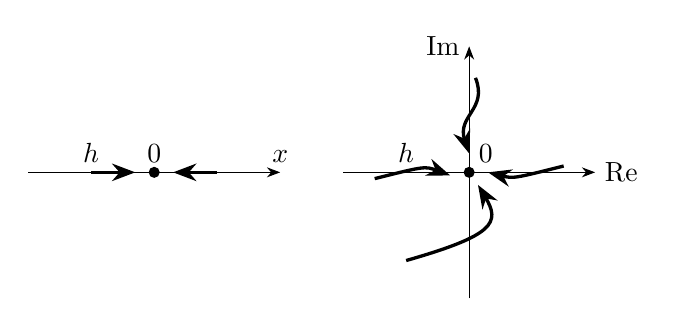
\begin{tikzpicture}[x=0.8cm,y=0.8cm]
    \begin{scope}[xshift=-2cm]
      \draw [-{Stealth}] (-2,0) -- (2,0) node [above] {$x$};
      \draw [-{Stealth},very thick] (-1,0) -- (-0.3,0);
      \fill (0,0) circle (2pt) node [above] {$0$};
      \draw [-{Stealth},very thick] (1,0) -- (0.3,0);
      \node [above] at (-1,0) {$h$};
    \end{scope}
    \begin{scope}[xshift=2cm]
      \draw [-{Stealth}] (-2,0) -- (2,0) node [right] {Re};
      \draw [-{Stealth}] (0,-2) -- (0,2) node [left] {Im};
      \fill (0,0) circle (2pt) node [above right] {$0$};
      \begin{scope}[-{Stealth},very thick]
        \draw (1.5,0.1) .. controls (0.7,-0.1) .. (0.3,0);
        \draw (-1.5,-0.1) .. controls (-0.7,0.1) .. (-0.3,-0.05);
        \draw (0.1,1.5) .. controls (0.3,1) and (-0.2,0.9) .. (0,0.3);
        \draw (-1,-1.4) .. controls (0.4,-1) and (0.5,-0.8) .. (0.14,-0.2);
      \end{scope}
      \node [above] at (-1,0) {$h$};
    \end{scope}
  \end{tikzpicture}
\end{center}

先に書いた例の関数はどれも実数の意味では微分できます($u$, $v$ が全微分可能)が,複素微分できるもの(正則なもの)は
\[z^2+1, \quad \exp z, \quad \frac{1}{z}\]
だけです.
$\RealPart z$ と $\bar{z}$ は複素数の意味での微分ができません.
$h\to0$ の近づけ方によって極限の値が変わってしまうのです.

\Section{複素積分の定義}

いよいよ,複素関数の積分を定義します.
実数の積分(定積分)では,積分する区間の始点と終点を決めれば積分が決まりましたが,複素積分では,始点と終点だけではなくてそれらを結ぶ「道」(積分路)を指定してやる必要があります.

\begin{center}
  \begin{tikzpicture}[x=0.8cm,y=0.8cm]
    \draw [-{Stealth}] (-2,-0.8) -- (2,-0.8);
    \draw [-{Stealth}] (-0.6,-2) -- (-0.6,2);
    \fill (-1,0) circle (2pt) node [above left] {始点};
    \fill (1,0.2) circle (2pt) node [below right] {終点};
    \draw [postaction={decorate},decoration={markings,mark=at position .5 with {\arrow{Stealth}}},thick]
      (-1,0) .. controls (0,-1) and (0.1,1.2) .. (1,0.2)
      node [midway,above left] {$\gamma$};
  \end{tikzpicture}
\end{center}

% 図
この道を
%$\gamma\colon[0,1]\to\Complex$
$\gamma(t) \ (0\le t\le 1)$
とパラメーター表示\footnote{パラメーターの区間は別に $[0,1]$ でなくてもいいのですが,ここでは $[0,1]$ としておきます.}したとき,
道 $\gamma$ に沿った $f(z)$ の積分(線積分とも言う) $\int_\gamma f(z)dz$ を
\[\int_\gamma f(z)dz:=\int_0^1 f(\gamma(t))\gamma'(t)dt\]
によって定めます.
右辺は, $f(\gamma(t))\gamma'(t)$ を実部と虚部に分けてやって,それぞれ実数の積分として計算します.

%この定義の見た目は,実数の置換積分の公式に似ています.

\begin{example}
  図のような線分に沿って $f(z)=z^2$ を積分してみましょう.
  \begin{center}
    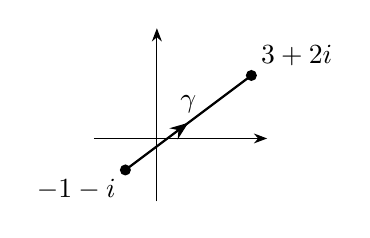
\begin{tikzpicture}[x=0.4cm,y=0.4cm]
      \draw [-{Stealth}] (-2,0) -- (3.5,0);
      \draw [-{Stealth}] (0,-2) -- (0,3.5);
      \fill (-1,-1) circle (2pt) node [below left] {$-1-i$};
      \fill (3,2) circle (2pt) node [above right] {$3+2i$};
      \draw [postaction={decorate},decoration={markings,mark=at position .5 with {\arrow{Stealth}}},thick] (-1,-1) -- (3,2) node [midway,above] {$\gamma$};
    \end{tikzpicture}
  \end{center}
  積分路のパラメーター表示を
  \[\gamma(t)=(-1-i)(1-t)=(3+2i)t=(4+3i)t-1-i\]
  とおくと,
  \begin{align*}
    \int_\gamma z^2dz
    &=\int_0^1 \gamma(t)^2\gamma'(t)dt \\
    &=\int_0^1 ((4+3i)t-1-i)^2\cdot(4+3i) dt \\
    &=-\frac{11}{3}+16i
  \end{align*}
  となります(途中の計算は省略しました).
\end{example}

\begin{example}
  関数 $f(z)=\frac{1}{z}$ を $1$ から $-1$ まで,2通りの積分路(図の壱と弐)で積分してみましょう.
  この関数は $z=0$ で定義されないので,積分路は $z=0$ を通らないように選ぶ必要があります.

  \begin{center}
    \begin{tikzpicture}
      \draw [-{Stealth}] (-2,0) -- (2,0);
      \draw [-{Stealth}] (0,-2) -- (0,2);
      \fill (-1,0) circle (2pt) node [above left] {$-1$};
      \fill (1,0) circle (2pt) node [above right] {$1$};
      \node [draw=black,cross out] at (0,0) {};
      %\draw (-2pt,-2pt) -- (2pt,2pt) (2pt,-2pt) -- (-2pt,2pt);
      \node (0,0) [above right] {$0$};
      \begin{scope}[decoration={markings,mark=at position .5 with {\arrow{Stealth}}},thick]
        \draw [postaction={decorate}]
          (1,0) arc [start angle=0, end angle=180, radius=1]
          node [midway,above left] {壱};
        \draw [postaction={decorate}] (1,0) arc [start angle=0, end angle=-180, radius=1]
          node [midway,below right] {弐};
      \end{scope}
    \end{tikzpicture}
  \end{center}

  壱($z=0$ の上側を通る):
  $\gamma(t)=e^{\pi i t}$
  \[
  \int_\gamma \frac{dz}{z}
  =\int_0^1 \frac{\pi i e^{\pi i t}}{e^{\pi i t}} dt
  =\int_0^1 \pi i dt
  =\pi i
  \]

  弐($z=0$ の下側を通る):
  $\gamma(t)=e^{-\pi i t}$
  \[
  \int_\gamma \frac{dz}{z}
  =\int_0^1 \frac{-\pi i e^{-\pi i t}}{e^{-\pi i t}} dt
  =-\int_0^1 \pi i dt
  =-\pi i
  \]

  始点と終点が同じでも,積分路の違い($z=0$ の上側を通るか下側を通るか)によって積分の値が変わるのが分かります.
\end{example}

\begin{wrapfigure}{r}{3cm}
  \vspace*{-\intextsep}
  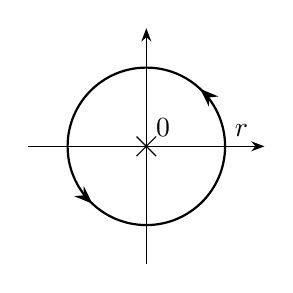
\begin{tikzpicture}
    \draw [-{Stealth}] (-1.5,0) -- (1.5,0);
    \draw [-{Stealth}] (0,-1.5) -- (0,1.5);
    \node at (1,0) [above right] {$r$};
    \node [draw=black,cross out] at (0,0) {};
    %\draw (-2pt,-2pt) -- (2pt,2pt) (2pt,-2pt) -- (-2pt,2pt);
    \node at (0,0) [above right] {$0$};
    \draw [postaction={decorate},decoration={markings,
        mark=at position .13 with {\arrow{Stealth}},
        mark=at position .63 with {\arrow{Stealth}}
    },thick]
      (1,0) arc [start angle=0, end angle=360, radius=1];
  \end{tikzpicture}
\end{wrapfigure}

積分路 $\gamma$ が半径 $r$ の円周 $\gamma(t)=re^{2\pi\ImagI t}$ の場合は,$\int_\gamma f(z)dz$ のことを
\[\int_{\abs{z}=r} f(z)dz\]
と書くことも多いです.向きは,特に断らない限り反時計回り(「正の向き」)に取ります.


\begin{example} \label{example:integrate-z^k}
  整数 $k$ について,$f(z)=z^k$ を原点の周りで(反時計回りに)一周するように積分してみます.
  %積分路は $\gamma(t)=e^{2\pi i t}$ とおきます.
  \[
  \int_{\abs{z}=r} z^k dz=\begin{cases}
  0 & k\ne -1 \\
  2\pi i & k=-1
  \end{cases}
  \]
  この積分値は積分路の半径 $r$ によらないこと,$k=-1$ の場合を覗くと積分値は $0$ となることがわかります.
\end{example}

\Section{コーシーの定理}
正則関数の積分について,次の重要な定理が成り立ちます.

\begin{theorem}[Cauchy]
  $f$ が $\Complex$ の単連結領域 $D$ で正則ならば,$D$ 内の区分的に滑らかな閉曲線 $\gamma$ について
  \[\int_\gamma f(z)dz=0.\]
\end{theorem}

「単連結」って何だよ!と思った人のために一言補足しておくと,単連結というのは内部に穴などが空いてない,ぐらいの意味です.
例えば,複素平面は単連結ですが,複素平面からいくつかの点を取り除くと単連結ではなくなります.
%複素平面から1点を取り除いた領域 $\Complex\setminus\{0\}$ で定義された関数 $f(z)=\frac{1}{z}$ についてコーシーの定理が成り立たないのは,\autoref{example:integrate-z^k} の通りです.
%複素平面や円板は単連結ですが,そこからいくつか点を取り除くと単連結ではなくなります.

この定理を使うと,例えば,複素平面全体で正則な関数は,始点と終点を決めてやればあとは積分路によらず積分値が定まることがわかります.
また,ある領域上での正則関数なら,その領域を逸脱しない範囲で積分路を多少変形させてもよいことがわかります(下図の領域内で正則な関数なら,積分路を $\gamma$ としても $\gamma'$ としても積分の値は同じ).

\begin{center}
\pgfdeclarepatternformonly{custom north east lines}{\pgfqpoint{-1pt}{-1pt}}{\pgfqpoint{8pt}{8pt}}{\pgfqpoint{7pt}{7pt}}%
{
  \pgfsetlinewidth{0.2pt}
  \pgfpathmoveto{\pgfqpoint{0pt}{0pt}}
  \pgfpathlineto{\pgfqpoint{7.1pt}{7.1pt}}
  \pgfusepath{stroke}
}
  \begin{tikzpicture}
    \draw [-{Stealth}] (-2,0) -- (2,0);
    \draw [-{Stealth}] (0,-1.8) -- (0,2);
    \draw [fill,pattern=custom north east lines] plot [smooth cycle, tension=1] coordinates {(-1.5,-0.9) (-0.3,-1) (1,-1.2) (1.6,0.3) (1.2,1.3) (0.1,1.1) (-1.1,1.2) (-1.5,0.3) (-1.5,-0.2)};
    \fill (-1,0) circle (2pt) node [above] {始点};
    \fill (1,0.2) circle (2pt) node [below=3pt] {終点};
    \draw [postaction={decorate},decoration={markings,mark=at position .58 with {\arrow{Stealth}}},thick]
      (-1,0) .. controls (0,-0.7) and (0.1,1.2) .. (1,0.2)
      node [midway,above left] {$\gamma$}
      ;
    \draw [postaction={decorate},decoration={markings,mark=at position .58 with {\arrow{Stealth}}},thick]
      (-1,0) .. controls (-0.4,-1.4) and (0.3,0.5) .. (1,0.2)
      node [midway,below right] {$\gamma'$}
      ;
  \end{tikzpicture}
\end{center}

\Section{留数}
関数 $f$ が $z=z_0$ を除いた領域で正則な時, $f$ は
%点 $z=z_0$ の除外近傍で正則な関数 $f$ を
\[f(z)=\dots+\frac{a_{-2}}{(z-z_0)^2}+\frac{a_{-1}}{z-z_0}+a_0+a_1(z-z_0)+a_2(z-z_0)^2+\dotsb\]
と展開できます.これを $f$ の $z=z_0$ におけるローラン(Laurent)展開と呼びます.

この $f$ を $z=z_0$ の周りで積分すると,\autoref{example:integrate-z^k} の結果より,
\begin{align*}
\int_{\abs{z-z_0}=r} f(z)dz
&=\int_{\abs{z-z_0}=r} \sum_{k=-\infty}^\infty a_k (z-z_0)^k dz \\
&=\int_{\abs{z-z_0}=r} \frac{a_k}{z-z_0} dz \\
&=2\pi i a_{-1}
\end{align*}
という風に,ローラン展開の $-1$ 次の係数(だけ)が出てきます.
この係数 $a_{-1}$ のことを, $f$ の $z_0$ での\ruby{留数}{りゅうすう}(residue)と呼びます.
正則関数を閉路に沿って積分する時,積分路の内部の特異点における留数が全部わかってしまえば,積分の値が決まってしまいます.

\begin{example}
  $f(z)=\frac{1}{z^3-1}$
  を考えます.
  この関数は,複素平面の $z=1,e^{2\pi i/3},e^{4\pi i/3}$ を除いた部分で定義された正則関数です.

  $f$ の $z=1$ におけるローラン展開は
  \[
  f(z)
  %=\frac{1}{(z-1)(z^2+z+1)}
  =\frac{1}{3}\frac{1}{z-1}+a_0+a_1(z-1)+\dotsb, %-\frac{1}{3}+\frac{2}{9}(z-1)+\dotsb,
  \]
  $z=e^{2\pi i/3}$ におけるローラン展開は
  \[
  f(z)
  =\frac{e^{2\pi i/3}}{3}\frac{1}{z-e^{2\pi i/3}}+a'_0+a'_1(z-e^{2\pi i/3})+\dotsb, %\frac{\sqrt{3}i}{9}+\dotsb,
  \]
  $z=e^{4\pi i/3}$ におけるローラン展開は
  \[
  f(z)
  =\frac{e^{4\pi i/3}}{3}\frac{1}{z-e^{4\pi i/3}}+a''_0+a''_1(z-e^{4\pi i/3})+\dotsb,
  \]
  となるので,それぞれの点における留数は $\frac{1}{3}$, $\frac{e^{2\pi i/3}}{3}$, $\frac{e^{4\pi i/3}}{3}$ です.

  この $f(z)$ を円周 $\abs{z}=2$ に沿って積分しましょう.
  この積分路の内部には3つの特異点が含まれます.
  \begin{center}
    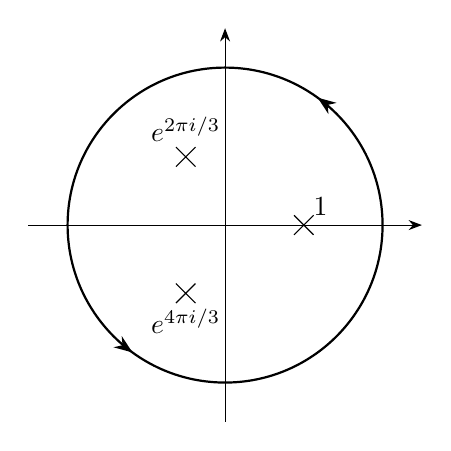
\begin{tikzpicture}
      \draw [-{Stealth}] (-2.5,0) -- (2.5,0);
      \draw [-{Stealth}] (0,-2.5) -- (0,2.5);
      \node [draw=black,cross out] at (1,0) {};
      \node [above right] at (1,0) {$1$};
      \node [draw=black,cross out] at (120:1) {};
      \node [above=2pt] at (120:1) {$e^{2\pi i/3}$};
      \node [draw=black,cross out] at (240:1) {};
      \node [below=2pt] at (240:1) {$e^{4\pi i/3}$};
      \draw [postaction={decorate},decoration={
          markings,
          mark=at position .15 with {\arrow{Stealth}},
          mark=at position .65 with {\arrow{Stealth}}
        },thick]
        (0,0) circle (2);
    \end{tikzpicture}
  \end{center}
  よって,この関数の $\abs{z}=2$ 上での積分は,内部の留数の和に $2\pi i$ をかけて,
  \[\int_{\abs{z}=2} f(z)dz=2\pi i\left(\frac{1}{3}+\frac{e^{2\pi i/3}}{3}+\frac{e^{4\pi i/3}}{3}\right)=0\]
  となります.
\end{example}


\Section{正則でない関数の例}

今までは「正則関数」,つまり複素数での意味の微分ができる関数を考えてきましたが,実数の意味での微分ができても複素数の意味での微分ができない関数というのも考えられます.
このような関数ではコーシーの定理は成り立たないので,複素積分をすると積分路の選び方によって積分の値が変わってしまいます.

\begin{example} \label{example:conjugate-integral}
  複素数にその共役を対応させる関数 $f(z)=\bar{z}$ を考えます.
  いくつかの積分路について,点 $0$ から点 $a+ib$ へ積分してみましょう.

  \begin{center}
    \begin{tikzpicture}[x=1.4cm,y=1.4cm]
      \draw [-{Stealth}] (-0.7,0) -- (2,0);
      \draw [-{Stealth}] (0,-0.7) -- (0,1.5);
      \fill (0,0) circle (2pt) node [above left] {$0$};
      \fill (1.3,1) circle (2pt) node [above right] {$a+ib$};
      \begin{scope}[thick]
        \draw [postaction={decorate},
               decoration={markings,mark=at position .5 with {\arrow{Stealth}}}
              ]
          (0,0) -- (1.3,1)
          node [midway,above left] {壱};
        \draw [
          postaction={decorate},
          decoration={
            markings,
            mark=at position .3 with {\arrow{Stealth}},
            mark=at position .8 with {\arrow{Stealth}}
          }
        ]
          (0,0) -- (1.3,0) -- (1.3,1)
          node [midway,right] {弐};
        \draw [
          postaction={decorate},
          decoration={
            markings,
            mark=at position .3 with {\arrow{Stealth}},
            mark=at position .8 with {\arrow{Stealth}}
          }
        ]
          (0,0) -- (0,1) -- (1.3,1)
          node [midway,above] {参};
      \end{scope}
    \end{tikzpicture}
  \end{center}

  なお,積分路が途中で折れ曲がっている場合は,積分路を適当に分割して足し合わせます.
  ここの例だと,弐と参はそれぞれ2つの線分に分割できるので,線分ごとにパラメーターをとって計算します.

  壱:
  $\gamma(t)=(a+ib)t$
  \[
  \int_\gamma f(z)dz
  =\int_0^1 (a-ib)t\cdot(a+ib)dt
  =\frac{a^2+b^2}{2}
  \]

  弐:
  $\gamma_1(t)=at$, $\gamma_2(t)=a+ibt$
  \begin{align*}
  \int_{\gamma_1+\gamma_2} f(z)dz
  &=\int_{\gamma_1} f(z)dz+\int_{\gamma_1} f(z)dz \\
  &=\int_0^1 at\cdot a dt+\int_0^1 (a-ibt)\cdot ib dt \\
  &=\frac{a^2}{2}+iab+\frac{b^2}{2}
  \end{align*}

  参:
  $\gamma_1(t)=ibt$, $\gamma_2(t)=at+ib$
  \begin{align*}
  \int_{\gamma_1+\gamma_2} f(z)dz
  &=\int_{\gamma_1} f(z)dz+\int_{\gamma_1} f(z)dz \\
  &=\int_0^1 (-ibt)\cdot ib dt+\int_0^1 (at-ib)\cdot a dt \\
  &=\frac{b^2}{2}+\frac{a^2}{2}-iab
  \end{align*}

  このように,3つの積分路で積分したものがどれも積分の値が異なっています.
\end{example}

\begin{exercise}
  \autoref{example:conjugate-integral} と同じ $f(z)=\bar{z}$ を,以下の閉じた積分路でそれぞれ積分せよ.

  \begin{enumerate}
  \item 長方形.
    \begin{center}
      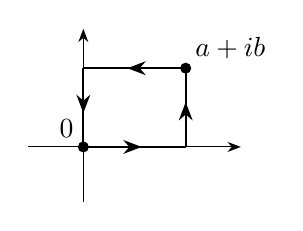
\begin{tikzpicture}
        \draw [-{Stealth}] (-0.7,0) -- (2,0);
        \draw [-{Stealth}] (0,-0.7) -- (0,1.5);
        \fill (0,0) circle (2pt) node [above left] {$0$};
        \fill (1.3,1) circle (2pt) node [above right] {$a+ib$};
        \begin{scope}[thick,
            decoration={markings,mark=at position .57 with {\arrow{Stealth}}},
            postaction={decorate}
          ]
          \draw [postaction={decorate}] (0,0) -- (1.3,0);
          \draw [postaction={decorate}] (1.3,0) -- (1.3,1);
          \draw [postaction={decorate}] (1.3,1) -- (0,1);
          \draw [postaction={decorate}] (0,1) -- (0,0);
        \end{scope}
      \end{tikzpicture}
    \end{center}

  \item 半径 $r$ の円.
  \end{enumerate}
\end{exercise}

\section*{おまけ}

今回は「たのしい複素積分」というWebページの紹介および複素積分のさわりを紹介しましたが,以前の駒場祭・五月祭では「複素関数で遊ぼう」というWebアプリの紹介をやりました.
内容は以下のURLから参照できます.
または,運の良い方なら「複素関数で遊ぼう」でググって見つけられるかもしれません.

\begin{center}
  \url{http://d-poppo.nazo.cc/math/complex-functions/}
\end{center}


\begin{thebibliography}{9}
\bibitem{Ahlfors}
  L.V. Ahlfors, \emph{Complex Analysis}, McGraw-Hill, 初版 1953, 第3版 1979.
\bibitem{Ahlfors-ja}
  L.V. アールフォルス 著 / 笠原 乾吉 訳 『複素解析』 現代数学社
\bibitem{Ueno}
  上野 健爾 『複素数の世界』はじめよう数学3, 日本評論社, 1999年
\end{thebibliography}

\end{document}

\Section{圏論が分かる4コマ漫画3(小林)}
\includegraphics[width=11cm]{kobaken3.png}
\includegraphics[width=11cm]{kobaken4.png}

{\satomacro\Chapter{線形代数の広がり(佐藤)}
線形代数という分野は古いようで新しい.そもそも「線形代数(Linear Algebra)」という言葉が現代の意味で使われ始めたのは1930年に出版されたvan der Waerdenによる「現代代数学」という教科書の中でである.しかし線形代数における重要な概念はその教科書が出版されるずっと以前から少しずつ発明されていた.例えば,未知数の数と方程式の数が一致する場合の連立一次方程式の解法(Gaussの消去法)は、中国では「漢」の時代にはすでに発見されていたし,行列式にあたる概念はLeibnizや日本では関孝和\footnote{現在でいうところの終結式の概念を導入するために行列式を発見していたというのには驚きを隠せない.}が見つけていた.その後Sylvesterにより行列の概念が導入され,Cayley,Grassmann,Jordanなど19世紀に特に行列の理論についての研究が進んだ.私たちが現在大学初年級で習っている線形代数はそれらの結果を現代的に整備したものであり,抽象度が高く応用も広い反面,なぜそういったことを考えるのかというモチベーションがわかりにくくなっているように思う.この記事では,前半で行列や行列式の概念が多変数の微積分においてどのように出てくるのかを見た後,後半で抽象的な線形空間の例として多様体の接ベクトル空間というものを導入し,一つの応用として多様体上のベクトル場を挙げることにする.

\Section{多変数の微積分}
\Subsection{多変数における微分とは何か}
微分可能な1変数関数$f:\realnum\rightarrow\realnum$の$x=a$における「微分」(正確には微分係数)は$f'(a)$で与えられるのであった.このとき,Taylorの定理より,
$$
f(x)=f(a)+f'(a)(x-a)+o((x-a))
$$
が\footnote{以下,$o(x)$は$\lim_{x\rightarrow 0}\frac{o(x)}{x}=0$を満たすような項を表しているとする.}成り立つ.特に右辺の第2項は$f$の「1次近似」を与えていると考えることができ,$x=a$における$y=f(x)$のグラフをの接線の式は$y=f'(a)(x-a)+f(a)$となる.このように微分を関数の「1次近似」を与えるものとして考え,多変数に拡張してみる.


$n$変数の$C^1$級\footnote{各成分の偏導関数$\delxkf$が連続であること.}実数値関数$f:\realnum^n\rightarrow\realnum$と$\avec\in\realnum^n$が与えられているとする.多変数のTaylorの定理から
$$
f\xvec=f\avec+\sum_{k=1}^{n}\delxkf\avec(x_k-a_k)+o\bigl(\sqrt{(x_1-a_1)^2+\cdots+(x_n-a_n)^2}\bigr)
$$
と$f$は表せる.1変数のときと同様に右辺の第2項に注目してみる.この部分は,$x={}^t\!(x_1,\dots,x_n), a={}^t\!(a_1,\dots,a_n), J=\left(\delxof(a_1,\dots,a_n) \dots \delxnf(a_1,\dots,a_n)\right)$とおくと\footnote{紙面の節約のため縦ベクトル$\vecb x_1 \\ \vdots \\ x_n\vece$を${}^t\!(x_1,\dots,x_n)$と書く.}行列とベクトルの積$J(x-a)$と書けるから,上の式は
$$
f(x)=f(a)+J(x-a)+o(|x-a|)
$$
という非常にすっきりした形で表せる.特に,$x=a$における「接平面」の式は$y=J(x-a)+f(a)$となる.
さて,幾何学的に見れば,$\delxkf(a_1,\dots,a_n)$達はそれぞれ$(a_1,\dots,a_n)$における$e_k=\tenchi(0,\dots,1,\dots,0)$($k$番目の成分は1,それ以外は0)方向の変化率を表しているのだが,では一般に単位ベクトル$b=\tenchi(b_1,\dots,b_n)$方向の変化率はどう表せるだろうか.勿論極限の式から直接導くことは出来るが、ここでは接平面が$y=J(x-a)+f(a)$であることに注目すると,接平面における$b$方向の傾きは$Jb=\dsum_{k=1}^{n}\delxkf(a_1,\dots,a_n)b_k$であることから,$b$方向の$f$の変化率が$Jb$であることが簡単にわかる(もし$b$が単位ベクトルでない場合は$\dfrac{Jb}{|b|}$とあらわせる).このことから,$J$は$f$の$a$における全ての方向における1次近似の情報を持っていると見なせる.この$J$を上にならって$f$の$a$における「微分」と呼ぶことにしよう.


今までの議論は$f$の値域が$\realnum$,すなわち1次元の場合であった.もっと一般に$C^1$級写像$f:\realnum^n\rightarrow\realnum^m$が与えられたとする.結局値域が広がったところで,$m$個の$C^1$級関数$f_1,\dots,f_m$によって,$f\xvec=(f_1\xvec,\dots,f_m\xvec)$とあらわされるので,各$f_i:\realnum^n\rightarrow\realnum$について,1行$n$列の行列$J_i$が存在して,1次近似は$f_i(x)=f_i(a)+J_i(x-a)+o(|x-a|)$となる.この式を縦に並べて,$J=\vecb J_1\\ \vdots \\J_m\vece$という$m$行$n$列の行列を考えると,$f(x)=\tenchi(f_1(x),\dots,f_m(x)),f(a)=\tenchi(f_1(a),\dots,f_m(a))$と縦ベクトルで表せば,
$$
f(x)=f(a)+J(x-a)+o(|x-a|)
$$
という上と全く同じ式が得られる(ただし,この式は$m$次元ベクトルの等式なので,$o(|x-a|)$は各成分が$o(|x-a|)$であるようなベクトルを表していることに注意).上の式は特に$b\in\realnum^n$が十分小さいとき,$f(a+b)-f(a)\approx J(b)$と書けることを示していて,$f$によって$a$の$n$次元空間における「方向」が$f(a)$の$m$次元空間におけるどの「方向」に移るかを$J$は表していると考えられる.こうして多次元での微分を考える際には自然と行列の概念が出てくる.


$J$倍写像$\realnum^n\rightarrow\realnum^m$を「$n$次元方向」を「$m$次元方向」へ移す写像と考えたとき,$J$は次の性質をもつ.
\begin{enumerate}
\renewcommand{\labelenumi}{(\theenumi)}
\item 任意の$\lambda\in\realnum, x\in\realnum^n$に対して,$J(\lambda x)=\lambda J(x)$
\item 任意の$x,y\in\realnum^n$に対して,$J(x+y)=J(x)+J(y)$
\end{enumerate}
この性質によって,任意の$b=\tenchi(b_1,\dots,b_n)$に対して,$Jb=J(b_1e_1+\dots+ b_ne_n)=b_1J(e_1)+\dots+b_nJ(e_n)$となるが,$J$を成分によって明示的に表すと,
$$
J=\vecb \delxofo && \dots && \delxnfo \\ \vdots && && \vdots \\ \delxofm && \dots&&\delxnfm \\ \vece
$$
であるので,$J(e_k)=\tenchi\left(\delxkfo,\dots,\delxkfm\right)$となる.特に,$J$の各列ベクトルの線形結合によって,$Jb$は表される.すなわち,値域が$\realnum$から$\realnum^m$になっても$J$がすべての方向に関する1次近似の情報を持っていることには変わりがない.ところで,上の性質を満たすような$\realnum^n$から$\realnum^m$への写像は,ある行列$A$を用いて$A$倍写像とあらわされることが知られている.上の性質を満たすような写像を$\realnum^n$から$\realnum^m$への線形写像という.


まとめると,微分は$f:\realnum^n\rightarrow\realnum^m$の$a\in\realnum^n$における線形写像による近似を与えることと考えることが出来る.
このとき,この線形写像に対応する行列$J_f$をヤコビ行列という.ヤコビ行列の一つの応用として,微分の連鎖律を説明してみよう.
\begin{s_theo}[微分の連鎖律]
2つの$C^1$級写像$f:\realnum^n\rightarrow\realnum^m$と$g:\realnum^m\rightarrow\realnum^l$が与えられたとする.
このとき$J_{g\circ f}$で$a\in\realnum^n$における$g\circ f$のヤコビ行列
$J_f,J_g$で$f,g$の$a,f(a)$におけるヤコビ行列を表すと,
\[
J_{g\circ f}=J_gJ_f
\]
が成り立つ.
\end{s_theo}
\begin{Proof}
まず,$f,g$の1次近似は$f(a+b)-f(a)=J_f(b)+o(b),g(f(a)+b')-g(f(a))=J_g(b')+o(b')$と書けるから,$g(f(a+b))-g(f(a))=g(f(a)+f(a+b)-f(a))-g(f(a))=g(f(a)+J_f(b)+o(b))-g(f(a))=J_g(J_f(b)+o(b))+o(J_f(b)+o(b))=J_g(J_f(b))+o(b)$となる(最後の等号は,線形写像の性質(2)より$J_g(J_f(b)+o(b))=J_g(J_f(b))+J_g(o(b))$および,性質(1)と連続性より任意の線形写像$f$について,$f(o(x))=o(x),o(f(x))=o(x)$が成り立つことによる).よって,$g\circ f$の1次近似は$J_g$倍写像と$J_f$倍写像の合成で表される.ところで,行列の積の結合法則より,任意の$x\in\realnum^n$に対して$J_g(J_fx)=(J_gJ_f)x$が成り立つから,$J_g$倍写像と$J_f$倍写像の合成は$J_gJ_f$倍写像である.よって$J_{g\circ f}=J_gJ_f$となる.これが連鎖律とどう関係するかというと,両辺の成分を比べてみると,$\realnum^n$の変数を$x_1,\dots,x_n$,$\realnum^m$の変数を$y_1,\dots,y_m$として

$$
\vecb
\dfrac{\partial (g\circ f)_1}{\partial x_1}(a) && \dots && \dfrac{\partial (g\circ f)_1}{\partial x_n}(a) \\
\vdots                                           &&         && \vdots \\
\dfrac{\partial (g\circ f)_l}{\partial x_1}(a)  && \dots && \dfrac{\partial (g\circ f)_l}{\partial x_n}(a) \\
\vece
=
\vecb
\dfrac{\partial g_1}{\partial y_1}(f(a)) && \dots && \dfrac{\partial g_1}{\partial y_m}(f(a)) \\
\vdots                                           &&         && \vdots \\
\dfrac{\partial g_l}{\partial y_1}(f(a))  && \dots && \dfrac{\partial g_l}{\partial y_m}(f(a)) \\
\vece
\vecb
\dfrac{\partial f_1}{\partial x_1}(a) && \dots && \dfrac{\partial f_1}{\partial x_n}(a) \\
\vdots                                           &&         && \vdots \\
\dfrac{\partial f_m}{\partial x_1}(a)  && \dots && \dfrac{\partial f_m}{\partial x_n}(a) \\
\vece
$$
両辺の成分を比較して,$\dfrac{\partial (g\circ f)_i}{\partial x_j}(a)=\dsum_{k=1}^m\dfrac{\partial g_i}{\partial y_k}(f(a))\dfrac{\partial f_k}{\partial x_j}(a)$という等式を得る.
\end{Proof}

\Subsection{ヤコビ行列の応用と行列式}
前節においてヤコビ行列というものを導入したわけだが,ヤコビ行列は単なる1次近似の情報だけでなく,実は色々な情報を持っている.その例として逆関数定理と重積分の変数変換公式を紹介しよう.
\Subsubsection{逆関数定理}
まず,ヤコビ行列の行列式が$0$でないことはどういう情報であるかを表す\textbf{逆関数定理}について紹介する.
そのために,「開集合」という概念について説明しておく.「$\realnum^n$の部分集合$U$が$\realnum^n$の開集合である」とは,$U$の各点$x$に対して,十分小さい$\varepsilon>0$を取れば$x$から距離$\varepsilon$以内の点がすべて$U$に入るような集合のことを言う.直観的に言えば,開集合とは外部と接しているような点がないような集合のことで,例えば$\{(x,y)\in\realnum^2\mid x^2+y^2<1\}$は$\realnum^2$の開集合だが,$\{(x,y)\in\realnum^2\mid x^2+y^2\le1\}$はそうでない.$x\in\realnum^2$が入っているような$\realnum^n$の開集合のことを「$x$の$\realnum^n$における開近傍」という.ここで,$a\in\realnum^n$で微分するという操作は,$a$の十分近くで$f$が定義されていれば行えることに注意しよう(簡単な例として,$f(x)=\frac{1}{x}$は0以外のどこでも微分できるのであった).すると微分しようとする写像$f$は必ずしも$\realnum^n$全体で定義されている必要はなく,$a$の開近傍上で定義されていれば十分ということがわかる.準備が出来たところで逆関数定理のステートメントを述べよう.
\begin{s_theo}[逆関数定理]
$W$を$a\in\realnum^n$の$\realnum^n$における開近傍,$f:W\rightarrow\realnum^n$を$C^1$級写像とする.$a$における$f$のヤコビ行列$J_f$について,$J_f$の行列式$\det(J_f)$が0でないとき,$W$に含まれる$a$の$\realnum^n$におけるある開近傍$U$,$f(U)\subset V$をみたす$f(a)$の$\realnum^n$におけるある開近傍$V$,および$C^1$級写像$g:V\rightarrow U$が存在して,$f$の$U,V$への制限$\tilde{f}:U\rightarrow V$と$g$は互いに逆写像
\footnote{写像$p:A\rightarrow B$と$q:B\rightarrow A$が互いに逆写像とは,任意の$a\in A$に対して,$q(p(a))=a$および任意の$b\in B$に対して$p(q(b))=b$が成り立つことを言うのであった.}になっている.
\end{s_theo}
この定理は,\textbf{写像$f$の$a$におけるヤコビアンが$\det(J_f)$が$0$でなければ,$a$の周りで「局所的に」$f$はなめらかな逆写像を持つ,}ということを言っている.具体的に見てみよう.
\begin{figure}[h]
  \begin{center} 
    \includegraphics[width=7.0cm]{dev_invfunc}
    \caption{逆関数定理のイメージ}
  \end{center}
\end{figure}
\begin{s_ex}
$f:\realnum^2\rightarrow\realnum^2;(x,y)\mapsto(x+y,xy)$という写像を考えてみる.$f$は単射でも全射でもない.たとえば$f(2,1)=(3,2)=f(1,2)$であるし,$f(x,y)=(1,3)$を満たす$x,y\in\realnum$は存在しない.よって逆写像は存在しない.ここで,$(2,1)\in\realnum$においてヤコビ行列を計算してみると,
$$
\det(J_f)=\detb 1 && 1 \\ 1&& 2 \dete = 1\neq 0
$$
より,逆関数定理から,$(2,1)$の開近傍で逆写像をもつ.実際,$U=\{(x,y)\in\realnum^2\mid x>y\},V=\{(s,t)\in\realnum^2\mid s^2-4t>0\}$とおくと,$U$は$(2,1)$の$\realnum^2$における開近傍,$V$は$(3,2)$の$\realnum^2$における開近傍で$f(U)\subset V$であり,$C^1$級写像$g:V\rightarrow U$を$(s,t)\mapsto\left(\frac{s+\sqrt{s^2-4t}}{2},\frac{s-\sqrt{s^2-4t}}{2}\right)$と定めると,$f$の制限$\tilde{f}:U\rightarrow V$と$g$は互いに逆写像となっている.
\end{s_ex}
この定理では$\det(J_f)\neq 0$という条件が一番本質的である.行列式の定義を思い出してみよう.$n$個の$\realnum^n$のベクトル$p_1,\dots,p_n$が与えられたとき,$P=(p_1\: p_2\dots p_n)$の行列式が0という条件は,$p_1,\dots,p_n$が一次従属であることと同値だった.直観的に言えば,$p_1,\dots,p_n$で張られる$n$次元平行四辺形の体積が潰れていなければ,$\det(P)\neq 0$となる.これを使って定理の直観的な説明を与えよう.$f$が仮定を満たすとする.$J_f$は$a$における線形近似を表していたので,$\lambda>0$が十分0に近ければ,$A=\{a+(x_1e_1+\dots+x_ne_n)\in\realnum^n\mid 各kについて|x_k|<\lambda\}$という$a$を含む微小長方形内では,$f$は$J_f$が表す線形写像で近似でき,その像は$B=\{f(a)+(x_1J_f(e_1)+\dots +x_nJ_f(e_n))\mid 各kについて|x_k|<\lambda\}$という,$J_f$の列ベクトルが張る微小平行四辺形に(だいたい)移ると考えられる.今$J_f$の列ベクトルは1次独立だから,$B$は$\realnum^n$内の開集合であり,$\det(J_f)\neq 0$より$J_f$には逆行列が存在するから,$J_f$の逆行列が表す線形写像$g:B\rightarrow A$を考えれば,$f:A\rightarrow B$と$g:B\rightarrow A$は(だいたい)逆写像になっている.ここでいちいち(だいたい)と付けたのは,実際に証明する段階ではこの説明どおりに話は進まないからだが,実際に使用する際のイメージとしてはこれくらいの認識でも十分だと思う.

\Subsubsection{重積分の変数変換公式}
ヤコビ行列の行列式をヤコビアンという.ところで,上の定理ではヤコビアンが0かどうかという情報しか使われていなかったが,ヤコビアンの値そのものが使われるような場面はあるのだろうか.それが次の重積分の変数変換公式である.
\begin{s_theo}[変数変換公式]
$D,D'$を積分可能な$\realnum^n$のコンパクト集合\footnote{原点から一定の距離に収まるような集合であって,補集合が開集合となるようなもの.}とする.$C^1$級写像$g:D\rightarrow D'$が全単射であり,任意の$x\in D$に対して,$x$での$g$のヤコビアン$\det(J_g(x))$\footnote{ここだけ$J_g(x)$と書いてしまったが,これは線形写像$J_g$の$x$における値ではなく,$x$におけるヤコビ行列のことである.}が0でないとする.このとき,$D'$上の連続値関数$f$について,
$$
\int_{D'}f(y)dy=\int_Df(g(x))|\det(J_g(x))|dx
$$
が成り立つ.
\end{s_theo}
細かい条件はさておき,これも大体上で説明したようなイメージで説明できる.任意の$x\in D$の周りにおいて,$A=\{x+(x_1e_1+\dots+x_ne_n)\in\realnum^n\mid 各kについて|x_k|<\lambda\}$という微小長方形は,$g$によって$B=\{g(x)+(x_1J_g(e_1)+\dots +x_nJ_g(e_n))\mid 各kについて|x_k|<\lambda\}$という,$J_g$の列ベクトルが張る微小平行四辺形に(だいたい)移る.このとき,$B$の体積は$A$の体積の$\lvert\det(J_g)\rvert$倍になっているので,微小体積を比べると$dy=\lvert\det(J_g)\rvert dx$になっているため,上のような積分の式が成り立つ.ここで,わざわざ行列式に絶対値がついているのは,$\realnum^n$を「ひっくり返す」ような線形写像(例えば$\realnum^2$なら$(x,y)\mapsto (y,x)$など)に対しては,行列式の値が負になってしまい,積分の符号が反転するのを防ぐためである.


さて,上の定理は若干強い形で書いたが,実は$D$において$\det(J_g)$が0になるようなところが多少あっても,上の式は成り立つ.詳しく言えば,ある体積0の部分集合$N\subset D$があって,ヤコビアンが0になる点がすべて入っており,$g$は$D-N$から$D'$への全単射になっていれば上の式が成り立つ.最後に具体例として,$\realnum^3$における直交座標から極座標への変数変換を考えてみよう.今,$D=\{(r,\theta,\varphi)\in\realnum^3\mid 0\le r\le1,0\le \theta \le \pi,0\le \varphi \le 2\pi\},D'=\{(x,y,z)\in\realnum^3\mid x^2+y^2+z^2\le 1\},$とおき,$g:D\rightarrow D'$を$(r,\theta,\varphi)\mapsto (r\sin\theta\cos\varphi,r\sin\theta\sin\varphi,r\cos\theta)$とすると,$g$は仮定の条件を満たしていることがわかる.$\det(J_g)$は(やや煩雑な計算をすると)$r^2\sin\theta$となる.よって,例えば$f=1$(恒等写像)とすると,
$$
\int_{D'}dxdydz=\int_{D}r^2\sin\theta\,dr d\theta d\varphi=\frac{4}{3}\pi
$$
となって,単位球の体積がわかる.同様の方法で$n$次元単位球の体積が$\sin^m\theta\quad(1\le m\le n-2)$達の積分と$\frac{1}{n}$の積に帰着され,$\Gamma$関数を使って$\dfrac{\pi^{\frac{n}{2}}}{\Gamma(\frac{n}{2}+1)}$とあらわせる.(興味がある人は計算してみよう.)


\Section{幾何学へ}
\Subsection{線形空間と接ベクトル空間}
前の章では写像$f:\realnum^n\rightarrow\realnum^m$の微分を考えたが,もっと一般の写像について微分の概念を考えてみたい.そこで,「球面$S^2=\{(x,y,z)\in\realnum^3\mid x^2+y^2+z^2=1\}$に対して,$S^2$上の関数$f:S^2\rightarrow\realnum$の微分とは何だろうか」という問題を考えてみる.球面上の関数とは何ぞや?と思われるかもしれないが,例えば地球上の温度やら人口密度やらを考えてもらえば十分である.


$S^2$が存在する空間は3次元であるが,$S^2$そのものは2次元と捉えたい.それは,世界地図が2次元の紙に印刷されていることからも推察できる.しかし,$S^2$から$\realnum^2$の開集合への同相写像\footnote{連続写像であって,逆写像も連続な写像のこと.まだ一般の$\realnum^3$の部分集合$A$上の連続写像というものを定義していないが,今は次のように定義しておこう.$A,B$をそれぞれ$\realnum^n,\realnum^m$の部分集合とする.$f:A\rightarrow B$が連続とは,$A$を含むような$\realnum^n$のある開集合$U$と連続写像$F:U\rightarrow \realnum^m$が存在して,任意の$x\in A$に対して$f(x)=F(x)$を満たすこととする.}は実は存在しない.しかし,$S^2$の開集合$U$に対しては\footnote{$\realnum^n$の部分集合$A$について,$U$が$A$の開集合であるとは,ある$\realnum^n$の開集合$U'$が存在して,$U=A\cap U'$となることとする.},$\realnum^2$の部分集合との同相写像は存在する.たとえば,$V_{x+}=\{(y,z)\in \realnum^2\mid y^2+z^2<1\}$という$\realnum^2$の開集合から,$U_{x+}=\{(x,y,z)\in S^2\mid x>0\}$という$S^2$の開集合への連続写像$\varphi_{x+}:V_{x+}\rightarrow U_{x+}$を$(y,z)\mapsto (\sqrt{1-y^2-z^2},y,z)$で定めると,$\varphi_{x+}$は$\varphi_{x+}^{-1}:U_{x+}\rightarrow V_{x+};(x,y,z)\mapsto (y,z)$という逆写像を持ち,逆写像も連続であるので,同相写像となっている.他に,$U_{y+}=\{(x,y,z)\in S^2\mid y>0\},V_{y+}=\{(x,z)\in\realnum^2\mid x^2+z^2<1\}$に対しては,$\varphi_{y+}:V_{y+}\rightarrow U_{y+};(x,z)\mapsto (x,\sqrt{1-x^2-z^2},z)$,あるいは,$U_{z-}=\{(x,y,z)\in S^2\mid z<0\},V_{z-}=\{(x,y)\in\realnum^2\mid x^2+y^2<1\}$に対しては,$\varphi_{z-}:V_{z-}\rightarrow U_{z-};(x,y)\mapsto (x,y,-\sqrt{1-x^2-y^2})$などなど,他も同様に定めれば合計$6$つの開集合$U_{x\pm},U_{y\pm},U_{z\pm}$によって,$S^2$は覆われる.このような$U$と$\varphi$の組$(\varphi;U)$を$S^2$の「局所座標」と呼ぶことにしよう.


さて,前章で微分は写像に対して線形写像を対応させる操作であることを見たのだが,そもそもこの場合,どこからどこへの線形写像を考えればいいのだろうか.「方向」を「方向」に移すというおおもとの考えに戻ってみると,球面上の「方向」を$\realnum$の「方向」に移す線形写像を考えればいいことがわかる.$\realnum$の方向は前章と同じく$\realnum$とすると,問題なのは$S^2$上の「方向」である.具体的に$p=\left(\frac{1}{\sqrt{3}},\frac{1}{\sqrt{3}},\frac{1}{\sqrt{3}}\right)$における$f$の微分を考えてみよう.今例えば$S^2$を,$(0,0,1)$を北極とする地球だとみなして,$p$における$f$の東の経線方向の微分を考えよう.$p$を通るような東向きの経線は$\gamma:\realnum\rightarrow S^2;t\mapsto\left(\sqrt{\frac{2}{3}}\cos(t+\frac{\pi}{4}),\sqrt{\frac{2}{3}}\sin(t+\frac{\pi}{4}),\frac{1}{\sqrt{3}}\right)$という曲線で与えられる.$\gamma$と$f$の合成によって,$f\circ \gamma:\realnum\rightarrow\realnum$が得られ,$t=0$で$\gamma$は$p$を通るので,$f\circ\gamma$が$t=0$で微分可能なら$\dfrac{d(f\circ\gamma(t))}{dt}\Big|_{t=0}$が$p$での$f$の東向きの経線方向の微分であることが分かる.


このことをもとに,球面上の「方向微分」の概念を考えてみる.$t=0$で$p$を通るような全ての$S^2$上の曲線$\gamma$に\footnote{以後,「曲線」と言った場合,十分なめらか,すなわち何回でも微分できるようなもののみを指す.}ついて$\gamma$方向の$f$の微分を$\dfrac{d(f\circ\gamma(t))}{dt}\Big|_{t=0}$によって定める.これは偏微分の概念の一般化になっていることに注意しよう.というのも,$f$の定義域が$\realnum^n$の開集合の場合は$\delxkf(p)=\lim_{h\rightarrow 0}\dfrac{f(p+he_k)-f(p)}{h}=\dfrac{d(f(p+te_k))}{dt}\Big|_{t=0}$と書けるから,$\gamma(t)=p+te_k$とすれば,偏微分は特別な$\gamma$に対する方向微分の値に過ぎない.しかし同時に,$f$の定義域が$\realnum^n$の開集合である場合は,従来考えていた$\realnum^n$のベクトル方向の微分を考えれば十分であるというのもわかる.というのも,曲線$\gamma:(c,d)\rightarrow \realnum^n$ (ただし,$(c,d)\subset\realnum$は0が入るような開区間を表す.)に対して$\dfrac{d\gamma}{dt}\Big|_{t=0}=(b_1,b_2,\dots,b_n)$とおくと,連鎖律から$\dfrac{d(f\circ\gamma(t))}{dt}\Big|_{t=0}=\delxof(p) b_1+\dots+\delxnf(p) b_n$と書けるから.結局これは元の意味での$(b_1,\dots,b_n)$方向の微分に他ならない.
\begin{figure}[h]
  \begin{center} 
    \includegraphics[width=7.0cm]{dev_tangentvec}
    \caption{方向微分と接ベクトル空間}
  \end{center}
\end{figure}


$\realnum^n$のときは$\delxkf(p)$達の値が分かっていれば,他の方向に関する微分はそれらの線形結合で表せたが,$S^2$のときはいちいち対応する曲線を求めなくてはいけないのだろうか.ここで,最初に考えていた,局所座標$(\varphi_{x\pm};U_{x\pm}),(\varphi_{y\pm};U_{y\pm}),(\varphi_{z\pm};U_{z\pm})$達が役に立つのである.今,$p$は$U_{x+}$に入っていることから,$\varphi_{x+}^{-1}$によって$q=(\frac{1}{\sqrt{3}},\frac{1}{\sqrt{3}})\in V_{x+}$に移る.$\gamma$を$t=0$で$p$を通る曲線とする.$\gamma$(の$U_{x+}$に入っている部分)を$\varphi_{x+}^{-1}$によって$V_{x+}$に移すと,$V_{x+}$上の曲線$\tilde{\gamma}$が得られる.このとき,$\tilde{\gamma}(0)=q$であり,$\dfrac{d\tilde{\gamma}}{dt}\Big|_{t=0}=(b_1,b_2)$とおくと,今$f\circ \varphi_{x+}$の定義域は$\realnum^2$の開集合であるから,先程の議論より$f\circ\varphi_{x+}$の$\tilde{\gamma}$方向の微分は$\dfrac{\partial (f\circ\varphi_{x+})}{\partial y}(q)b_1+\dfrac{\partial (f\circ\varphi_{x+})}{\partial z}(q)b_2$と表せる.ここで,$f\circ \varphi_{x+}$の$\tilde{\gamma}$方向の微分は$\dfrac{d(f\circ\varphi_{x+}\circ\tilde{\gamma}(t))}{dt}\Big|_{t=0}=\dfrac{d(f\circ\varphi_{x+}\circ\varphi_{x+}^{-1}\circ\gamma(t))}{dt}\Big|_{t=0}=\dfrac{d(f\circ\gamma(t))}{dt}\Big|_{t=0}$となって,$f$の$\gamma$方向の微分と等しい.よって全ての方向の微分は$\dfrac{\partial (f\circ\varphi_{x+})}{\partial y}(q),\dfrac{\partial (f\circ\varphi_{x+})}{\partial z}(q)$の線形結合で与えられることが分かる.


しかしだからといって$f\circ \varphi_{x+}$のヤコビ行列$J_{f\circ \varphi_{x+}}$について,$J_{f\circ\varphi_{x+}}$倍写像$\realnum^2\rightarrow \realnum$そのものを$f$の微分とするのはいささか抵抗がある.というのも,$p$は$U_{y+},U_{z+}$上の点でもあるので,$\varphi_{x+}$との合成だけ特別扱いするのは変だからである.しかも,一般には$J_{f\circ\varphi_{x+}}\neq J_{f\circ\varphi_{y+}}$であるから,別の局所座標を取れば別のヤコビ行列が得られる.なぜこのようなことがおきるのかというと,これらの線形写像の定義域が局所座標の取り方に依存してしまうからである.では$p$における全ての「方向」の空間を局所座標に依らない形で定義するにはどうすればいいだろうか.$p$を通るような曲線$\gamma$について,$\gamma$方向の$f$の微分が考えられたので,そのような$\gamma$全体の集合を「方向」の集合とすればよいと思うかもしれないが,そのような集合は大きすぎて,その中で和やスカラー倍をどう定義するかは自明ではない.和やスカラー倍が定義されていない集合を定義域とする写像では,そもそも「線形写像」の概念を考えられない.


ここで,発想の転換を行う.今まで思い描いてきた理想像は,適当な関数$f$が与えられると,「$p$における方向全体の集合」から$\realnum$への線形写像が一つ定まるというものだった.これは,適当な関数$f$と$p$における方向を定めると,実数が定まるということにになる.すなわち見方を変えると,$p$における方向が与えられると,「微分可能な関数」全体から$\realnum$への写像が一つ定まるということになる.この「微分可能な関数」全体から$\realnum$への写像全体の部分集合として,「$p$における方向全体の集合」を定義してしまおう.微分をまだ定義していないのに「微分可能な関数」を定めるのは変な感じを受けるかもしれないが,局所座標を用いれば簡単に定義できる.「微分可能な関数」の集合$C^\infty(S^2)$を次のように定める.$f:S^2\rightarrow \realnum$が$C^{\infty}$級であるとは,任意の$p\in S^2$に対して$p$が入るような局所座標$(\varphi;U)$を1つ取った時,$f\circ\varphi:\varphi^{-1}(U)\rightarrow \realnum$が$\varphi^{-1}(p)$で$C^{\infty}$級\footnote{つまり,任意の自然数$n,m$に対して,$\dfrac{\partial^{n+m}f}{\partial x_1^n\partial x_2^m}$が存在するということ.}であることをいい,$C^\infty$級の関数全体を$C^\infty(S^2)$で表す.


今,$C^{\infty}(S^2)$から$\realnum$への写像全体を$\mathcal F$と置くと,$\mathcal F$上には「和」と「($\realnum$による)スカラー倍」が定義される.具体的には,2つの${\mathcal F}$の元$D,D':C^{\infty}(S^2)\rightarrow \realnum$と$\lambda\in\realnum$に対して,$\lambda D,D+D'\in{\mathcal F}$を任意の$f\in C^{\infty}$に対し$(\lambda D)(f)=\lambda(D(f)),(D+D')(f)=D(f)+D'(f)$と定めればよい.このように「和」と「($\realnum$による)スカラー倍」が定義されていて,結合法則などのいくつかの良い性質を満たす集合を,「$\realnum$線形空間\footnote{$\realnum$が明らかなときはしばしば省略される.}」という.さて,$\delyp,\delzp$という$\mathcal F$の元を,
$$
\delyp:f\mapsto \dfrac{\partial (f\circ\varphi_{x+})}{\partial y}(\varphi_{x+}^{-1}(p))\quad
\delzp:f\mapsto \dfrac{\partial (f\circ\varphi_{x+})}{\partial z}(\varphi_{x+}^{-1}(p))
$$
と定め,これらの線形結合で表されるような$\mathcal F$の元,すなわちある$b_1,b_2\in\realnum$を用いて$b_1\delyp+b_2\delzp$と書けるような元全体を$T_pS^2$とおく.この集合は定義から「和」と「スカラー倍」について閉じている.すなわち,任意の$D,D'\in T_pS^2$および$\lambda\in\realnum$に対し,$\lambda D,D+D'\in T_pS^2$となる.このような線形空間の部分集合を「部分空間」という.線形空間の部分空間はそれ自身が線形空間になっている.$T_pS^2$は$S^2$における「接ベクトル空間」と呼ばれる.


いきなり天下り的に接ベクトル空間$T_pS^2$というものが導入されてしまったが,これこそが求めていた$p$における「方向」全体の集合になっている.というのも,$\gamma(0)=p$を満たす曲線$\gamma$について,$\gamma$の方向微分$D_\gamma:C^{\infty}(S^2)\rightarrow\realnum$は$D_\gamma(f)=\dfrac{d(f\circ\gamma(t))}{dt}\Big|_{t=0}$で与えられたのだったが,これは結局$\gamma$を局所座標$(\varphi_{x+};U)$によって$V_{x+}$上の曲線$\tilde{\gamma}$とみることによって,$\dfrac{d\tilde{\gamma}}{dt}\Big|_{t=0}=(b_1,b_2)$とおくと,
$$D_\gamma(f)=\dfrac{d(f\circ\varphi_{x+}\circ\tilde{\gamma}(t))}{dt}\Big|_{t=0}=\dfrac{\partial (f\circ\varphi_{x+})}{\partial y}(\varphi_{x+}^{-1}(p))b_1+\dfrac{\partial (f\circ\varphi_{x+})}{\partial z}(\varphi_{x+}^{-1}(p))b_2=\left(b_1\delyp+b_2\delzp\right)(f)
$$
となって$D_{\gamma}\in T_pS^2$がわかり,逆に,任意の$b_1,b_2\in\realnum$に対して,$b=\tenchi(b_1,b_2)$とし,$\realnum^2$の曲線$\tilde{\gamma'}:\realnum\rightarrow\realnum^2$を$\tilde{\gamma'}(t)=\varphi_{x+}^{-1}(p)+tb$で定め,$V_{x+}$に入っている部分を$\varphi_{x+}$によって$S^2$上に送った曲線を$\gamma'$と置くと,$\gamma'$の方向微分$D_{\gamma'}$は$b_1\delyp+b_2\delzp$となる.よって$p$における任意の「方向」は$T_pS^2$の元として表され,$T_pS^2$の任意の元は$p$における方向を表すので$T_pS^2$は$p$における「方向」全体の集合と見なせる.$p$における「方向」は,すなわち,$p$における$S^2$の接平面を表していると考えることもできるため,「接ベクトル空間」という名前になっているのである.



ここで一つ注意したいのが,$T_pS^2$は定義の際に局所座標$(\varphi_{x+};U_{x+})$を使っているが,実は局所座標の取り方によらない.例えば,別の局所座標$(\varphi_{y+};U_{y+})$を取ってみよう.このとき,
$$
\delxp':f\mapsto \dfrac{\partial (f\circ\varphi_{y+})}{\partial x}(\varphi_{y+}^{-1}(p))\quad
\delzp':f\mapsto \dfrac{\partial (f\circ\varphi_{y+})}{\partial z}(\varphi_{y+}^{-1}(p))
$$
という2つの$\mathcal F$の元がそれぞれ$T_pS^2$に入っていることを示せば,$\delxp',\delyp'$の線形結合で表されるような元全体$A$が$T_pS^2$に含まれていることが示せ,対称性より逆に$T_pS^2$が$A$に含まれていることが分かり,結局$T_pS^2=A$となって局所座標の取り方に依らない.今,$\varphi_{x+}^{-1}\circ\varphi_{y+}:\varphi_{y+}^{-1}(U_{x+}\cap U_{y+})\rightarrow\varphi_{x+}^{-1}(U_{x+}\cap U_{y+})$が$\realnum^2$の開集合から$\realnum^2$の開集合への写像になっていることを考えると,1章における連鎖律からら,$J_{f\circ\varphi_{y+}}=J_{f\circ\varphi_{x+}}J_{\varphi_{x+}^{-1}\circ\varphi_{y+}}$となる.ここで$J_{\varphi_{x+}^{-1}\circ\varphi_{y+}}$は$f$に依らないから,$J_{\varphi_{x+}^{-1}\circ\varphi_{y+}}=\vecb c_{11} && c_{12} \\ c_{21} && c_{22}\vece$とおくと,上の式は,
$$
\left(\delxp'(f)\quad\delzp'(f)\right)=\left(\delyp(f)\quad\delzp(f)\right)\vecb c_{11} && c_{12} \\ c_{21} && c_{22}\vece
$$
となる.任意の$f$について上の式は成り立つから,$\mathcal F$の元として
$$
\left(\delxp'\quad\delzp'\right)=\left(\delyp\quad\delzp\right)\vecb c_{11} && c_{12} \\ c_{21} && c_{22}\vece
$$
が成り立つので,各成分を比較すれば,$\delxp',\delzp'$が$T_pS^2$に入っていることが示される.


\Subsection{微分写像とrank}
さて,前節では苦労を重ねて$p$における$S^2$の方向の集合$T_pS^2$が局所座標に依らない形で定義出来たわけだが,ここまで定義されれば$f\in C^{\infty}(S^2)$の$p$における微分は簡単に定義できる.$D\in T_pS^2$の元に対して,$D(f)\in \realnum$を対応させる写像を$(df)_p:T_pS^2\rightarrow \realnum$とあらわし,$f$の$p$における微分写像という.これは定義から線形写像,すなわち任意の$\lambda\in\realnum, D,D'\in T_pS^2$に対して,$(df)_p(\lambda D)=\lambda (df_p)(D)$および$(df)_p(D+D')=(df)_p(D)+(df)_p(D')$が成り立っていることがすぐわかる.しかし,$(df)_p$は抽象的な空間から$\realnum$への線形写像なので,どのような写像なのかよくわからない.ここで,線形空間を理解するための一つのツールとして,「基底」というものを導入しよう.$T_pS^2$の元は$b_1,b_2\in\realnum$を用いて$b_1\delyp+b_2\delzp$とあらわされているのだった.もし,この表示が一意的ならば,$\realnum^2$から$T_pS^2$への写像
$(b_1,b_2)\mapsto b_1\delyp+b_2\delzp$が全単射線形写像となり,$T_pS^2$は$\realnum^2$と線形空間として「同型」,すなわちこの基底を介して,$\realnum^2$と$T_pS^2$は同じものと見なせる.さて,$b_1\delyp+b_2\delzp$という表示が一意的かどうか確かめるためには,$b_1\delyp+b_2\delzp=0$となる$b_1,b_2$が$(b_1,b_2)=(0,0)$のみ,すなわち$\delyp$と$\delzp$が1次独立であることを確かめればよい.$b_1\delyp+b_2\delzp=0$とする.これは$\mathcal F$における等式だから,すなわち任意の$f\in C^{\infty}(S^2)$に対して$b_1\delyp(f)+b_2\delzp(f)=0$となる.このとき$f,g\in C^{\infty}(S^2)$として$f(x,y,z)=y,g(x,y,z)=z$を取れば,$\delyp(f)=1,\delzp(f)=0$より$b_1=0$で,$\delyp(g)=0,\delzp(g)=1$より$b_2=0$となって,$\delyp,\delzp$が1次独立であることがわかった.

\begin{figure}[h]
  \begin{center} 
    \includegraphics[width=7.0cm]{dev_diff}
    \caption{接ベクトル空間と微分写像}
  \end{center}
\end{figure}

この全単射同型写像$\realnum^2\rightarrow T_pS^2$と$(df)_p:T_pS^2\rightarrow \realnum$の合成は$\realnum^2$から$\realnum$への線形写像なので行列$P$で表されるはずだが,どのような行列なのだろうか.実は$P$は既に登場していた$J_{f\circ\varphi_{x+}}$に他ならない.というのも,$P$の第1列は$\delyp(f)=\dfrac{\partial (f\circ\varphi_{x+})}{\partial y}(\varphi_{x+}^{-1}(p))=J_{f\circ\varphi_{x+}}\vecb 1 \\ 0\vece$にほかならず,第2列も$\delzp(f)=\dfrac{\partial (f\circ\varphi_{x+})}{\partial z}(\varphi_{x+}^{-1}(p))=J_{f\circ\varphi_{x+}}\vecb 0 \\ 1 \vece$となって,結局$P$と$J_{f\circ\varphi_{x+}}$は一致する.重ね重ねになってしまうが,基底$\delyp,\delzp$による$(df)_p$の表示が$J_{f\circ\varphi_{x+}}$であるだけで,$(df)_p$そのものと$J_{f\circ\varphi_{x+}}$は違う.現に別の基底$\delxp',\delzp'$をとると行列表示は$J_{f\circ\varphi_{y+}}$へと変化する.有限次元\footnote{ある自然数$n$が存在して,$n$個以上の元が必ず1次従属になってしまうような線形空間.}の$\realnum$線形空間は「基底を取れば」,ある自然数$n$を用いて$\realnum^n$と線形空間として同型になるので,一見するとすべて線形空間は$\realnum^n$としてよく,抽象的な線形空間を導入する意義はないように思えるが,しかし,今回の$T_pS^2$のように「標準的な」基底がとれない場合もあり,そういう場合に抽象的な線形空間論が役に立つのである.実際に計算する段階では基底をとって具体的な行列やベクトルの計算に帰着させることができ,理論を考える際には抽象的な線形空間で考えることができるのが線形空間論の醍醐味であると思う.


話題が横道にそれてしまった.基底をとると$(df)_p$が$J_{f\circ\varphi_{x+}}$で表されるということは,基底を変えても変わらないような$J_{f\circ\varphi_{x+}}$の不変量は$(df)_p$に固有のものと考えてよい.このような不変量の代表的なものに,線形写像のrankの概念がある.行列のrankの概念を思い出そう.$m$行$n$列の行列$A$に対して,正則な$m$次正方行列$P$および正則な$n$次正方行列$Q$が存在して,
$$
PAQ=\vecb E_r && 0 \\ 0 && 0 \vece
$$
と一意的にあらわされるのだった.ここで$r$は$0\le r \le \min\{m,n\}$を満たす整数であり,$E_r$は$r$次の正方行列を表す.この$r$を行列$A$のrankという.左右から掛けられている$P,Q$は$\realnum^m,\realnum^n$における基底の取り換えを表していたのだったから,そもそもrankという概念は基底の取り換えによって不変,すなわち線形写像に固有の値である.線形写像のrankは,線形写像による像\footnote{一般に,線形空間$W,W'$および,線形写像$g:W\rightarrow W'$が与えられたとき,$g$による$W$の像$g(W)$は$W'$の部分空間となっている.}が値域の中で何次元\footnote{線形空間について,1次独立な元の最大個数を次元という.}の部分空間になっているかを示すものである.具体例を見てみよう.$f:S^2\rightarrow\realnum;(x,y,z)\mapsto c$ (定値写像)および$g:S^2\rightarrow\realnum;(x,y,z)\mapsto x$という2つの写像の$p=\left(\frac{1}{\sqrt{3}},\frac{1}{\sqrt{3}},\frac{1}{\sqrt{3}}\right)$における微分写像$(df)_p,(dg)_p$を考える.計算する前にそれぞれの微分写像のrankを予想してみよう.前者は$\realnum$において像が1点につぶれているから,$S^2$の任意の方向は0に潰れてしまう.よって微分写像の像の次元は0次元で$\rank(df)_p=0$となるだろう.一方,後者は像が$\realnum$において広がりを持っているから,$S^2$の方向は潰れずにのこり,微分写像のrankは$\rank(dg)_p=1$となるだろう.実際,
$$
\rank(df)_p=\rank J_{f\circ\varphi_{x+}}=\rank(0\:\:0)=0,\quad\rank(dg)_p=\rank J_{g\circ\varphi_{x+}}=\rank(-1\:\:{-1})=1
$$
となる.


ここで例が$S^2$だけだと寂しいので,一般の多様体の概念を導入しておこう(上手くイメージ出来なかったら,$S^2$のように$\realnum^n$の開集合がペタペタはり合わされているような図形と考えればよい).
\begin{figure}[h]
  \begin{center} 
    \includegraphics[width=7.0cm]{dev_manifold}
    \caption{多様体のイメージ}
  \end{center}
\end{figure}

\begin{s_defi}
$\realnum^l$の部分集合$M$が$n$次元の($C^\infty$級)\textbf{多様体}であるとは,
$M$が$M$の開集合の集まり$\{U_i\}_{i\in I}$で覆われていて,
かつ各$i$に対して$\realnum^n$の開集合$V_i$および同相写像$\varphi_i:V_i\rightarrow U_i$が存在することをいう.
さらに,$(\varphi_i;U_i)$の組は座標近傍と呼ばれ,
$U_i\cap U_j\neq \emptyset$のとき,
$\varphi_i^{-1}\circ\varphi_j:\varphi_j^{-1}(U_i\cap U_j)\rightarrow\varphi_i^{-1}(U_i\cap U_j)$が$C^{\infty}$級であるする.
\end{s_defi}



このとき,前節と同様にして,$M$上の$C^{\infty}$級関数の集合$C^{\infty}(M)$は,各点において座標近傍$\varphi_i$との合成が$C^{\infty}$級であるような関数の集合とし,$C^{\infty}(M)$から$\realnum$への写像全体がなす線形空間を${\mathcal F}(M)$とおく.$p\in M$が入るような座標近傍$(\varphi_i;U_i)$について,$V_i$における座標を$x_1,\dots,x_n$とすると$\delxop,\dots,\delxnp$というような$n$個の方向微分が考えられ,これらの1次結合によってあらわされるような${\mathcal F}(M)$の部分空間を$T_pM$とあらわし,$M$の$p$における接ベクトル空間という.この節のはじめに示したのと(だいたい)同じような方法で$\delxop,\dots,\delxnp$が1次独立であることが示せ,$T_pM$は$n$次元線形空間となる.\par


多様体の例としては,$\realnum^n$や$S^{n-1}=\{(x_1,\dots,x_n)\in\realnum^n\mid x_1^2+\dots+x_n^2=1\}$(これは$n-1$次元の多様体である)といった代表的なものを考えればこの記事の中では十分である.さて,$f:M\rightarrow N$を多様体の間の写像とする.$f$が$C^{\infty}$級とは,$M$の各点$p$において,$p$の座標近傍$(\varphi;U)$および$f(p)$の座標近傍$(\psi;U')$が存在して,$\psi^{-1}\circ f\circ\varphi$が$C^{\infty}$級であることを言う.さて,$f$が$C^{\infty}$級のとき,$M$の各点$p$において微分写像$(df)_p:T_pM\rightarrow T_{f(p)}N$が次のように定義される.まず,前章と同じようにして,$T_pM$の任意の元は$\gamma(0)=p$を満たす$M$上の曲線$\gamma$を用いて$D_\gamma(\gamma の方向微分)$と書けることが示せる.ただし,$D_\gamma$は$h\in C^\infty(M)$に対して,$\dfrac{d(h\circ\gamma(t))}{dt}\Big|_{t=0}$を返す写像である.$f\circ\gamma$は$f\circ\gamma(0)=f(p)$を満たす$N$上の曲線となる.$f\circ\gamma$方向の微分$D_{f\circ\gamma}\in T_{f(p)}N$を考え,$D_{\gamma}\mapsto D_{f\circ\gamma}$によって$(df)_p$を定める.\footnote{本来なら,これが$\gamma$の取り方によらないで定まることをしめす必要があるが,座標近傍を取ってみればわかることなので,ここでは省略した}なお,$p$の座標近傍$(\varphi;U)$および$f(p)$の座標近傍$(\psi;U')$を1つとり,$U$での$T_pM$の基底を$\delxop,\dots,\delxnp$,$U'$での$T_{f(p)}N$の基底を$\delyofp,\dots,\delymfp$とすると,これらの基底に関する$(df)_p$の行列表示は$J_{\psi^{-1}\circ f\circ\varphi}$で与えられる.


さて,一般の多様体を導入したのは,次の定理の説明をしたかったらである.
\begin{s_theo}
$f:M\rightarrow N$を多様体の間の$C^\infty$級写像で,$M$の次元$m$と$N$の次元$n$が$m\ge n$を満たしているとする.$q\in N$が正則値,すなわち,任意の$p\in f^{-1}(q)$について,微分写像$(df)_p$のrankが$n$であるとする.このとき,$f^{-1}(q)$は$m-n$次元の$C^{\infty}$級多様体となる.
\end{s_theo}
まず,この定理を応用すれば様々な多様体の例が得られることに注目してみよう.例えば,$f:\realnum^4 \rightarrow \realnum;(x,y,z,w)\mapsto x^2+y^2+z^2+w^2$という写像と,$1\in \realnum$について上の定理を適用してみると,$\rank(df)_p=\rank J_{f}=\rank(2x\:2y\:2z\:2w)\neq 0$ (なぜなら $(x,y,z,w)\in f^{-1}(1)$ より $x$, $y$, $z$, $w$ のいずれかは0でない)より$x^2+y^2+z^2+w^2=1$で表される$\realnum^4$の部分集合(3次元球面)が,3次元多様体となることの証明が得られる.他にも,例えば$f:\realnum^3\rightarrow \realnum;(x,y,z)=x^2+y^2-z^2$と$-1\in\realnum$に適用して,2葉双曲面が2次元多様体になることもわかる.
この定理のイメージを述べよう.線形写像のrankは上で見たように,像が値域の中で何次元になっているかを表している.$(df)_p$のrankが$n$,すなわち$T_pN$の次元に等しいということは,それぞれの基底をうまく選ぶことによって,$(df)_p$は$(E_n\:\:0)$と行列表示できるということだから,このうまく選んだ$T_pM$の基底$D_1,\dots,D_m$について,$D_1,\dots D_n$という方向は$f$によって保たれ,残りの$D_{n+1},\dots,D_m$という方向は$f$によってつぶれるということがわかる.この$m-n$個の元がなす$T_pM$の部分空間は,$M$における$f$の等位面$f^{-1}(q)$の接空間とみなせる.接空間が$m-n$次元になっているため,$p\in f^{-1}(q)$の十分近くでは$\realnum^{m-n}$の開集合と同相と見なせて,結局$m-n$次元の多様体とみなせる.なお,この定理においてrankの条件は本質的であり,例えば$f:\realnum^2\rightarrow\realnum;(x,y)\mapsto y^2-x^2(x+1)$という写像を考えると,点$(0,0)\in\realnum^2$でヤコビ行列が0になるため,上の定理からは$f^{-1}(0)$は1次元多様体になるかわからない.実際,$f^{-1}(0)$は$(0,0)$の近傍においては2つの曲線が交わる形になっていて,$\realnum$のどんな開集合(すなわち開区間)と同相ではないので1次元多様体とはならない.


\Subsection{ベクトル場と積分曲線}
接ベクトル空間を導入したので,最後に応用のひとつとして多様体上のベクトル場を考えよう.$M$を$m$次元多様体とする.このとき,$M$の各点$p$に対して,$p$の周りの方向全体の空間,接ベクトル空間$T_pM$が定まっているのであった.各$p$に対して,$T_pM$の元を対応させる対応を「ベクトル場」という.今ベクトル場を$X$と言った時には,$X(p)$で$p$が指定する$T_pM$の元を表すことにする.例えば2次元多様体$\realnum^2$のベクトル場を考えよう.このとき,局所座標として$\realnum^2$から$\realnum^2$への恒等写像$(x,y)\mapsto (x,y))$が考えられる(したがって,この場合は「局所」座標が大域座標になっている).$\realnum^2$の接ベクトル空間$T_p\realnum^2$は$\delxp,\delyp$で張られる2次元の線形空間になっている.例えば,$X(p)=-y\delxp+x\delyp$というようなベクトル場が与えられたとしよう.これはより古典的な見方をすると,点$(x,y)$に対してベクトル$\tenchi(-y,x)$が対応しているようなベクトル場と考えることが出来る.試しに$xy$平面上のいくつかの点でベクトルを矢印で表してみると,原点を中心にぐるぐる時計周りに矢印が回るような絵が描ける.


もう少し自明でない例として球面$S^2$上のベクトル場を考えよう.この場合は一つの大域的な座標があるわけではないので,上のように明示的な表示を得るためには各点が含まれる座標近傍で指定する必要がある.座標近傍の組は前の前の章で考えたものを使うことにしよう.
\begin{eqnarray*}
p\in U_{x+}ならX(p) & = &\sqrt{1-y^2-z^2}\delyp \\
p\in U_{x-}ならX(p) & = &-\sqrt{1-y^2-z^2}\delyp  \\
p\in U_{y+}ならX(p) & = &-\sqrt{1-x^2-z^2}\delxp \\
p\in U_{y-}ならX(p) & = &\sqrt{1-x^2-z^2}\delxp \\
p\in U_{z+}ならX(p) & =  &-y\delxp+x\delxp \\
p\in U_{z-}ならX(p) & = &-y\delxp+x\delxp 
\end{eqnarray*}
とそれぞれ定める.これがきちんと定義されていること(well-definedであること)を確認する必要がある.たとえば,$p\in U_{y+}\cap U_{z+}$のとき,上で定めている$X(p)$が同じものを示しているかを確認しなくてはならない.このケースだけ確認してみよう.今紛らわしいので$U_{z+}$の方の座標は$(x',y')$であらわすことにしよう,したがって$U_{z+}$における$T_pS^2$の基底は$\delxdp,\delydp$とあらわすことにしよう.$\delxp,\delzp$と$\delxdp,\delydp$の関係は$\varphi_{z+}^{-1}\circ\varphi_{y+}:\varphi_{y+}^{-1}(U_{y+}\cap U_{z+})\rightarrow\varphi_{z+}^{-1}(U_{y+}\cap U_{z+})$のヤコビ行列$J_{\varphi_{z+}^{-1}\circ\varphi_{y+}}$を用いて
$$
\left(\delxp\quad\delzp\right)=\left(\delxdp\quad\delydp\right)J_{\varphi_{z+}^{-1}\circ\varphi_{y+}}
$$
と書けるのであった(1節の終わり参照).$J_{\varphi_{z+}^{-1}\circ\varphi_{y+}}$の各成分を具体的に計算してみよう.$\varphi_{z+}^{-1}\circ\varphi_{y+}$は$(x,z)\mapsto(x,\sqrt{1-x^2-z^2},z)\mapsto(x,\sqrt{1-x^2-z^2})$と書けるから,$x'=x,y'=\sqrt{1-x^2-z^2}$であり,ヤコビ行列は
$$
\vecb
1 && 0 \\
\frac{-x}{\sqrt{1-x^2-z^2}} && \frac{-z}{\sqrt{1-x^2-z^2}}
\vece
$$
となって,$\delxp=\delxdp+\dfrac{-x}{\sqrt{1-x^2-z^2}}\delydp$がわかる.よって$-\sqrt{1-x^2-z^2}\delxp =-\sqrt{1-x^2-z^2}\left(\delxdp+\dfrac{-x}{\sqrt{1-x^2-z^2}}\delydp\right) =-y'\delxdp+x'\delydp$となって$U_{y+}$での表示と$U_{z+}$での表示が一致することが確かめられる.


しかし,上のベクトル場$X$がどのようなベクトル場になっているのか上の表示だけから推察するのは容易ではない.そこで,もうすこしわかりやすく表すことを考えよう.包含写像$i:S^2\rightarrow\realnum^3$を考える.このとき,各$p$において微分写像$(di)_p:T_pS^2\rightarrow T_p\realnum^3$が考えられる.このとき,$(di)_p$は単射であることが次のようにわかる.$T_pS^2$の任意の元は$p$を通る曲線$\gamma$を用いて$D_\gamma$と書けたことを思い出そう.$\gamma,\gamma'$を$t=0$で$p$を通る曲線として$D_\gamma,D_{\gamma'}\in T_pS^2$について,$(di)_p(D_\gamma)=(di)_p(D_{\gamma'})$となったとしよう.すると,定義より$D_{i\circ\gamma}=D_{i\circ\gamma}$だから,任意の$C^\infty(\realnum^3)$の元(これは単なる$\realnum^3$上の$C^\infty$級関数)$f$に対して$\dfrac{d(f\circ i\circ\gamma(t))}{dt}\Big|_{t=0}=\dfrac{d(f\circ i\circ\gamma'(t))}{dt}\Big|_{t=0}$となる.今例えば$f$として,$f(x,y,z)=x,f(x,y,z)=y,f(x,y,z)=z$を代入してみると,$\dfrac{d\gamma}{dt}\Big|_{t=0}$と$\dfrac{d\gamma'}{dt}\Big|_{t=0}$の$x$成分,$y$成分,$z$成分が一致することが確かめられて,$\dfrac{d\gamma}{dt}\Big|_{t=0}$=$\dfrac{d\gamma'}{dt}\Big|_{t=0}$がわかり,$\realnum^3$内で考えたとき2つの曲線$\gamma,\gamma'$の$p$における接ベクトルは等しい.よって$T_pS^2$の元としても$D_\gamma$と$D_{\gamma'}$は一致することがわかる.


一般に,線形空間$W,W'$および,単射線形写像$g:W\rightarrow W'$が与えられたとき,$g(W)$は$W$と同型な線形空間になる.上の$(di)_p$によって,$T_pS^2$は$T_p\realnum^3$の部分空間と同一視できる.さて,ベクトル場$X$は$p$に$X(p)\in T_pS^2$を対応させる写像だったが,$X(p)$の元を$(di)_p$によって$T_p\realnum^3$に送ってみよう.$T_p\realnum^2$のときと同じように,3次元多様体には大域的な局所座標$x,y,z$が存在する.今球面上の局所座標と区別するため,$\realnum^3$の局所座標は$x',y',z'$と書くことにする\footnote{上の$x',y'$とは何の関係もない.}と,$T_p\realnum^3$は$\delxdp,\delydp,\delzdp$で張られる3次元線形空間である.$i:S^2\rightarrow\realnum^3$は例えば,局所座標$(\varphi_{x+};U_{x+})$を使って表示すると,$(y,z)\mapsto(\sqrt{1-y^2-z^2},y,z)$であるから,$\delyp,\delzp$と$\delxdp,\delydp,\delzdp$との関係は,$i\circ\varphi_{x+}$のヤコビ行列を考えて,
$$
\left(\delyp\quad\delzp\right)=\left(\delxdp\quad\delydp\quad\delzdp\right)
\vecb
\frac{-y}{\sqrt{1-y^2-z^2}} && \frac{-z}{\sqrt{1-y^2-z^2}} \\
1 && 0 \\
0 && 1
\vece
$$
となる.よって,$X(p)=\sqrt{1-y^2-z^2}\delyp=-y\delxdp+\sqrt{1-y^2-z^2}\delydp=-y'\delxdp+x'\delydp$と表示できる.他の座標近傍に関しても同様の表示が出来ることを確かめると,結局$\realnum^3$の中で考えると各$(x,y,z)$に対して$\tenchi(-y,x,0)$というベクトルが対応するようなベクトル場と考えることが出来る.すなわち,右手系\footnote{$x$軸方向を右手の親指,$y$軸方向を人差し指,$z$軸方向を中指に対応させるような座標系の取り方}で考えれば,$(0,0,1)$を北極として各点で東の方向に大きさ$\sqrt{x^2+z^2}$の矢印が向いているような絵が描けるだろう.ベクトル場を風に例えるなら,低緯度ほど強い東向きの風が吹いていて,高緯度につれて弱くなっているようなイメージが出来る.ところで,各点において,ベクトル$\tenchi(-y,x,0)$はベクトル$\tenchi(x,y,z)$,すなわち各点の位置ベクトルと直交していることに注目してみる.さらに言えば,上の記号を使えば$(di)_p(\delyp),(di)_p(\delzp)$の表すベクトル$\tenchi(\frac{-y}{\sqrt{1-y^2-z^2}},1,0)$および$\tenchi(\frac{-z}{\sqrt{1-y^2-z^2}},0,1)$と$\tenchi(x,y,z)$は直交している.$T_pS^2$は$\delyp,\delzp$で生成されていたから,これは$(di)_p(T_pS^2)$が$S^2$に接していることを示しており,$T_pS^2$が「接」ベクトル空間を表していることの根拠のひとつと言えるだろう.


さて,例を見たところで一般の多様体$M$上のベクトル場$X$についてもう少し考えてみよう.$X$は一見すると写像に見えるが,$p\in M$ごとに行先の空間$T_pM$は異なるため,このままでは写像とはならないため,連続性などは定義出来ない.しかし,ベクトル場とみるときはある程度の「連続性」や「微分可能性」を仮定したくなる.つまり,$p,q\in M$が十分近ければ,$X(p),X(q)$もある程度「近く」あってほしい.ここで,$p\in M$が入るような局所座標$(\varphi_i:U_i)$において,$\varphi_i^{-1}(U)$における座標を$x_1\dots x_n$とすると,$T_pM$元は$\delxkp$達の線形結合$b_1(p)\delxop+\dots+b_n(p)\delxnp$(ただし,$b_k(p)\in \realnum$は$\delxkp$の係数である)と一意的に書けていたことに注目する.おなじ局所座標に入るような十分近い点$p,q\in M$については,この対応$p\mapsto b_k(p)$が「連続」や「微分可能」であることを$X$に要請すればよいことがわかる.より正確に(そして抽象的に)述べると次のようになる.

\begin{s_defi}
各点$p\in M$における接ベクトル空間$T_pM$を全て束ねたような空間を$TM=\coprod_{p\in M}T_pM$
\footnote{一般に,集合の集まり$\{A_i\}_{i\in I}$が与えられたとき,$\coprod_{i\in I}A_i$は任意の$i\neq j\in I$に対して$A_i\cap A_j=\emptyset$となるように和集合をとったものを表す.}と表し,\textbf{接ベクトルバンドル}という.
$TM$の元は$M$上の各点とその上の接ベクトル空間上の元の組と考えられるので,$T_pM\subset TM$の元を$p\in M$に対応させるような写像$\pi:TM\rightarrow M$を考えることが出来る.
このとき,$TM$は$\realnum^{2n}$の開集合と同一視できる空間$\{\pi^{-1}(U_i)\}_{i\in I}$によって覆われて,$2m$次元の多様体とみなせる.
ここで,ベクトル場$X$とは,多様体の写像$X:M\rightarrow TM$であって,任意の$p\in M$に対して$\pi\circ X(p) = p$を満たすものとして定義される.この写像が$C^{\infty}$級のときベクトル場$X$は$C^{\infty}$級と呼ばれる.
\end{s_defi}
\begin{Proof}
$TM$が$2m$次元の多様体の多様体になることについて証明する.\\
ここで,$M$の局所座標$(\varphi_i;U_i)$について,$\varphi_i^{-1}(U_i)$上の座標を$x_1\dots x_n$とする.$\pi^{-1}(U_i)\subset TM$の元は$2n$個の座標$x_1,\dots,x_n$($p$の座標を表す変数)および$b_1(p),\dots,b_n(p)$($\delxkp$の係数を表す変数)によって表示できるので,$\pi^{-1}(U_i)$は直積集合\footnote{一般に,$A$と$B$を集合として,直積集合$A\times B$は$A$の元と$B$の元の組全体の集合を表す.}$U_i\times \realnum^n$と考えることが出来る.つまり,全単射$\tilde{\varphi_i}:U_i\times \realnum^n\rightarrow\pi^{-1}(U_i);(x_1\dots,x_n,b_1,\dots,b_n)\mapsto ((x_1,\dots,x_n),b_1\delxop+\dots+b_n\delxnp)$によって,$\pi^{-1}(U_i)$の点は$U_i\times\realnum^n$と1対1に対応する.ここで,$U_i\times \realnum^n$は$\realnum^n\times \realnum^n$,すなわち$\realnum^{2n}$の開集合になっている.$\{(\varphi_i;U_i)\}_{i\in I}$を$M$の全ての局所座標とすると,$\{U_i\}_{i\in I}$は$M$を覆っていることから$TM$は$\realnum^{2n}$の開集合と同一視できる空間$\{\pi^{-1}(U_i)\}_{i\in I}$によって覆われるので,$2m$次元の多様体\footnote{注意深い人は,前節で定義した「多様体」は$\realnum^l$の部分集合になっていたので,$TM$が「多様体」となるためには$TM$がある$\realnum^l$の部分空間として表される必要があると考えるだろう.結果的にこのことは正しいが,ここではそれ以上触れない.}となる.今$\tilde{U_i}=\pi^{-1}(U_i)$と置くと.$\{(\tilde{\varphi_i};\tilde{U_i})\}_i$は$TM$の局所座標という.
\end{Proof}
さて,多様体$M$上の$C^\infty$級ベクトル場$X$が与えられたとき,ベクトル場に沿うような$M$上の曲線を積分曲線という.より正確に言いうと次のようになる.
\begin{s_defi}
$\realnum$の開区間$(a,b)$において定義された曲線$\gamma:(a,b)\rightarrow M$がベクトル場$X$の積分曲線であるとは,任意の$t\in(a,b)$について,$\gamma(t)$における$\gamma$の方向微分$D_\gamma\in T_{\gamma(t)}M$が$X(\gamma(t))$に一致することを言う.
\end{s_defi}
例えば,1番目の例であったら,原点を中心とする円$\gamma:\realnum\rightarrow \realnum^2;t\mapsto (\cos t,\sin t)$を考えると,各点での$\gamma$の接ベクトルは$\tenchi(-\sin t,\cos t)=(-y,x)$となってベクトル場と一致するので積分曲線になっているし,2番目の例でも,$\gamma:\realnum\rightarrow S^2;t\mapsto (\cos t,\sin t,0)$を考えれば同様に$\gamma$は積分曲線になっていることがわかる.

\begin{figure}[h]
  \begin{center} 
    \includegraphics[width=7.0cm]{dev_vecfield}
    \caption{積分曲線の例}
  \end{center}
\end{figure}
さて,任意の点$p\in M$が与えられたとき,$t=0$で$p$を通るような積分曲線は存在するだろうか.十分小さい大きさの積分曲線に限って考えればこの事実は正しい.十分小さい範囲で考えれば,積分曲線は一つの局所座標の中に入っていると考えられるので,$p$が入るような局所座標$(\varphi;U)$を一つとる.$\varphi^{-1}(U)$における座標を$x_1\dots,x_n$として,ベクトル場$X$は$U$上で$n$個の$U$上の$C^\infty$級関数$b_1,\dots,b_n$を用いて$X\xvec=b_1\xvec\left(\dfrac{\partial}{\partial x_1}\right)_{\xvec}+\dots+b_n\xvec\left(\dfrac{\partial}{\partial x_n}\right)_{\xvec}$と表示されているとする.
求めたい$U$上の曲線$\gamma$は$n$個の未知関数$\gamma_1,\dots,\gamma_n$を用いて$\gamma(t)=(\gamma_1(t),\dots,\gamma_n(t))$と書けるから,$D_\gamma=X(\gamma(t))$という条件をこの局所座標上で書き直すと,初期条件が$\gamma(0)=p$で
$$
\frac{d\gamma_1(t)}{dt}\left(\dfrac{\partial}{\partial x_1}\right)_{\gamma(t)}+\dots+\frac{d\gamma_n(t)}{dt}\left(\dfrac{\partial}{\partial x_n}\right)_{\gamma(t)}
=b_1(\gamma(t))\left(\dfrac{\partial}{\partial x_1}\right)_{\gamma(t)}+\dots+b_n(\gamma(t))\left(\dfrac{\partial}{\partial x_n}\right)_{\gamma(t)}
$$
という微分方程式,すなわち,$\dfrac{d\gamma_i(t)}{dt}=b_i(\gamma_1(t),\dots,\gamma_i(t))\quad(1\le i\le n)$という1階の連立常微分方程式に帰着する.今各$b_i$が$C^\infty$級なので,常微分方程式の解の存在と一意性の定理から,ある$\varepsilon>0$が存在して,$\gamma(0)=p$を満たすような積分曲線$\gamma:(-\varepsilon,\varepsilon)\rightarrow M$が存在する.


しかし,この積分曲線必ずしも$\realnum$全体で定義された曲線$\gamma:\realnum\rightarrow M$に拡張するとは限らない.極端な例として,$M=\realnum^2-{(0,1)}$として,$M$上のベクトル場$X$を一番目の例と同じものとすると,$(1,0)$
からスタートした曲線が延長されるとすれば,先の常微分方程式の解の一意性より$\gamma:\realnum\rightarrow \realnum^2;t\mapsto (\cos t,\sin t)$に一致する必要があるが,$\gamma$は$(0,1)$を通れないので,結局$(0,1)$の手前までしか伸ばせず,$t=\frac{\pi}{2}$の手前で止まってしまう.このような状況がおきてしまうと,例えば積分曲線が何かの軌跡を表しているような状況を考えると,有限時間内までしかその物体を追えなかったり,軌跡から元の位置をさかのぼることが出来なくなったりするので困ったこととなる.このような困ったことが起きない,すなわち任意の積分曲線が$\realnum$全体まで延長できるようなベクトル場は「完備」であるといわれる.実は次の定理が成り立つ.
\begin{s_theo}
コンパクトな多様体上の任意の$C^\infty$級ベクトル場は完備である.
\end{s_theo}
よって,特に$n-1$次元球面はコンパクトなので,その上のベクトル場は完備となる.この定理の本質的な部分は,「コンパクト」という部分である.教養の解析学で習う基本的な定理として,「コンパクト集合における連続関数は最大値・最小値をもつ」という定理があった.上でのべたように,多様体の各点において$(-\varepsilon,\varepsilon)$で定義された積分曲線が存在する.このような$\varepsilon$の上限(ただし,上限が存在しない場合は適当な正数$R$をとるとする)を今$f(p)$とおこう.常微分方程式の解は初期値に連続に依存するので,$f$は連続.よって最小値をもつので,これを$\varepsilon_m$とおく.これは多様体の各点において$\varepsilon_m$だけ積分曲線を延長できることを示しているので,各点の積分曲線を繰り返し$\varepsilon_m$だけ伸ばしていくことで,$\realnum$全体で定義された積分曲線を得る.


さて,コンパクト多様体$M$上の完備なベクトル場が与えられたとき,$p\in M$に対して$t=0$で$p$を通るような$X$の積分曲線を$\gamma_p$とおく.$t\in\realnum$に対し,写像$F_t:M\rightarrow M$を$p\mapsto \gamma_p(t)$で定めよう.この写像は次の性質を満たす.
\begin{enumerate}
\renewcommand{\labelenumi}{(\theenumi)}
\item 任意の$p\in M$に対して,$F_0(p)=p$.
\item 任意の$s,t\in\realnum$に対して,$F_s\circ F_t=F_{s+t}$
\end{enumerate}
この$\{F_t\}_{t\in\realnum}$を\footnote{このように,あるパラメーターによって添え字づけられた集まりを$\{A_i\}_{i\in \Lambda}$のように書いたりする.たとえば,数列を$(a_n)_{n\in {\mathbb N}}$と書くのと気持ちは同じである.}ベクトル場$X$のフローという.性質(2)についてだが,これは任意の$p$において$\gamma_{\gamma_p(t)}(s)=\gamma_p(t+s)$を示せばよい.$\gamma':\realnum\rightarrow M;s\mapsto\gamma_p(s+t)$という曲線を考えよう.この曲線は$s=0$で$\gamma(t)$を通り,かつ元の積分曲線$\gamma_p$のパラメーターを平行移動させただけなので,積分曲線になっている.よって積分曲線の一意性から$\gamma_{\gamma_p(t)}$と一致する.なお,性質(2)から$F_t^{-1}=F_{-t}$となって,$F_t$は全単射であることがわかる.また,$F_t$が$C^\infty$級であることは次のようにわかる.まず,ある$T>0$が存在して,任意の$-T\le t\le T$に$F_t$が$C^\infty$級であることを示せばよい.なぜなら,任意の$t\in\realnum$に対して,$|t| \le nT$となる自然数$n$を選べば,性質(2)から$F_t$は$F_{\frac{t}{n}}$の$n$回合成として得られるので,$C^\infty$級である.今$T>0$は十分小さくできるので,$-T\le t \le T$のとき各点$p$に対して,$p$と$\gamma_p(t)$は同じ座標近傍に入るとしてよい.すると,$\realnum^n$の開集合のケースに帰着する.このときは常微分方程式の解は初期値に対して$C^\infty$級に依存するということが常微分方程式の理論からわかっているので,結局$F_t$は$C^\infty$級で,かつ逆写像も$C^\infty$級であることがわかる.ベクトル場のフローは,多様体上に「流れ」が与えられたときの時間経過と見なすことが出来る.たとえば,球面上のフローが海流を表しているとすると,時刻が$t$だけ経過したときに元の位置$p$からどれくらい流されているかの情報が$F_t$によって与えられる.


一方,上の性質を満たすような$C^\infty$級写像$F_t:M\rightarrow M$の集まり$\{F_t\}_{t\in\realnum}$であって,各$p\in M$に対して$F:\realnum\rightarrow M;t\mapsto F_t(p)$が$C^\infty$級であるものが与えられたとしよう.すると,$M$上の各点$p$に対して,$\gamma_p(t)=F_t(p)$によって$\gamma_p:\realnum\rightarrow M$を与えれば,$\gamma_p$は$M$上の曲線となる.$\gamma_p$は$t=0$で$p$を通るから,$M$上のベクトル場$X:p\mapsto D_{\gamma_p}$が定義でき,$F_t$が$C^\infty$級写像であることから$X$は$C^\infty$級ベクトル場であり,作り方から$\gamma_p$という積分曲線を各点で持つので完備である.以上のことから,コンパクト多様体上のベクトル場とフローの間には1対1の対応があり,一方が与えられれば,もう片方を構成できる.最後に$S^2$上の$C^\infty$級ベクトル場に関する興味深い事実を述べてこの記事を締めくくろうと思う.
\begin{s_theo}[ポアンカレ・ホップの定理の特別な場合]
$S^2$上の$C^\infty$級ベクトル場$X$は必ず零点,すなわち$X(p)=0$となる点を持つ
\end{s_theo}
この事実は,球面上生えている髪の毛をどのようにとかしてもつむじができてしまうという意味で``Hairly Ball Theorem"とも呼ばれる.今までの道具だけではこの定理の証明には立ち入ることが出来ないが,「オイラーの多面体公式」として知られている,$(頂点の数)-(辺の数)+(面の数)=2$ の右辺が0でないことに起因するとだけ述べておこう.ところで,$S^2$はコンパクトなので,上の話からベクトル場とフローには1対1対応があったことを思い出そう.ベクトル場の零点となっているような点では,積分曲線がその点にとどまり続けるので,対応するフローの不動点となっている.今零点が必ず存在するということから,対応するフローには必ず不動点が存在する.逆に言えば不動点が存在しないような$C^\infty$級微分同相(逆写像が存在して$C^\infty$級ということ)$S^2\rightarrow S^2$は,フローのある時刻における写像$F_t:S^2\rightarrow S^2$として表されない.たとえば,$(x,y,z)\mapsto (-x,-y,-z)$という対蹠点に移す写像を考えると,不動点が存在しないので,どのような球面上のフロー$\{F_t\}_{t\in\realnum},t\in\realnum$についても$F_t$と一致しない.
\begin{figure}[h]
  \begin{center} 
    \includegraphics[width=9.0cm]{dev_phthm}
    \caption{ポアンカレ・ホップの定理の図}
  \end{center}
\end{figure}
\Section{あとがき}
「線形代数の広がり」といいつつ幾何的な話題に終始してしまったのはいささか申し訳ないという気持ちもあるが,自分が数学科に進学した後一番線形代数を使ったという印象を受けるのは多様体の講義だったのでこのテーマを選ばせていただいた.多様体の話は特に解析力学などを進んで学ぶ上では避けては通れないわりに,位相空間論を多少なりともやっていないと敷居が高いように感じてしまうので,この記事ではなるべく予備知識を仮定しないように努力したつもりである.特に以下の文献を参考にしたので,進んで学習する際には参考にすることをお勧めする.
\begin{thebibliography}{9}
\bibitem  杉浦光夫,『基礎数学3 解析入門II』,東京大学出版会,1985
\bibitem  M. スピヴァック,『多変数解析学 古典理論への現代的アプローチ』,東京図書,1972
\bibitem  松本幸夫,『基礎数学5 多様体の基礎』,東京大学出版会,1988
\bibitem  J. W. ミルナー,『微分トポロジー講義』,丸善出版,2012
\bibitem  坪井俊,『幾何学I 多様体入門』,東京大学出版会,2005
\end{thebibliography}
最後にここまで読んでくださった読者のみなさん,そして編集者のすうさんに限りない感謝を述べて結びといたします.
}
\cftaddtitleline{toc}{chapter}{圏論が分かる4コマ漫画(小林)}{章間}

\backmatter
%\Chapter{編集後記}
\thispagestyle{empty}
 \\
 \\
 \\
 \\
 \\
 \\
 \\
 \\
 \\
 \\
 \\
 \\
 \\
 \\
 \\
 \\
 \\
 \\
 \\
 \\
 \\
 \\
\vspace*{10zw}\\
\begin{picture}(110,1)
\setlength{\unitlength}{1truemm}
\put(5,2){\Large\textbf{$e^{\pi i}sode$ Vol.2}}
\thicklines
\put(0,1){\line(2,0){110}}
\thinlines
\put(0,0){\line(2,0){110}}
\end{picture}

\small{2014年11月18日発行}\\
 \normalsize{著 者・・・・・東京大学理学部数学科有志}\\
 \normalsize{発行人・・・・・宮本拓磨}\\
 \normalsize{表 紙・・・・・浅尾泰彦}\\
 \normalsize{裏表紙・・・・・山崎由佳}\\
\begin{picture}(100,1)
\setlength{\unitlength}{1truemm}
\thinlines
\put(0,1){\line(2,0){110}}
\thicklines
\put(0,0){\line(2,0){110}}
\put(0,-5){\small{\copyright  Students at Department of Mathematics,The University of Tokyo 2014 Printed in Japan}}
\end{picture}

\end{document}
